% Options for packages loaded elsewhere
\PassOptionsToPackage{unicode}{hyperref}
\PassOptionsToPackage{hyphens}{url}
%
\documentclass[
]{book}
\usepackage{amsmath,amssymb}
\usepackage{lmodern}
\usepackage{ifxetex,ifluatex}
\ifnum 0\ifxetex 1\fi\ifluatex 1\fi=0 % if pdftex
  \usepackage[T1]{fontenc}
  \usepackage[utf8]{inputenc}
  \usepackage{textcomp} % provide euro and other symbols
\else % if luatex or xetex
  \usepackage{unicode-math}
  \defaultfontfeatures{Scale=MatchLowercase}
  \defaultfontfeatures[\rmfamily]{Ligatures=TeX,Scale=1}
\fi
% Use upquote if available, for straight quotes in verbatim environments
\IfFileExists{upquote.sty}{\usepackage{upquote}}{}
\IfFileExists{microtype.sty}{% use microtype if available
  \usepackage[]{microtype}
  \UseMicrotypeSet[protrusion]{basicmath} % disable protrusion for tt fonts
}{}
\makeatletter
\@ifundefined{KOMAClassName}{% if non-KOMA class
  \IfFileExists{parskip.sty}{%
    \usepackage{parskip}
  }{% else
    \setlength{\parindent}{0pt}
    \setlength{\parskip}{6pt plus 2pt minus 1pt}}
}{% if KOMA class
  \KOMAoptions{parskip=half}}
\makeatother
\usepackage{xcolor}
\IfFileExists{xurl.sty}{\usepackage{xurl}}{} % add URL line breaks if available
\IfFileExists{bookmark.sty}{\usepackage{bookmark}}{\usepackage{hyperref}}
\hypersetup{
  pdftitle={MATH 119 Course Notes},
  pdfauthor={Amanda Garcia},
  hidelinks,
  pdfcreator={LaTeX via pandoc}}
\urlstyle{same} % disable monospaced font for URLs
\usepackage[margin=1in]{geometry}
\usepackage{longtable,booktabs,array}
\usepackage{calc} % for calculating minipage widths
% Correct order of tables after \paragraph or \subparagraph
\usepackage{etoolbox}
\makeatletter
\patchcmd\longtable{\par}{\if@noskipsec\mbox{}\fi\par}{}{}
\makeatother
% Allow footnotes in longtable head/foot
\IfFileExists{footnotehyper.sty}{\usepackage{footnotehyper}}{\usepackage{footnote}}
\makesavenoteenv{longtable}
\usepackage{graphicx}
\makeatletter
\def\maxwidth{\ifdim\Gin@nat@width>\linewidth\linewidth\else\Gin@nat@width\fi}
\def\maxheight{\ifdim\Gin@nat@height>\textheight\textheight\else\Gin@nat@height\fi}
\makeatother
% Scale images if necessary, so that they will not overflow the page
% margins by default, and it is still possible to overwrite the defaults
% using explicit options in \includegraphics[width, height, ...]{}
\setkeys{Gin}{width=\maxwidth,height=\maxheight,keepaspectratio}
% Set default figure placement to htbp
\makeatletter
\def\fps@figure{htbp}
\makeatother
\setlength{\emergencystretch}{3em} % prevent overfull lines
\providecommand{\tightlist}{%
  \setlength{\itemsep}{0pt}\setlength{\parskip}{0pt}}
\setcounter{secnumdepth}{5}
\usepackage{booktabs}
\usepackage{amsthm}
\usepackage{hyperref}
\hypersetup{
    pdfborder= 0 0 1,
    }
\makeatletter
\def\thm@space@setup{%
  \thm@preskip=8pt plus 2pt minus 4pt
  \thm@postskip=\thm@preskip
}
\makeatother
\ifluatex
  \usepackage{selnolig}  % disable illegal ligatures
\fi
\usepackage[]{natbib}
\bibliographystyle{apalike}

\title{MATH 119 Course Notes}
\author{Amanda Garcia}
\date{2022-03-21}

\usepackage{amsthm}
\newtheorem{theorem}{Theorem}[chapter]
\newtheorem{lemma}{Lemma}[chapter]
\newtheorem{corollary}{Corollary}[chapter]
\newtheorem{proposition}{Proposition}[chapter]
\newtheorem{conjecture}{Conjecture}[chapter]
\theoremstyle{definition}
\newtheorem{definition}{Definition}[chapter]
\theoremstyle{definition}
\newtheorem{example}{Example}[chapter]
\theoremstyle{definition}
\newtheorem{exercise}{Exercise}[chapter]
\theoremstyle{definition}
\newtheorem{hypothesis}{Hypothesis}[chapter]
\theoremstyle{remark}
\newtheorem*{remark}{Remark}
\newtheorem*{solution}{Solution}
\begin{document}
\maketitle

{
\setcounter{tocdepth}{1}
\tableofcontents
}
\hypertarget{about-these-notes}{%
\chapter*{About these notes}\label{about-these-notes}}
\addcontentsline{toc}{chapter}{About these notes}

This is a companion set of notes to both the textbook by Rogawski and the course notes by David Harmsworth. The examples in these notes will often differ from those presented in the other two resources. These notes also contain interactive GeoGebra applets (either embedded or via link) to bring the course concepts to life.

These notes are somewhat of a living document and may be updated throughout the term. Any typos or mistakes can be reported to me at \href{mailto:a9garcia@uwaterloo.ca}{\nolinkurl{a9garcia@uwaterloo.ca}}.

\hypertarget{lec-1}{%
\chapter{Multivariable Functions}\label{lec-1}}

Text References: Course notes pp.~1-10 \& Rogawski 14.1-14.3

\hypertarget{learning-objectives}{%
\section{Learning Objectives}\label{learning-objectives}}

\begin{itemize}
\tightlist
\item
  Given a function of two or more variables, compute output values and determine its domain and range.
\item
  Use level curves/surfaces and cross-sections to build the graph of a multivariable function.
\end{itemize}

\hypertarget{scalar-fields}{%
\section{Scalar Fields}\label{scalar-fields}}

This course is all about \textbf{scalar fields} which are functions that take input from \(\mathbb{R}^n\) and output a real number.

\begin{exercise}
\protect\hypertarget{exr:unlabeled-div-1}{}\label{exr:unlabeled-div-1}

Which of the following are scalar fields?

\begin{itemize}
\tightlist
\item
  \(f(x,y)=\sqrt{xy}\) is a scalar field since it takes input from \(\mathbb{R}^2\) and outputs a real number
\item
  \(g(x,y,z)= \dfrac{xy-z}{z-2}\) is a scalar field since it takes input from \(\mathbb{R}^3\) and outputs a real number
\item
  \(h(x,y) = (x-y, 2x^2+xy - y^2)\) is NOT a scalar field since it outputs a tuple in \(\mathbb{R}^2\)
\end{itemize}

\end{exercise}

Notice that the \textbf{domain} of a scalar field will be a subset of \(\mathbb{R}^n\) and that the \textbf{range} will be a subset of \(\mathbb{R}\).

\begin{exercise}
\protect\hypertarget{exr:unlabeled-div-2}{}\label{exr:unlabeled-div-2}

Calculate the value of the function at the given point and find its domain and range.

\begin{itemize}
\tightlist
\item
  \(f(x,y)=\sqrt{xy}\) at \((x,y)=(-1, -1/2)\)

  \begin{itemize}
  \tightlist
  \item
    Value: We have \(f(-1, -1/2)=\sqrt{(-1)(-1/2)}=\sqrt{1/2}=1/4\)
  \item
    Domain: Since we are taking square roots, it must be that \(xy \geq 0\). This occurs if \(x\geq 0\) and \(y\geq 0\) or if \(x\leq0\) and \(y\leq 0\).
  \item
    Range: Note that the square root function can only output non-negative values. For any non-negative number \(k\), we can obtain \(k\) using \(f(k^2,1) = \sqrt{k^2}=|k|=k\)
  \end{itemize}
\item
  \(g(x,y,z)= \dfrac{xy-z}{z-2}\) at \((x,y,z)=(-1,5,4)\)

  \begin{itemize}
  \tightlist
  \item
    Value: We have \(g(-1,5,4)=\dfrac{(-1)(5)-4}{4-2}=-\dfrac{9}{2}\)
  \item
    Domain: Looking at the denominator, it must be that \(z-2 \neq 0\) and hence \(z \neq 2\). The domain is the set of points \(\{(x,y,z)\in\mathbb{R}^3\mid z\neq 2\}\)
  \item
    Range: Any real number \(k\) can be obtained by taking \textbackslash{} \(g(k+3, 1, 3) = \dfrac{(k+3)(1)-3}{3-2}=\dfrac{k+3-3}{1}=k\). Therefore the range is \(\mathbb{R}.\)
  \end{itemize}
\end{itemize}

\end{exercise}

\hypertarget{graphs-of-scalar-fields}{%
\section{Graphs of Scalar Fields}\label{graphs-of-scalar-fields}}

What do graphs of scalar fields look like? Well, if the function is of the form \(z=f(x,y)\), we can plot the set of points \((x,y, f(x,y))\) in \(\mathbb{R}^3\). The resulting surface is called the \textbf{graph} of \(f\).

Below is the graph of the function \(f(x,y)=\sqrt{xy}\). You can access an interactive version here: \url{https://www.geogebra.org/m/yrvk6zwv}

\begin{figure}

{\centering 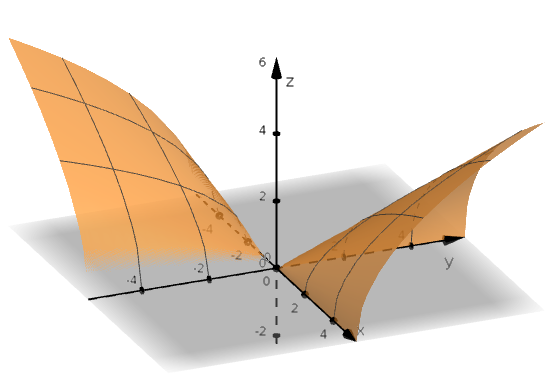
\includegraphics[width=0.5\linewidth]{images/sqrtxy} 

}

\caption{Graph of $f(x,y)=\sqrt{xy}$}\label{fig:unnamed-chunk-1}
\end{figure}

Unfortunately, adding in just one more variable to the function means that we can no longer graph it. If the function were of the form \(w=f(x,y,z)\), the graph would be the set of points \((x,y,z,f(x,y,z))\) which forms a hypersurface in \(\mathbb{R}^4\).

Given a function of two variables (and in the absence of graphing tools) we build up an image of its graph using \emph{level curves} and \emph{cross-sections}.

Level curves intersect the graph of the function with the plane \(z=k\) for values of \(k\) in the range of the function. Plotting a set of level curves gives us a \emph{contour plot} of the function. We generate this plot by setting \(f(x,y)=k\) for a few values of \(k\).

Cross-sections are formed by taking the intersection of \(z=f(x,y)\) with \(x= c\) for a few values of \(c\) and/or by taking the intersection of \(z=f(x,y)\) with \(y= d\) for a few values of \(d\). To make our lives easier, we typically choose \(c=d=0\).

\begin{exercise}
\protect\hypertarget{exr:unlabeled-div-3}{}\label{exr:unlabeled-div-3}

Now it's your turn to have some fun! Choose one of the following functions:

\begin{itemize}
\tightlist
\item
  \(f(x,y) = -3x+y+7\) (mild)
\item
  \(g(x,y)=x^2+4y^2\) (medium)
\item
  \(h(x,y)=3x^2-y^2\) (spicy)
\end{itemize}

\begin{enumerate}
\def\labelenumi{\alph{enumi}.}
\tightlist
\item
  Determine the domain and range of your function.
\item
  Find a few level curves by setting \(f(x,y)=k\), \(g(x,y)=k\), or \(h(x,y)=k\) for at least 4 different values of \(k\). Sketch your level curves below (be sure to label your axes!).
\item
  Sketch the cross-section \(x=0\) below (be sure to label your axes!).
\item
  Sketch the cross-section \(y=0\) below (be sure to label your axes!).
\item
  Based on your level curves and cross-sections, try to sketch the function. You can check all of your answers using the following \href{https://www.geogebra.org/m/zpr5ggau}{interactive applet.}
\end{enumerate}

\end{exercise}

\begin{solution}

Solution for \(f(x,y)=-3x+y+7\)

\begin{enumerate}
\def\labelenumi{\alph{enumi}.}
\item
  The domain is \(\mathbb{R}^2\) and the range is \(\mathbb{R}\)
\item
  Note that we can choose any real value of \(k\) since the range of \(f\) is \(\mathbb{R}\). We have \(-3x+y+7=k\). Rearranging, we find \(y=3x+(k-7)\) which is the equation of a line with slope \(3\) and intercept \(k-7\). Choosing \(k=-1,0,1,2\) we have the family of lines \(y=3x-8\), \(y=3x-7\), \(y=3x-6\), and \(y=3x-5\).
\end{enumerate}

\begin{figure}

{\centering 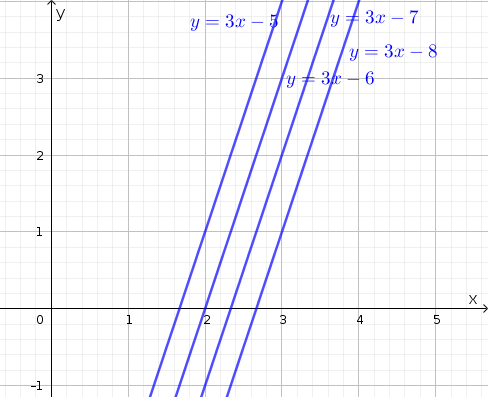
\includegraphics[width=0.5\linewidth]{images/lc-f} 

}

\caption{Level curves of $f(x,y)=-3x+y+7$}\label{fig:unnamed-chunk-2}
\end{figure}

\begin{enumerate}
\def\labelenumi{\alph{enumi}.}
\setcounter{enumi}{2}
\tightlist
\item
  Setting \(x=0\) we have \(f(0,y)=y+7\). Note that this cross-section is in the \(yz\)-plane.
\end{enumerate}

\begin{figure}

{\centering 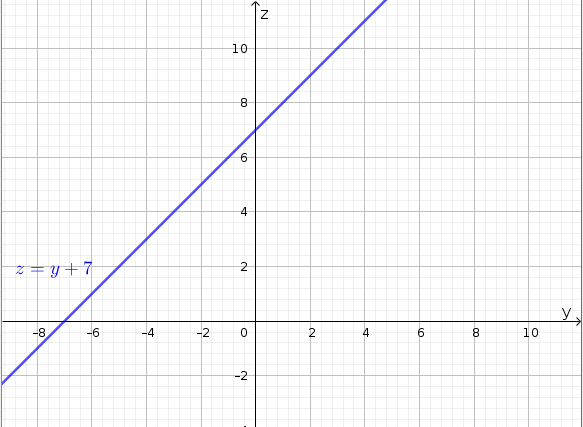
\includegraphics[width=0.5\linewidth]{images/x0-f} 

}

\caption{$x=0$ cross-section of $f(x,y)=-3x+y+7$}\label{fig:unnamed-chunk-3}
\end{figure}

\begin{enumerate}
\def\labelenumi{\alph{enumi}.}
\setcounter{enumi}{3}
\item
  Setting \(y=0\) we have \(f(x,0)=-3x+7\). Note that this cross-section is in the \(xz\)-plane.
\item
  See GeoGebra above.
\end{enumerate}

\end{solution}

\begin{solution}

Solution for \(g(x,y)=x^2+4y^2\)

\begin{enumerate}
\def\labelenumi{\alph{enumi}.}
\item
  The domain is \(\mathbb{R}^2\) and the range is non-negative real numbers (note the sum of squares).
\item
  Note that we must choose \(k\geq 0\) since the range of \(g\) the set of non-negative numbers. We have \(x^2+4y^2=k\), which is the equation of an ellipse. Choosing \(k=0,1,2,3\) we have the family of ellipses \(x^2+4y^2=0\), \(x^2+4y^2=1\), \(x^2+4y^2=2\), and \(x^2+4y^2=3\).
\end{enumerate}

\begin{figure}

{\centering 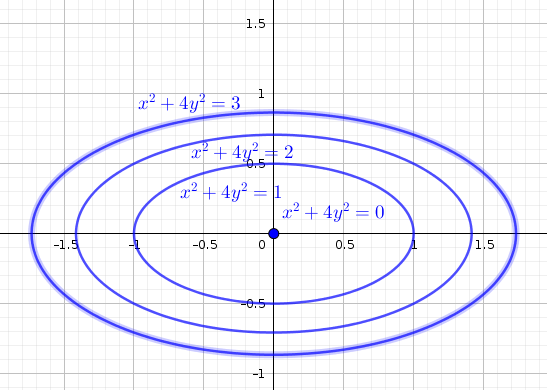
\includegraphics[width=0.5\linewidth]{images/lc-g} 

}

\caption{Level curves of $f(x,y)=x^2+4y^2$}\label{fig:unnamed-chunk-4}
\end{figure}

\begin{enumerate}
\def\labelenumi{\alph{enumi}.}
\setcounter{enumi}{2}
\tightlist
\item
  Setting \(x=0\) we have \(g(0,y)=4y^2\). Note that this cross-section is in the \(yz\)-plane.
\end{enumerate}

\begin{figure}

{\centering 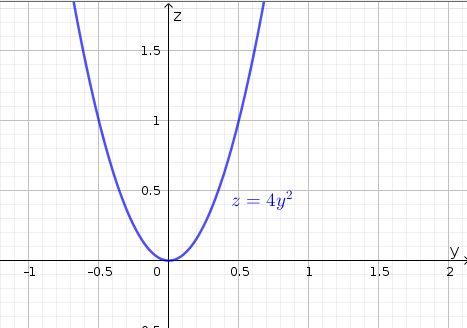
\includegraphics[width=0.5\linewidth]{images/x0-g} 

}

\caption{$x=0$ cross-section of $f(x,y)=x^2+4y^2$}\label{fig:unnamed-chunk-5}
\end{figure}

\begin{enumerate}
\def\labelenumi{\alph{enumi}.}
\setcounter{enumi}{3}
\tightlist
\item
  Setting \(y=0\) we have \(g(x,0)=x^2\). Note that this cross-section is in the \(xz\)-plane.
\end{enumerate}

\begin{figure}

{\centering 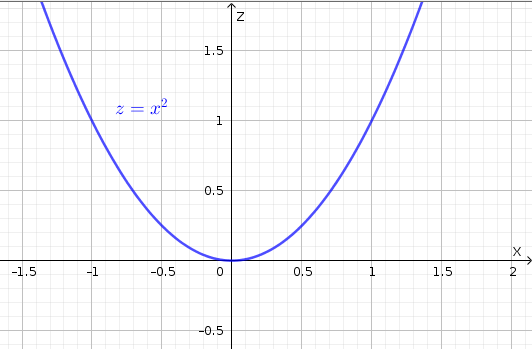
\includegraphics[width=0.5\linewidth]{images/y-0g} 

}

\caption{$y=0$ cross-section of $f(x,y)=x^2+4y^2$}\label{fig:unnamed-chunk-6}
\end{figure}

\begin{enumerate}
\def\labelenumi{\alph{enumi}.}
\setcounter{enumi}{4}
\tightlist
\item
  See GeoGebra above.
\end{enumerate}

\end{solution}

\begin{solution}

Solution for \(h(x,y)=3x^2-y^2\)

\begin{enumerate}
\def\labelenumi{\alph{enumi}.}
\item
  The domain is \(\mathbb{R}^2\) and the range \(\mathbb{R}\).
\item
  Note that we can choose any real value of \(k\) since the range of \(h\) is \(\mathbb{R}\). We have \(3x^2-y^2=k\), which is the equation of a hyperbola. Choosing \(k=-1,0,1,2\) we have the family of hyperbolae \(3x^2-y^2=-1\), \(3x^2-y^2=0\), \(3x^2-y^2=1\), and \(3x^2-y^2=2\).
\end{enumerate}

\begin{figure}

{\centering 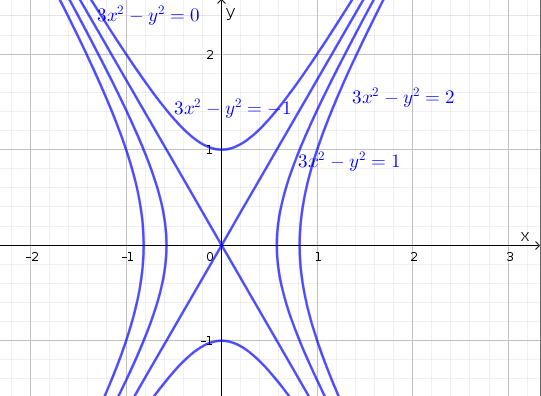
\includegraphics[width=0.5\linewidth]{images/lc-h} 

}

\caption{Level curves of $f(x,y)=3x^2-y^2$}\label{fig:unnamed-chunk-7}
\end{figure}

\begin{enumerate}
\def\labelenumi{\alph{enumi}.}
\setcounter{enumi}{2}
\tightlist
\item
  Setting \(x=0\) we have \(h(0,y)=-y^2\). Note that this cross-section is in the \(yz\)-plane.
\end{enumerate}

\begin{figure}

{\centering 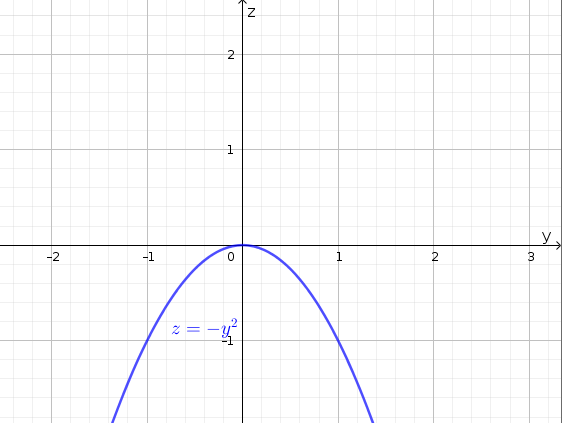
\includegraphics[width=0.5\linewidth]{images/x0-h} 

}

\caption{$x=0$ cross-section of $f(x,y)=3x^2-y^2$}\label{fig:unnamed-chunk-8}
\end{figure}

\begin{enumerate}
\def\labelenumi{\alph{enumi}.}
\setcounter{enumi}{3}
\tightlist
\item
  Setting \(y=0\) we have \(h(x,0)=3x^2\). Note that this cross-section is in the \(xz\)-plane.
\end{enumerate}

\begin{figure}

{\centering 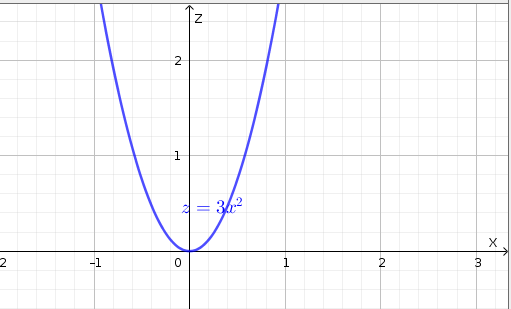
\includegraphics[width=0.5\linewidth]{images/y0-h} 

}

\caption{$y=0$ cross-section of $f(x,y)=3x^2-y^2$}\label{fig:unnamed-chunk-9}
\end{figure}

\begin{enumerate}
\def\labelenumi{\alph{enumi}.}
\setcounter{enumi}{4}
\tightlist
\item
  See GeoGebra above.
\end{enumerate}

\end{solution}

\hypertarget{lec-2}{%
\chapter{Multivariate Limits}\label{lec-2}}

Text References: Course notes pp.~1-10 \& Rogawski 14.1-14.3

\hypertarget{recap}{%
\section{Recap}\label{recap}}

Last time, we learned about scalar fields, which are functions \(f:\mathbb{R}^n\to\mathbb{R}\). We practised calculating the value of such functions given various inputs, and used level curves and cross-sections to graph functions of two variables.

\begin{exercise}
\protect\hypertarget{exr:unlabeled-div-7}{}\label{exr:unlabeled-div-7}

Match the graph of the function to its set of level curves.

\begin{longtable}[]{@{}ll@{}}
\toprule
Level.Curves & Graph.of.Function \\
\midrule
\endhead
1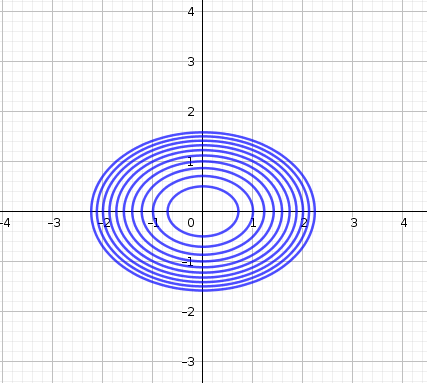
\includegraphics[width=\textwidth,height=1.25in]{images/paraboloid.png} & a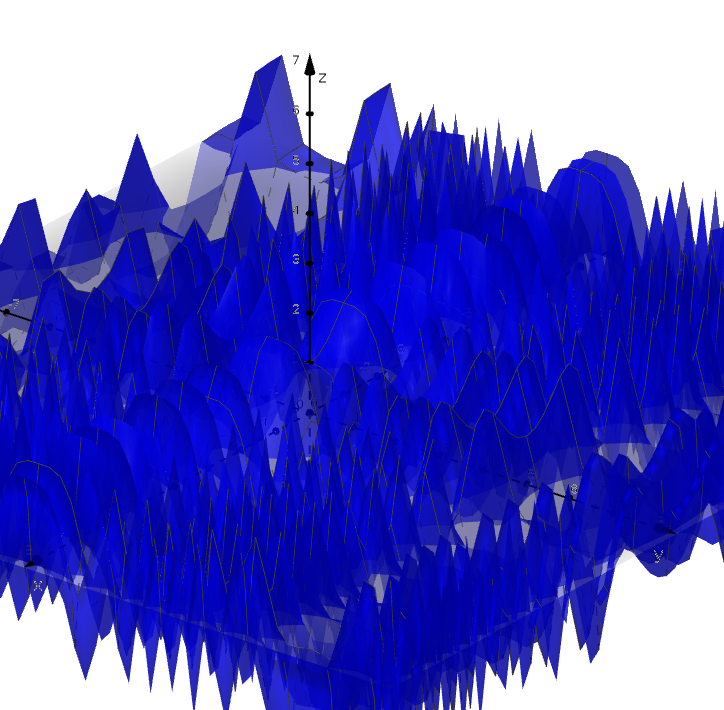
\includegraphics[width=\textwidth,height=1.25in]{images/sin-cos-3d.png} \\
2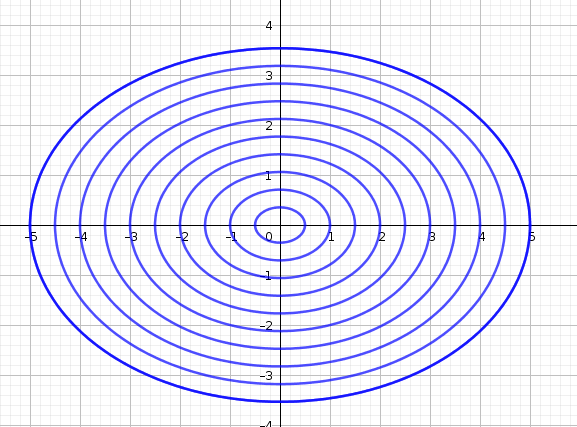
\includegraphics[width=\textwidth,height=1.25in]{images/cone.png} & b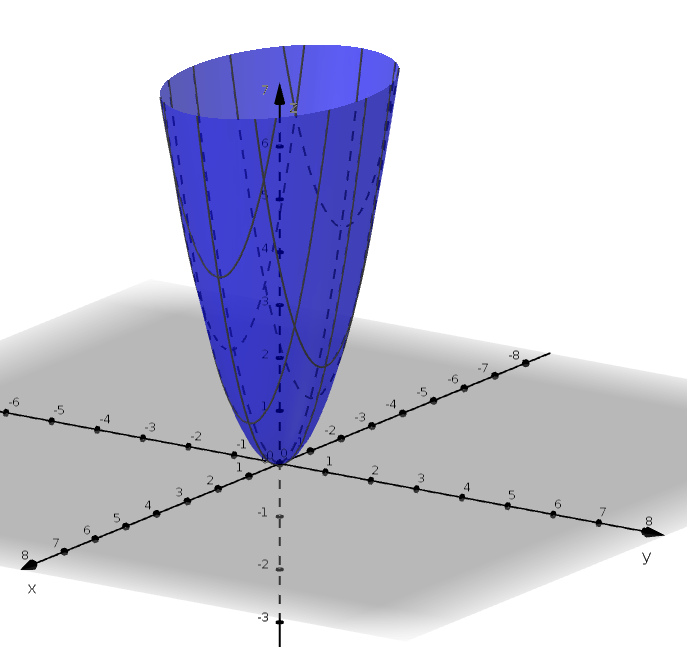
\includegraphics[width=\textwidth,height=1.25in]{images/paraboloid-3d.png} \\
3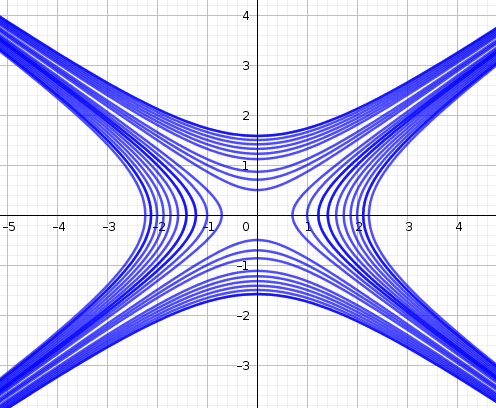
\includegraphics[width=\textwidth,height=1.25in]{images/hyperbola.png} & c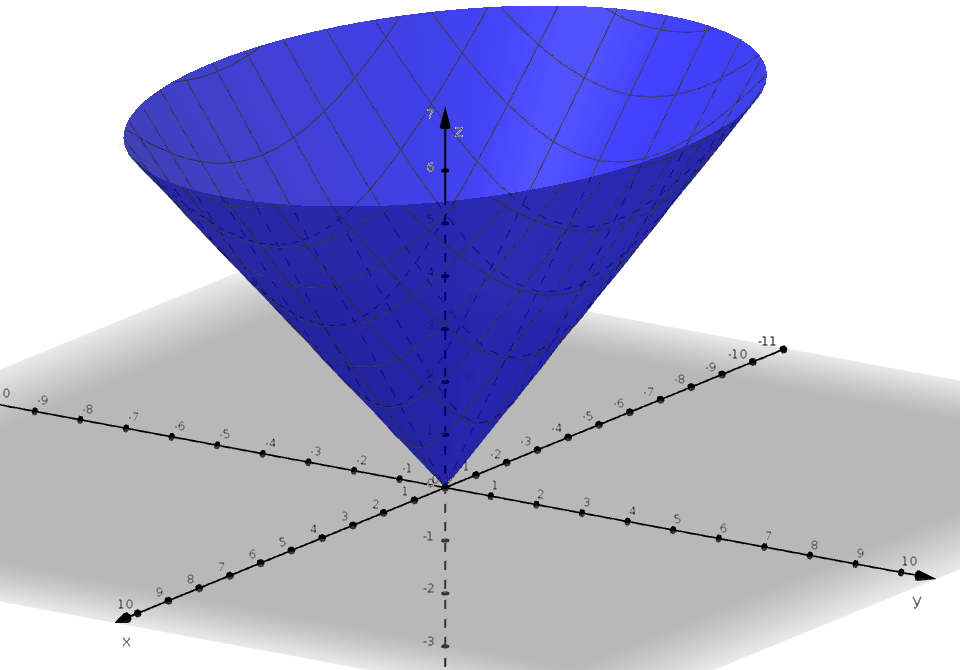
\includegraphics[width=\textwidth,height=1.25in]{images/cone-3d.png} \\
4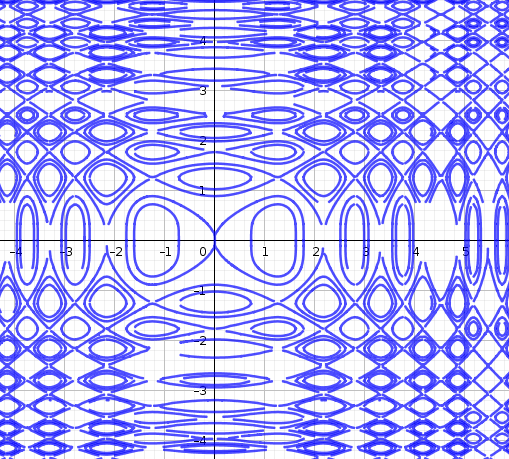
\includegraphics[width=\textwidth,height=1.25in]{images/sin-cos.png} & d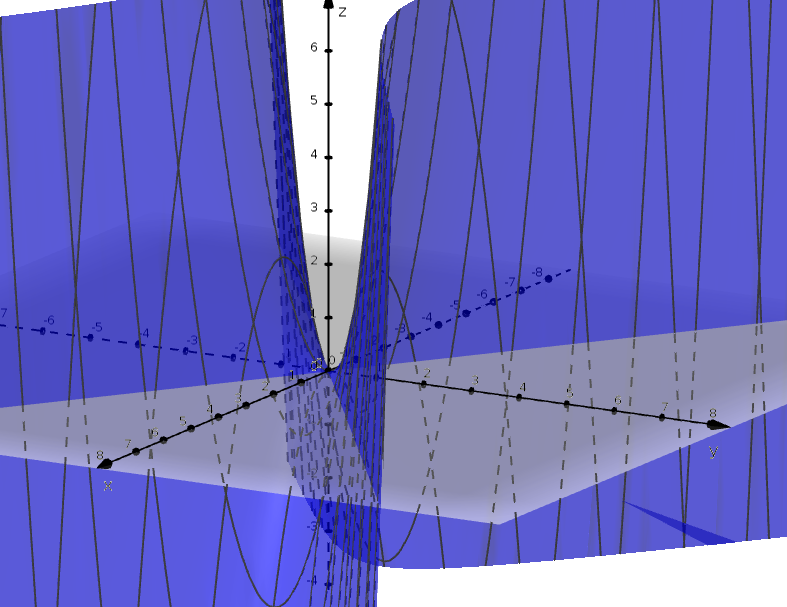
\includegraphics[width=\textwidth,height=1.25in]{images/hyperboloid-3d.png} \\
\bottomrule
\end{longtable}

\end{exercise}

\begin{solution}

1 with b, 2 with c, 3 with d, 4 with a. The trickier set is 1/b and 2/c.~We tell them apart by observing the spacing between the level curves. The closer the level curves are to each other, the steeper the surface. The paraboloid increases in steepness, so we expect its level curves to get closer and closer together. The cone, on the other hand, `opens up' at a constant rate so its level curves are always evenly spaced apart.

\end{solution}

\hypertarget{learning-objectives-1}{%
\section{Learning Objectives}\label{learning-objectives-1}}

\begin{itemize}
\tightlist
\item
  Given a function of 2 variables, consider different paths of approach.
\item
  Outline how to determine whether the limit of a multivariable function exists.
\end{itemize}

\hypertarget{approaching-limit-points}{%
\section{Approaching Limit Points}\label{approaching-limit-points}}

In single-variable calculus, you studied limits of functions. Given a candidate limit point \(a\in\mathbb{R}\), we could approach it either from the left or from the right.

Now, let's consider a function of two variables \(f:\mathbb{R}^2\to\mathbb{R}\) The domain of \(f\) is the \(xy\)-plane. What are ways in which we can approach a candidate limit point \((a,b)\)?

We notice that there are infinitely many ways to approach \((a,b)\)! As you can imagine, this makes determining the limit of a multivariable function much more difficult since we have infinitely many paths to consider.

\begin{example}
\protect\hypertarget{exm:unlabeled-div-9}{}\label{exm:unlabeled-div-9}

Consider \(\displaystyle \lim_{(x,y)\to(0,0)} \dfrac{2xy}{x^2+y^2}\). Approach \((0,0)\) following three distinct paths and for each path calculate the limit.

\begin{itemize}
\tightlist
\item
  Let's approach along the path \(y=0\). Then, \(f(x,0)=\dfrac{2(x)(0)}{x^2+0^2}=0\) for \((x,y)\neq (0,0)\). The limit along this path is \(0\).
\item
  Approaching along the path \(x=0\), we have \(f(0,y)=0\) for \((x,y)\neq (0,0)\). The limit along this path is \(0\).
\item
  Approaching along the path \(y=x\), we have \(f(x,x)=\dfrac{2x^2}{2x^2}=1\) for \((x,y)\neq (0,0)\). The limit along this path is \(1\).
\end{itemize}

\end{example}

\href{https://www.geogebra.org/m/vvywtdnx}{See what's happening in 3D space}

Notice that we found different limits when we approached using different paths. As in single-variable calculus, this is an indication that \(\displaystyle \lim_{(x,y)\to(0,0)} \dfrac{2xy}{x^2+y^2}\) does not exist.

\hypertarget{does-the-limit-exist}{%
\section{Does the Limit Exist?}\label{does-the-limit-exist}}

We won't go through the details of calculating limits for multivariable functions in this course. The short version goes like this:

\begin{itemize}
\tightlist
\item
  If we can find (at least) two paths that yield different limit values, then the limit does not exist.
\item
  To prove that the limit does exist, we need to use the Squeeze Theorem.
\end{itemize}

\begin{exercise}
\protect\hypertarget{exr:unlabeled-div-10}{}\label{exr:unlabeled-div-10}

Consider \(\displaystyle \lim_{(x,y)\to(0,0)} \dfrac{x^3y}{x^6+y^2}\). Find at least two paths of approach that yield different limits. Hint: think about paths that aren't just straight lines.

\href{https://www.geogebra.org/m/rcrgqzqu}{See what's happening in 3D space}

\end{exercise}

\begin{solution}

Let's consider straight lines of the form \(y=mx\) for \(m\in\mathbb{R}\). Note that all of these pass through \((0,0)\) and that the parameter \(m\) allows us to check a family of lines simultaneously.

We have \(f(x,mx) = \dfrac{x^3(mx)}{x^6+(mx)^2} = \dfrac{mx^4}{x^6+m^2x^2}=\dfrac{mx^2}{x^4+m^2}\). As \((x,y)\to(0,0)\), the limit is equal to \(0\).

Now, let's consider the path \(y=x^3\). Notice that this will give us some nice cancellations in the numerator and the denominator: \(f(x,x^3)=\dfrac{x^3(x^3)}{x^6+(x^3)^2}=\dfrac{x^6}{2x^6}\). As \((x,y)\to(0,0)\), the limit is equal to \(\dfrac{1}{2}\).

We've found two paths of approach that yield different limits. Therefore, this limit does not exist.

\end{solution}

\hypertarget{lec-3}{%
\chapter{Partial Derivatives}\label{lec-3}}

Text References: Course notes pp.~1-10 \& Rogawski 14.1-14.3

\hypertarget{recap-1}{%
\section{Recap}\label{recap-1}}

Last time, we discussed how we might show that the limit of a multivariable function does not exist.

\begin{exercise}
\protect\hypertarget{exr:unlabeled-div-12}{}\label{exr:unlabeled-div-12}

Show that \(\displaystyle \lim_{(x,y)\to(0,0)}\dfrac{x^4-y^5}{x^4+y^4}\) does not exist.

\end{exercise}

\begin{solution}

In order to show that the limit does not exist, we need to find (at least) two paths of approach that give different limit values.

Let's try the family of straight lines \(y=mx\):

We have \(\displaystyle \lim_{(x,y)\to(0,0)}\dfrac{x^4-(mx)^5}{x^4+(mx)^4}=\displaystyle \lim_{(x,y)\to(0,0)}\dfrac{x^4(1-m^5x)}{x^4(1+m^4)}=\displaystyle \dfrac{1}{1+m^4}\).

Note that the value of this limit depends on \(m\); this means that approaching along different straight lines will give us different limit values and therefore that the limit does not exist.

\end{solution}

\begin{figure}

{\centering 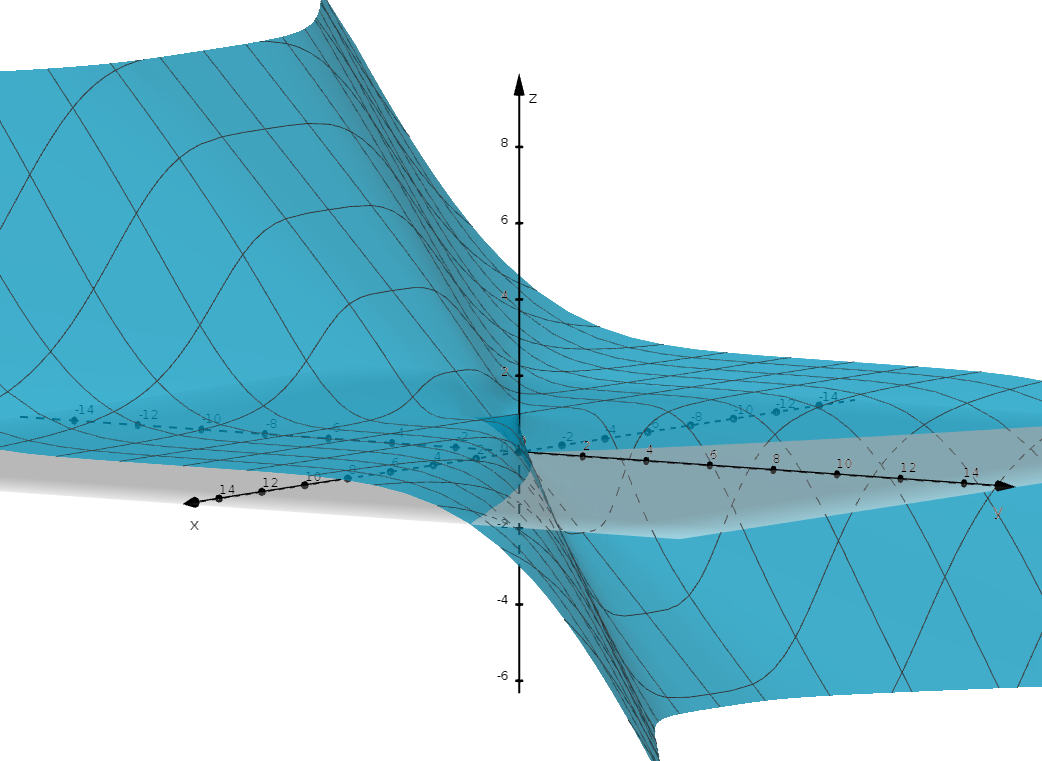
\includegraphics[width=0.5\linewidth]{images/lec-3-ex-1} 

}

\caption{Graph of $f(x,y)=\dfrac{x^4-y^5}{x^4+y^4}$}\label{fig:unnamed-chunk-10}
\end{figure}

See the following \href{https://www.geogebra.org/m/gbyuggth}{3D GeoGebra applet} which shows the graph of the function.

\hypertarget{learning-objectives-2}{%
\section{Learning Objectives}\label{learning-objectives-2}}

\begin{itemize}
\tightlist
\item
  Given a function of several variables, calculate its first-order partial derivatives.
\item
  Given a function of several variables, calculate its higher-order partial derivatives.
\end{itemize}

\hypertarget{first-order-partial-derivative}{%
\section{First Order Partial Derivative}\label{first-order-partial-derivative}}

Now that we're dealing with functions of more than one variable, taking derivatives becomes slightly more complicated. Here are the formal definitions:

\begin{definition}
\protect\hypertarget{def:unlabeled-div-14}{}\label{def:unlabeled-div-14}

The partial derivative of \(f(x,y)\) with respect to \(x\) at the point \((a,b)\) is \[f_x(a,b)=\displaystyle \lim_{h\to 0}\dfrac{f(a+h,b)-f(a,b)}{h}\] and the partial derivative of \(f(x,y)\) with respect to \(y\) at the point \((a,b)\) is \[f_y(a,b)=\displaystyle \lim_{h\to 0}\dfrac{f(a,b+h)-f(a,b)}{h}\] provided that these limits exist.

\end{definition}

\textbf{Notation:} You may see a few different notations: \(f_x\), \(\dfrac{\partial f}{\partial x}\), and \(D_1\) are all used to denote the partial derivative of a multivariable function \(f\) with respect to \(x\) (or, in the case of \(D_1\), whichever variable is listed first).

In practice, we only use these definitions when we run into indeterminate forms. Most of the time, however, we can take partial derivatives by holding one variable constant and differentiating with respect to the other.

\begin{exercise}
\protect\hypertarget{exr:unlabeled-div-15}{}\label{exr:unlabeled-div-15}

Calculate the following partial derivatives:

\begin{enumerate}
\def\labelenumi{\alph{enumi}.}
\tightlist
\item
  \(f_x\) for \(f(x,y)=\sin(xy^2)\)
\item
  \(\dfrac{\partial g}{\partial y}\) for \(g(x,y,z)=xy^2z^3\)
\item
  \(k_x(0,0)\) for \(k(x,y)=(x^3+y^3)^{\frac{1}{3}}\)
\end{enumerate}

\end{exercise}

\begin{solution}

We have

\begin{enumerate}
\def\labelenumi{\alph{enumi}.}
\tightlist
\item
  Holding \(y\) as a constant and differentiating with respect to \(x\), we have \(f_x = y^2cos(xy^2)\).
\item
  Holding \(x\) and \(z\) as constants and differentiating with respect to \(y\), we have \(\dfrac{\partial g}{\partial y}= 2xyz^3\).
\item
  Holding \(y\) as a constant and differentiating with respect to \(x\), we have \[k_x(x,y)=\dfrac{x^2}{(x^3+y^3)^{\frac{2}{3}}}\] If we try to evaluate this at \((x,y)=(0,0)\), we have an indeterminate form. This means that we should use the formal definition to calculate this partial derivative:
\end{enumerate}

\begin{align*}
k_x(0,0)&=\lim_{h\to 0}\dfrac{k(0+h,0)-k(0,0)}{h}\\ &=\lim_{h\to 0}\dfrac{(h^3+0^3)^{\frac{1}{3}}-0}{h}\\&=1
\end{align*}

\end{solution}

\hypertarget{higher-order-partial-derivatives}{%
\section{Higher Order Partial Derivatives}\label{higher-order-partial-derivatives}}

Notice that when we take first-order partial derivatives, we still end up with multivariable functions. We can keep taking partial derivatives for as long as we like! For now, we'll stick to second-order partial derivatives.

Given a function \(f(x,y)\), we found that it had two partial derivatives: \(f_x\) and \(f_y\). If we take partial derivatives of the partial derivatives, we will end up with four second-order partial derivatives: \(f_{xx}\), \(f_{xy}\), \(f_{yx}\), and \(f_{yy}\).

\textbf{Notation:} We have to be a little careful with notation here.

\begin{itemize}
\tightlist
\item
  Notation of the form \(f_{xy}\) is read from \emph{left to right}: it means that first, we take the partial derivative w.r.t \(x\) and second, we take the partial derivative w.r.t \(y\).
\item
  Notation of the form \(\dfrac{\partial^2 f}{\partial x\partial y}\) is read from \emph{right to left}: it means that first, we take the partial derivative w.r.t \(y\) and second, we take the partial derivative w.r.t \(x\).
\item
  Notation of the form \(D_1D_2f\) is read from from \emph{right to left}: it means that first, we take the partial derivative w.r.t \(y\) and second, we take the partial derivative w.r.t \(x\).
\end{itemize}

\begin{exercise}
\protect\hypertarget{exr:unlabeled-div-17}{}\label{exr:unlabeled-div-17}

Calculate all of the second partial derivatives of \(f(x,y)=xe^{2xy}\). What do you notice?

\end{exercise}

\begin{solution}

We have \[ f_x(x,y)=e^{2xy}+2xye^{2xy} \quad \mbox{and} \quad f_y(x,y)=2x^2e^{2xy}\]
And therefore
\begin{align*}
        f_{xx}(x,y)&=4ye^{2xy}+4xy^2e^{2xy}\\
        f_{xy}(x,y)&=4xe^{2xy}+4x^2ye^{2xy}\\
        f_{yx}(x,y)&=4xe^{2xy}+4x^2ye^{2xy}\\
        f_{yy}(x,y)&=4x^3e^{2xy}\\
    \end{align*}

We notice that the mixed partial derivatives, \(f_{xy}\) and \(f_{yx}\) are equal.

\end{solution}

A natural question that arises is whether this phenomenon always occurs. Clairaut's Theorem provides an answer:

\begin{theorem}[Clairaut's Theorem]
\protect\hypertarget{thm:unlabeled-div-19}{}\label{thm:unlabeled-div-19}

If \(f_{xy}\) and \(f_{yx}\) are defined in some neighbourhood of \((a,b)\) and are both continuous at \((a,b)\), then \(f_{xy}(a,b)=f_{yx}(a,b)\).

\end{theorem}

In this course, the functions that we'll work with will generally be nice, so this theorem applies. Clairaut's Theorem also generalizes to higher-order partial derivatives, which is quite handy. One way to use this theorem is to simplify calculations involving mixed partial derivatives.

\begin{exercise}
\protect\hypertarget{exr:unlabeled-div-20}{}\label{exr:unlabeled-div-20}

Let \(f(x,y,z,w)=x^3w^2z^2+\sin\left(\dfrac{xy}{z^2} \right)\). Calculate \(f_{zzwx}\).

\end{exercise}

\begin{solution}

Note that the second term does not depend on \(w\); differentiating first w.r.t \(w\) will make this term disappear. Applying Clairaut's Theorem, we have \(f_{zzwx}=f_{wzzx}\).

Taking the partial derivative w.r.t \(w\), we have \[f_w = 2x^3wz^2\]

Then, taking the partial derivative w.r.t \(z\), we have \[f_{wz}=4x^3wz\]

Taking the partial derivative w.r.t \(z\) a second time, we have \[f_{wzz}=4x^3w\]

Finally, taking the partial derivative w.r.t \(x\), we have \[f_{wzzx} =12x^2w \]

\end{solution}

\hypertarget{lec-4}{%
\chapter{Tangent Planes, Linear Approximation and Differentials}\label{lec-4}}

Text References: Course notes pp.~10-22 \& Rogawski 14.4, 11.1, 14.6

\hypertarget{recap-2}{%
\section{Recap}\label{recap-2}}

Last time, we learned how to calculate first and higher-order partial derivatives of functions. As we'll learn, partial derivatives are key to helping us calculate tangent planes and linear approximations.

\begin{exercise}
\protect\hypertarget{exr:unlabeled-div-22}{}\label{exr:unlabeled-div-22}

At which point above the \(xy\)-plane will both partial derivatives be positive?

\begin{enumerate}
\def\labelenumi{\alph{enumi}.}
\tightlist
\item
  \((-5, -5)\)
\item
  \((5, -5)\)
\item
  \((5, 5)\)
\item
  \((-5, 5)\)
\end{enumerate}

\begin{center}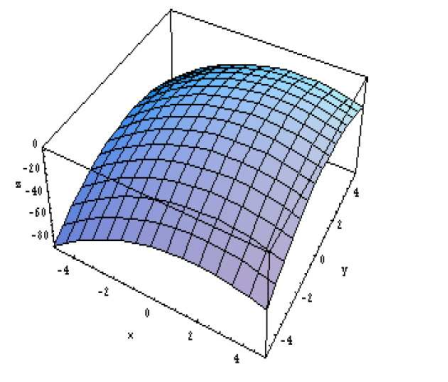
\includegraphics[width=0.5\linewidth]{images/l4-recap} \end{center}

\end{exercise}

\begin{solution}

The answer is a. At this point, both tangent lines (along the \(x\) and \(y\) directions) have a positive slope. In other words, the surface is moving upward in both the \(x\) and \(y\) directions at this point.

\end{solution}

\hypertarget{learning-objectives-3}{%
\section{Learning Objectives}\label{learning-objectives-3}}

\begin{itemize}
\tightlist
\item
  Given a surface and a point, find the tangent plane to the surface at the point.
\item
  Given a multivariable function, find its linear approximation and use it to approximate the value of the function at a given point.
\item
  Use the differential to calculate change with respect to a given variable.
\end{itemize}

\hypertarget{tangent-planes}{%
\section{Tangent Planes}\label{tangent-planes}}

In single-variable calculus, we learned about the linear approximation to a function. Given a curve \(y=f(x)\) at a point \((x_0, f(x_0))\), the linear approximation of \(f\) at \(x_0\) is given by \(L_{x_0}=f(x_0)+f'(x_0)(x-x_0)\). Our next task is to generalize this to multivariate functions. Our first observation is that for surfaces of the form \(z=f(x,y)\), we will get a \textbf{tangent plane} rather than a tangent line.

Let's think for a moment about the partial derivatives of a function. Given a point \((x_0,y_0)\), \(f_x(x_0,y_0)\) gives the slope of the tangent line to the cross-section \(y=y_0\) (remember, we're holding \(y\) as a constant to calculate the partial derivative w.r.t \(x\)) and \(f_y(x_0, y_0)\) gives the slope of the cross-section \(x=x_0\).

From a derivation in your course notes, a non-vertical plane passing through the point \((x_0, y_0, z_0)\) will have equation \[z=z_0+A(x-x_0)+B(y-y_0)\] where \(A\) and \(B\) are constants.

Setting \(y=y_0\), we have \(z=z_0+A(x-x_0)\). Note that we are on the cross-section \(y=y_0\), which we know to have slope equal to \(f_x(x_0, y_0)\). This means that \(A=f_x(x_0,y_0)\). We make a similar argument to find that \(B=f_y(x_0,y_0)\) and therefore the equation of the tangent plane is \[z=z_0+f_x(x_0, y_0)(x-x_0)+f_y(x_0, y_0)(y-y_0)\]

\begin{exercise}
\protect\hypertarget{exr:unlabeled-div-24}{}\label{exr:unlabeled-div-24}

Find the equation of the tangent plane to the surface \(z=\sqrt{x^2+y^2}\) at the point \((3, -4)\).

\end{exercise}

\begin{solution}

We have \(x_0=3, y_0=-4\), and \(z_0=f(x_0,y_0)=\sqrt{3^2+(-4)^2}=5\).

Furthermore, \(f_x = \dfrac{x}{\sqrt{x^2+y^2}}\) and\(f_y = \dfrac{y}{\sqrt{x^2+y^2}}\). Evaluating at the point \((3, 4)\), we have \(f_x(3,4)=\frac{3}{5}\) and \(f_y(3, -4)=-\frac{4}{5}\).

Putting everything together, we find that the tangent plane at point \((3,-4)\) has equation \[z=5+\frac{3}{5}(x-3)-\frac{4}{5}(y+4)\]

\end{solution}

\hypertarget{linear-approximation}{%
\section{Linear Approximation}\label{linear-approximation}}

We often use the equation of the tangent plane to approximate values of a given function. As long as we're close enough to the point \((x_0, y_0)\), we can approximate the value of \(f(x,y)\) at a nearby point: \[f(x,y)\approx f(x_0,y_0)+f_x(x_0, y_0)(x-x_0)+f_y(x_0, y_0)(y-y_0)\]

\begin{exercise}
\protect\hypertarget{exr:unlabeled-div-26}{}\label{exr:unlabeled-div-26}

Approximate the value of \(f(x,y)=\sqrt{x^2+y^2}\) at the point \((3.01, -3.99)\)

\end{exercise}

\begin{solution}

Using the linear approximation we found earlier, we have
\begin{align*}
f(x,y) & \approx 5+\frac{3}{5}(x-3)-\frac{4}{5}(y+4) \\
& \approx 5+\frac{3}{5}(3.01-3)-\frac{4}{5}(-3.99+4)\\
& \approx 4.998
\end{align*}

Note that this is quite close to the actual value of \(4.99802\)!

\end{solution}

\hypertarget{differentials}{%
\section{Differentials}\label{differentials}}

When working with linear approximations, it's common to use differential notation by setting \(\Delta x = x-x_0\), \(\Delta y = y- y_0\), and \(\Delta f = f(x,y)-f(x_0, y_0)\). In this case, we can rewrite the linear approximation as \[\Delta f = f_x(x_0, y_0)\Delta x + f_y(x_0, y_0) \Delta y\]

Notice that the closer we get to the point \((x_0, y_0)\), that is, as \(\Delta x \to 0\) and \(\Delta y \to 0\), the more accurate our approximation. It's therefore common to replace the \(\Delta\) symbols with \(d\)-notation and the \(\approx\) with an equal sign to get an even more compact expression \[df = f_x dx+f_y dy\] Keep in mind, however, that the point \((x_0, y_0)\) is still playing a role here.

Let's see how the notation of differentials can be useful.

\begin{exercise}
\protect\hypertarget{exr:unlabeled-div-28}{}\label{exr:unlabeled-div-28}

An isosceles triangle has base \(4\)m and equal angles of \(\frac{\pi}{4}\). How sensitive is the triangle's area to small variations in the length of the base and the equal angles?

\end{exercise}

\begin{solution}

Note that the height of an isosceles triangle like the one described in this exercise is given by \(\frac{b}{2}\tan(\theta)\). Therefore, the area of the triangle is given by \(A(b, \theta)= \frac{b^2 \tan(\theta)}{4}\).

The differential at \((4, \pi/4)\) is \(dA= \dfrac{\partial A}{\partial b}db + \dfrac{\partial A}{\partial \theta}d\theta\). Calculating the partial derivatives, we find that the change in areas is approximately
\begin{align*}
dA &= \frac{\tan(\pi/4)}{2}db + 4 \sec^2(\pi/4)d\theta\\  
&= db + 8 d\theta
\end{align*}

Therefore the area of the triangle is \(8\) times more sensitive to changes in the equal angles compared to changes in the length of its base.

\end{solution}

\hypertarget{lec-5}{%
\chapter{Parametric Curves}\label{lec-5}}

Text References: Course notes pp.~10-22 \& Rogawski 14.4, 11.1, 14.6

\hypertarget{recap-3}{%
\section{Recap}\label{recap-3}}

Last time, we discussed the equation of tangent planes and how to use them to approximate values of a function at a given point.

\begin{exercise}
\protect\hypertarget{exr:unlabeled-div-30}{}\label{exr:unlabeled-div-30}

You measure a cylinder that has a height of \(3.34\) meters and a radius of \(2.77\) meters. If the measurement error of the height is \(2\)cm and the measurement error of the radius is \(3\)cm, what is the measurement error on the volume of the cylinder?

\end{exercise}

\begin{solution}

We know that the volume of the cylinder is given by \(V(r, h)=\pi r^2 h\). Using the differential form of the linear approximation, we have
\begin{align*}
dV &= V_r dr+ V_h dh \\
&= 2\pi r h dr + \pi r^2 dh\\
&= 2\pi(2.77)(3.34)(0.03)+\pi(2.77)^2(0.02)\\
&=2.23 m^3
\end{align*}

\end{solution}

\hypertarget{learning-objectives-4}{%
\section{Learning Objectives}\label{learning-objectives-4}}

\begin{itemize}
\tightlist
\item
  Calculate the speed, velocity, and acceleration of a particle whose movement is described by a vector function.
\item
  Use vector functions to describe curves and paths in parametric form.
\end{itemize}

\hypertarget{vector-functions}{%
\section{Vector Functions}\label{vector-functions}}

In single-variable calculus, we learned how to parametrize curves by describing a point \((x,y)\) using the variable \(t\) and thinking of \(x\) and \(y\) as functions of \(t\). This parametric description allows us to describe a broader set of relations between \(x\) and \(y\). Not only that, but we now get additional information about the direction of the curve and its speed. It's common to distinguish between the \textbf{curve} and its \textbf{path}. the curve is what gets `traced' on paper; the path describes how that `tracing' is done. As you might imagine, there are infinitely many ways to parametrize a given curve!

The \href{https://www.geogebra.org/m/kffabg55}{interactive applet} illustrates this difference. Use the checkboxes to select one of the two parametric curves and advance the slider for \(t\in [0, 2\pi]\) to view the path along which the curve is drawn. Notice how both curves are the same, but their paths are different.

Given that we're thinking of both \(x\) and \(y\) as functions of \(t\), we can think of the corresponding parametric equations as \textbf{vector functions} which take a scalar as input and output a vector, that is, \(\vec{r}: \mathbb{R}\to\mathbb{R}^n\). The vector \(\vec{r}(t)\) is interpreted as starting from the origin so that its tip traces out the path described by the parametric curves.

Given a vector function \(\vec{r}(t)=\begin{bmatrix}x(t)\\y(t)\end{bmatrix}\), we define its derivative as \(\vec{r}'(t)=\begin{bmatrix}x'(t)\\y'(t)\end{bmatrix}\). If we interpret \(\vec{r}(t)\) as describing the motion of a point, \(\vec{r}'(t)\) gives its velocity, \(\Vert \vec{r}'(t)\Vert\) gives its speed, and \(\vec{r}''(t)\) gives the acceleration.

\begin{exercise}
\protect\hypertarget{exr:unlabeled-div-32}{}\label{exr:unlabeled-div-32}

Consider a particle moving according to the vector function \(\vec{r}(t)=\begin{bmatrix}\cos(2t)\sin(t)\\ \sin(3t)\end{bmatrix}\). Determine

\begin{enumerate}
\def\labelenumi{\alph{enumi}.}
\tightlist
\item
  the velocity;
\item
  the speed; and
\item
  the acceleration
\end{enumerate}

of the particle.

\end{exercise}

\begin{solution}

We have \(\vec{r}(t)=\begin{bmatrix}x(t)\\y(t)\end{bmatrix}\) where \(x(t)=\cos(2t)t\) and \(y(t)=\sin(3t)\). Taking the derivative of each component, we find the velocity: \[\vec{v}(t)=\vec{r}'(t)=\begin{bmatrix}\cos(2t)-2t\sin(2t)\\ 3\cos(3t) \end{bmatrix}\] The speed is therefore \[\Vert\vec{v}(t)\Vert= \sqrt{(\cos(2t)-2t\sin(2t))^2+(3\cos(3t))^2} = \sqrt{9 \cos^2(3 t) + (\cos(2 t) - 2 t \sin(2 t))^2}\]

Finally, taking derivatives once more, we find the acceleration: \[\vec{a}(t)=\vec{r}''(t)=\begin{bmatrix}-4 (\sin(2 t) + t \cos(2 t)) \\ -27\cos(3t)\end{bmatrix}\]

\end{solution}

\hypertarget{parametrization-of-curves}{%
\section{Parametrization of Curves}\label{parametrization-of-curves}}

\hypertarget{circles}{%
\subsection{Circles}\label{circles}}

So far, we've seen how to parametrize circles; a standard for parametrizing a circle of radius \(a\) is \[\vec{r}(t)=\begin{bmatrix}a\cos(\omega t)\\ a\sin(\omega t)\end{bmatrix} \quad \mbox{where $\omega$ is the angular frequency}\]

The \href{https://www.geogebra.org/m/d7wfdtgt}{interactive applet} illustrates this standard parametrization of a circle. Start by tracing the curve by moving the slider for \(t\) when \(a=1\) and \(\omega=1\). See how the curve and path change as the values of \(a\) and \(\omega\) change.

Let's take a look at a few other types of curves.

\hypertarget{ellipses}{%
\subsection{Ellipses}\label{ellipses}}

Related to circles are ellipses; in fact, circles can be thought of as a sub-case of ellipses.

\begin{exercise}
\protect\hypertarget{exr:unlabeled-div-34}{}\label{exr:unlabeled-div-34}

Give parametric equations for the ellipse with equation \(9x^2+y^2=4\)?

\end{exercise}

\begin{solution}

Note that \(-\frac{2}{3}\leq x\leq \frac{2}{3}\) and \(-2\leq y \leq 2\). We can find these bounds by setting \(y=0\) and \(x=0\), respectively.

Working from the parametrization of a circle and taking the above constraints into account, we find \[\vec{r}(t)=\begin{bmatrix}\frac{2}{3}\cos(\omega t) \\ 2\sin(\omega t)\end{bmatrix}, \quad t\in [0, 2\pi/\omega]\]

\end{solution}

What if we want to shift the centre of the ellipse to a point other than \((0,0)\)?

\begin{exercise}
\protect\hypertarget{exr:unlabeled-div-36}{}\label{exr:unlabeled-div-36}

Give parametric equations for the ellipse with equation \(9(x+1)^2+(y-3)^2=4\)?

\end{exercise}

\begin{solution}

Note that this is the same ellipse as the previous exercise, but centred at \((-1, 3)\). We need to apply these shifts to the parametric equations:

\[\vec{r}(t)=\begin{bmatrix}\frac{2}{3}\cos(\omega t) -1 \\ 2\sin(\omega t)\end{bmatrix}+3, \quad t\in [0, 2\pi/\omega]\]

\end{solution}

In the \href{https://www.geogebra.org/m/mehspkdt}{interactive applet}, you can enter your own parametrizations and observe the behaviour of the curve. Try inputting the parametrizations from the previous two examples to verify your work.

\hypertarget{lines}{%
\subsection{Lines}\label{lines}}

A common curve to parametrize is a straight line passing that starts from the point \((x_0,y_0)\) and ends at the point \(x_1, y_1\). We can parametrize as follows: \[\vec{r}(t)=\begin{bmatrix}x_0+(x_1-x_0)t \\ y_0 + (y_1-y_0)t\end{bmatrix}, t\in[0,1]\]

\begin{exercise}
\protect\hypertarget{exr:unlabeled-div-38}{}\label{exr:unlabeled-div-38}

Give parametric equations for the straight line segment from \((-1,3)\) to \((2, 9\).

\end{exercise}

\begin{solution}

We have \((x_0, y_0)=(-1,3)\) and \((x_1, y_1)=(2,9)\). Therefore a parametrization is given by \[\vec{r}(t)=\begin{bmatrix}-1+3t \\  3+ 6t\end{bmatrix}, \quad t\in[0,1]\]

\end{solution}

\hypertarget{curves-of-the-form-yfx}{%
\subsection{\texorpdfstring{Curves of the form \(y=f(x)\)}{Curves of the form y=f(x)}}\label{curves-of-the-form-yfx}}

Finally, we can also parametrize curves of the form \(y=f(x)\); in fact, the parametrization has already been done for us in this case with \(x\) as the parameter. Using \(t\) instead, we get \[\vec{r}(t)=\begin{bmatrix}t \\f(t)\end{bmatrix}\]

\hypertarget{lec-6}{%
\chapter{Chain rule for paths}\label{lec-6}}

Text References: Course notes pp.~26-37 \& Rogawski 14.5-14.7

\hypertarget{recap-4}{%
\section{Recap}\label{recap-4}}

Last time, we learned how to parametrize several different types of curves and to represent these parametrizations using vector functions.

\begin{exercise}
\protect\hypertarget{exr:unlabeled-div-40}{}\label{exr:unlabeled-div-40}

What does the path of the particle described by \(x(t)=\cos(t), y(t)=\sin(t), z(t)=-t\) for \(0\leq t \leq 10\) look like?

\begin{enumerate}
\def\labelenumi{\alph{enumi}.}
\tightlist
\item
  a circle in the \(xz\)-plane
\item
  a helix on which the particle is travelling up
\item
  a helix on which the particle is travelling down
\item
  a sine wave in the \(xz\)-plane
\end{enumerate}

\end{exercise}

\begin{solution}

Recall that on the \(xy\)-plane, \(x(t)=\cos(t), y(t)=\sin(t)\) parametrizes a circle. Thus, viewed from above, the particle is travelling on the unit circle. This means that the particle is following a helical path. As the value of \(t\) increases, the value of \(z\) decreases and therefore the particle is travelling downward.

\href{https://www.geogebra.org/m/n7axse42}{See what's happening in 3D space}

\end{solution}

\hypertarget{learning-objectives-5}{%
\section{Learning Objectives}\label{learning-objectives-5}}

\begin{itemize}
\tightlist
\item
  Apply the Chain Rule to calculate derivatives of multivariate functions with arbitrarily many intermediate and independent variables
\end{itemize}

\hypertarget{chain-rule-for-paths}{%
\section{Chain Rule for Paths}\label{chain-rule-for-paths}}

Consider a function \(f(x,y)\) where \(x\) and \(y\) are themselves functions of a parameter \(t\). Setting \(z=f(x,y)\), we can represent the relationship between the variables with a dependence tree:

\begin{figure}

{\centering 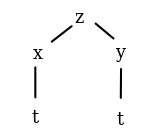
\includegraphics[width=0.2\linewidth]{images/basic-dt} 

}

\caption{Dependence tree of $z=f(x,y)$ where $x$ and $y$ are both functions of $t$}\label{fig:unnamed-chunk-12}
\end{figure}

This dependence tree is useful in Chain Rule calculations. Given \(z=f(x,y)\) where \(x\) and \(y\) are themselves functions of a parameter \(t\), we realize that \(z\) does, in fact, depend on the parameter \(t\) (via \(x(t)\) and \(y(t)\). One question we can ask ourselves is how to determine the derivative of \(z\) with respect to \(t\). From our differentials, we get \[dz=\dfrac{\partial z}{\partial x}dx + \dfrac{\partial z}{\partial y}dy\]
dividing by the infinitesimal \(dt\), we get the \textbf{Chain Rule for Paths}: \[\dfrac{dz}{dt}=\dfrac{\partial z}{\partial x}\dfrac{dx}{dt}+\dfrac{\partial z}{\partial y}\dfrac{dy}{dt}\]

Notice how there is one summand for each path in the dependence tree, and that each summand is gotten by multiplying the appropriate derivatives, which we can find by looking at the branches!

\begin{exercise}
\protect\hypertarget{exr:unlabeled-div-42}{}\label{exr:unlabeled-div-42}

Let \(z=f(x,y)=1+x^2+y^2\) with \(x(t)=e^t\sin(t)\) and \(y(t)=2e^t\cos(t)\). Find the value of \(\dfrac{dz}{dt}\) at \(t=0\).

\end{exercise}

\begin{solution}

By the Chain Rule for paths, we know that \(\dfrac{dz}{dt}=\dfrac{\partial z}{\partial x}\dfrac{dx}{dt}+\dfrac{\partial z}{\partial y}\dfrac{dy}{dt}\). Let's break things into smaller pieces.

\begin{itemize}
\tightlist
\item
  \(\dfrac{\partial z}{\partial x}=2x\)
\item
  \(\dfrac{\partial z}{\partial y}=2y\)
\item
  \(\dfrac{dx}{dt}=e^t\sin(t)+e^t\cos(t)\)
\item
  \(\dfrac{dy}{dt}=2e^t\cos(t)-2e^t\sin(t)\)
\end{itemize}

Putting things together, we get \[\dfrac{dz}{dt}= 2x (e^t\sin(t)+e^t\cos(t)) + 2y(2e^t\cos(t)-2e^t\sin(t))\]

Now, we can use the fact that \(t=0\), substitute it in the above equation, and use it to find \(x(0)=0\) and \(y(0)=2\) to get \[\left .\dfrac{dz}{dt}\right|_{t=0} = 2(0)(0+1)+2(2)(2-0)=8\]

\end{solution}

\hypertarget{generalized-chain-rule}{%
\section{Generalized Chain Rule}\label{generalized-chain-rule}}

Now, let's consider \(z=f(x,y)\) where \(x\) and \(y\) are themselves multivariate functions. Let's suppose that \(x=g_1(s,t)\) and \(y=g_2(s,t)\). We have the following dependence tree:\\

\begin{figure}

{\centering 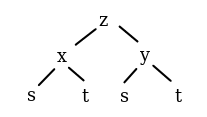
\includegraphics[width=0.3\linewidth]{images/gen-dt} 

}

\caption{Dependence tree of $z=f(x,y)$ where $x=g_1(s,t)$ and $y=g_2(s,t)$}\label{fig:unnamed-chunk-13}
\end{figure}

Now, \(z\) depends on both \(s\) and \(t\). Using the tree as a guide, we can calculate the partial derivatives of \(z\) with respect to these two variables:
\begin{align*}
\dfrac{\partial z}{\partial s}& = \dfrac{\partial z}{\partial x}\dfrac{\partial x}{\partial s} +\dfrac{\partial z}{\partial y}\dfrac{\partial y}{\partial s}  \\
\dfrac{\partial z}{\partial t} &=\dfrac{\partial z}{\partial x}\dfrac{\partial x}{\partial t} +\dfrac{\partial z}{\partial y}\dfrac{\partial y}{\partial t}
\end{align*}

Let's pay attention to notation for a moment:

\begin{itemize}
\tightlist
\item
  We use \(\partial\) to denote a partial derivative; that is, when the function being differentiated depends on more than one variable
\item
  We use \(d\) to denote a derivative; that is, when the function being differentiated depends on a single variable.
\end{itemize}

\begin{exercise}
\protect\hypertarget{exr:unlabeled-div-44}{}\label{exr:unlabeled-div-44}

Let \(z=f(x,y)\) where \(x=g(r,s)\), \(y= h(r)\), and \(r=p(t)\). Draw the dependence diagram and give the Chain Rule for \(\dfrac{\partial z}{\partial s}\) and \(\dfrac{\partial z}{\partial t}\)

\end{exercise}

\begin{solution}

The dependence tree is as follows:

\begin{figure}

{\centering 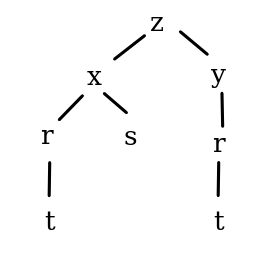
\includegraphics[width=0.2\linewidth]{images/ex-dt} 

}

\caption{Dependence tree of $z=f(x,y)$ where $x=g(s,t)$, $y=h(r)$, and $r=p(t)$}\label{fig:unnamed-chunk-14}
\end{figure}

To calculate the partial derivative of \(z\) with respect to \(s\), we must follow and sum the paths that start from \(z\) and end at \(s\). We get \[\dfrac{\partial z}{\partial s} = \dfrac{\partial z}{\partial x}\dfrac{\partial x}{\partial s}\]

To calculate the partial derivative of \(z\) with respect to \(t\), we must follow and sum the paths that start from \(z\) and end at \(t\). We get \[\dfrac{\partial z}{\partial t} = \dfrac{\partial z}{\partial x}\dfrac{\partial x}{\partial r}\dfrac{dr}{dt}+\dfrac{\partial z}{\partial y}\dfrac{\partial y}{\partial r}\dfrac{dr}{dt}\]

\end{solution}

\hypertarget{lec-7}{%
\chapter{Gradients and Directional Derivatives}\label{lec-7}}

Text References: Course notes pp.~26-37 \& Rogawski 14.5-14.7

\hypertarget{recap-5}{%
\section{Recap}\label{recap-5}}

Last time, we learned how to use dependence trees to compute Chain Rules.

\begin{exercise}
\protect\hypertarget{exr:unlabeled-div-46}{}\label{exr:unlabeled-div-46}

Let \(z=f(x,y)\) where \(x=r\cos(\theta)\) and \(y=r\sin(\theta)\). If \(z=x^2y\), use the Chain Rule to calculate \(\left. \dfrac{\partial z}{\partial r} \right|_{r=1,\theta=0}\)

\end{exercise}

\begin{solution}

The dependence tree is as follows:

\begin{figure}

{\centering 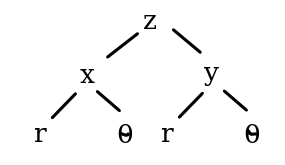
\includegraphics[width=0.2\linewidth]{images/recap-de} 

}

\caption{Dependence tree of $z=f(x,y)$ where $x=g(r,\theta)$, and $y=h(r,\theta)$}\label{fig:unnamed-chunk-15}
\end{figure}

To calculate the partial derivative of \(z\) with respect to \(r\), we must follow and sum the paths that start from \(z\) and end at \(r\). We get \[\dfrac{\partial z}{\partial r} = \dfrac{\partial z}{\partial x}\dfrac{\partial x}{\partial r}+ \dfrac{\partial z}{\partial y}\dfrac{\partial y}{\partial r}\]

We have

\begin{itemize}
\tightlist
\item
  \(\dfrac{\partial z}{\partial x} = 2x\)
\item
  \(\dfrac{\partial z}{\partial y} = x^2\)
\item
  \(\dfrac{\partial x}{\partial r} = \cos(\theta)\)
\item
  \(\dfrac{\partial y}{\partial r} = \sin(\theta)\)
\end{itemize}

At \((r,\theta)=(1,0)\), we have \(x(1,0)=1\) and \(y=(1,0)=0\). Substituting everything into the Chain Rule, we get \[\left .\dfrac{\partial z}{\partial r}\right|_{r=1, \theta=0} =2(1)(1)+ 1^2(0)=2\]

\end{solution}

\hypertarget{learning-objectives-6}{%
\section{Learning Objectives}\label{learning-objectives-6}}

\begin{itemize}
\tightlist
\item
  Given a function of several variables, calculate its gradient vector and evaluate it at a point.
\item
  Given a function of several variables and a point, calculate its directional derivative in the direction of a vector.
\end{itemize}

\hypertarget{the-gradient-vector}{%
\section{The Gradient Vector}\label{the-gradient-vector}}

We define the \textbf{gradient vector} of \(f(x,y)\) as \[\nabla f = \left(\dfrac{\partial f}{\partial x},\dfrac{\partial f}{\partial y}\right)\]

The gradient vector is very useful for making a lot of notation more compact:

\begin{itemize}
\tightlist
\item
  The linear approximation \(f(x,y)\approx f(a,b)+f_x(a,b)(x-a)+f_y(a,b)(y-b)\) can be written using the gradient as \(f(\vec{r})=f(\vec{a})+\nabla f(\vec{a})\cdot(\vec{r}-\vec{a})\)
\item
  The basic chain rule \(\dfrac{dz}{dt}=\dfrac{\partial f}{\partial x}\dfrac{dx}{dt}+\dfrac{\partial f}{\partial y}\dfrac{dy}{dt}\) can be written as \(\nabla f (\vec{r}(t))\cdot \vec{r}'(t)\)
\end{itemize}

\hypertarget{directional-derivatives}{%
\section{Directional Derivatives}\label{directional-derivatives}}

With partial derivatives, we've seen how to determine the rate of change of a multivariate function as we move in the positive \(x\) and positive \(y\) directions. What if we want to determine the rate of change in some other direction? The \textbf{directional derivative} will help us here.

\begin{definition}
\protect\hypertarget{def:unlabeled-div-48}{}\label{def:unlabeled-div-48}

The directional derivative of \(f(x,y)\) in the direction of a unit vector \(\vec{u}=(u_1, u_2)\) at the point \(\vec{a}=(a,b)\) is denoted by \(D_{\vec{u}}f(a,b)\) and defined as \[D_{\vec{u}}f(a,b=\displaystyle \lim_{h\to 0}\dfrac{f(\vec{a}+h\vec{u})-f(\vec{a})}{h}=\lim _{h\to 0}\dfrac{f(a+hu_1, b+hu_2)-f(a,b)}{h}\]

\end{definition}

Note that since \(a,b,u_1, and u_2\) are constants, the expression \(f(a+hu_1, b+hu_2)\) is really just a function of \(h\)--let's call it \(g(h)=f(a+hu_1, b+hu_2)\). Not only that, but the directional derivative \(D_{\vec{u}}f(a,b)\) is none other than the derivative of \(g\) function at \(h=0\).

We have \(g(h)=f(x(h), y(h)\) where \(x(h)=a+hu_1\) and \(y(h)=b+hu_2\). Applying the Chain Rule, we have
\begin{align*}
g'(h) &= \dfrac{\partial f}{\partial x}\dfrac{dx}{dh}+\dfrac{\partial f}{\partial y}\dfrac{dy}{dh}\\
&= \dfrac{\partial f}{\partial x}u_1 + \dfrac{\partial f}{\partial y} u_2\\
&= \nabla f(x,y)\cdot\vec{u}
\end{align*}
When \(h=0\), we have \(g'(0)=\nabla f(a,b)\cdot\vec{u}\) and therefore \[D_{\vec{u}}f(a,b) = \nabla f(a,b)\cdot\vec{u}\]
which is a much more compact way of expressing and calculating directional derivatives!

\begin{exercise}
\protect\hypertarget{exr:unlabeled-div-49}{}\label{exr:unlabeled-div-49}

Find the directional derivative of \(f(x,y)=2x^3+4xy^2+y\) at the point \((-1,1)\) in the direction of the vector \((1,1)\).

\end{exercise}

\begin{solution}

First, we note that the vector \((1,1)\) is not a unit vector, so we must normalize it. We get \[\vec{u}=\dfrac{1}{\Vert (1,1)\Vert}(1,1)=\dfrac{1}{\sqrt{2}}(1,1)\]
Then, \[\nabla f(x,y) = (6x^2+4y^2, 8xy+1) \quad \mbox{so} \quad \nabla f (-1,1)=(10,-7)\]
Therefore, \[D_{\vec{u}}f(-1,1)=\nabla f(-1,1)\cdot\left (\dfrac{1}{\sqrt{2}}, \dfrac{1}{\sqrt{2}}\right ) = \dfrac{3}{\sqrt{2}}\]

\end{solution}

\hypertarget{the-gradient-vector-and-directional-derivatives}{%
\section{The Gradient Vector and Directional Derivatives}\label{the-gradient-vector-and-directional-derivatives}}

Given that there are infinitely many directional derivatives of a function \(f(x,y)\) at a point \((a,b)\), it's natural to wonder in which direction the directional derivative assumes its largest value. In other words, in which direction is the greatest rate of change?

Thinking back to the dot product for a moment, recall that \(\vec{a}\cdot\vec{b}=\Vert\vec{a}\Vert| \Vert\vec{b}\Vert\cos(\theta)\), where \(\theta\) is the angle between \(\vec{a}\) and \(\vec{b}\). Applying this idea to the formula for the directional derivative, we find that
\begin{align*}
D_{\vec{u}}f(a,b)&=\nabla f(a,b)\cdot \vec{u} \\
&= \Vert \nabla f(a,b)\Vert \Vert \vec{u} \Vert \cos(\theta)\\
&= \Vert \nabla f(a,b)\Vert \cos(\theta) \quad \mbox{since $\vec{u}$ is a unit vector}
\end{align*}
Thus, \(D_{\vec{u}}f(a,b)\) assumes its largest value when \(\theta=0\), i.e., when \(\vec{u}\) is in the direction of \(\nabla f(a,b)\). The maximum value is given by \(\Vert \nabla f(a,b)\Vert\).

So, at any given point, the gradient vector gives the direction and the magnitude of the steepest slope of the graph of \(f\).

\begin{exercise}
\protect\hypertarget{exr:unlabeled-div-51}{}\label{exr:unlabeled-div-51}

Find the largest rate of change of \(f(x,y)=2x^3+4xy^2+y\) at the point \((-1,1)\) and the direction in which it occurs.

\end{exercise}

\begin{solution}

We found previously that \[\nabla f(x,y) = (6x^2+4y^2, 8xy+1)\]
The largest rate of change of \(f\) at \((-1,1)\) is \[\Vert \nabla f(-1,1)\Vert = \Vert (10,7)\Vert = \sqrt{10^2+7^2} = \sqrt{149}\] and occurs in the direction \(\vec{u}=\nabla f(-1,1)=(10,7)\)

To get a geometric intuition for what's happening, take a look at this \href{https://www.geogebra.org/m/wcjgt8da}{interactive applet}. Use the slider for \(k\) to move onto a different level curve of the function. Click and drag the point \(A\) and observe how its gradient changes. What do you notice about the direction of the gradient and the level curves?

\end{solution}

\hypertarget{lec-8}{%
\chapter{Unconstrained Optimization}\label{lec-8}}

Text References: Course notes pp.~26-37 \& Rogawski 14.5-14.7

\hypertarget{recap-6}{%
\section{Recap}\label{recap-6}}

Last time, we learned how to compute the gradient of a multivariate function and how to use it to compute directional derivatives.

\begin{exercise}
\protect\hypertarget{exr:unlabeled-div-53}{}\label{exr:unlabeled-div-53}

The surface of a hill is modeled by \(z = 25 - 2x^2 - 4y^2\) . When a hiker reaches the point \((1, 1, 19)\), it begins to rain. They decide to descend the hill by the most rapid way. Which vector points in the direction in which they start their descent?

\end{exercise}

\begin{solution}

We have \(\nabla f (x,y)= \left (-4x, -8y\right)\) and so \(\nabla f (1,1)= (-4, -8)\). This tells us that the \textbf{largest increase} in the rate of change of \(f\) at the point \((1,1,19)\) is in the direction of \((-4,-8)\); to get the direction of the \textbf{largest decrease}, we must go in the opposite direction of \((4,8)\).

\end{solution}

\hypertarget{learning-objectives-7}{%
\section{Learning Objectives}\label{learning-objectives-7}}

\begin{itemize}
\tightlist
\item
  Given a function of several variables, find its critical points.
\item
  Given a function of several variables, use the second derivative test to classify its extrema as local minima, maxima, or saddle points
\end{itemize}

\hypertarget{critical-points}{%
\section{Critical Points}\label{critical-points}}

As in single-variable calculus, we are often interested in finding the maxima and minima for functions of several variables. Let's start by defining them.

\begin{definition}
\protect\hypertarget{def:unlabeled-div-55}{}\label{def:unlabeled-div-55}

A function \(f(x,y)\) has a \textbf{local maximum} at \((x_0, y_0)\) if \(f(x_0, y_0)\geq f(x,y)\) for all \((x,y)\) in some disc centred at \((x_0, y_0)\).

\end{definition}

\begin{definition}
\protect\hypertarget{def:unlabeled-div-56}{}\label{def:unlabeled-div-56}

A function \(f(x,y)\) has a \textbf{local minimum} at \((x_0, y_0)\) if \(f(x_0, y_0)\leq f(x,y)\) for all \((x,y)\) in some disc centred at \((x_0, y_0)\).

\end{definition}

The idea here is that we should be able to find a disc small enough so that the inequalities hold throughout.

Finding local maxima and minima proceeds in a similar way as single-variable calculus. We know that maxima/minima should only occur at points where the tangent plane is horizontal or at points where the tangent plane can't be defined.

The tangent plane is horizontal when \(\nabla f = \vec{0}\), which motivates the following definition:

\begin{definition}
\protect\hypertarget{def:unlabeled-div-57}{}\label{def:unlabeled-div-57}

A point \((a,b)\) in the domain of \(f(x,y)\) is a critical point if either

\begin{itemize}
\tightlist
\item
  both \(f_x\) and \(f_y\) are zero; or
\item
  at least one of \(f_x\), \(f_y\) is undefined
\end{itemize}

\end{definition}

Just like in single-variable calculus, not all critical points are extrema; critical points which are neither maxima nor minima are called \textbf{saddle points}.

\begin{exercise}
\protect\hypertarget{exr:unlabeled-div-58}{}\label{exr:unlabeled-div-58}

Find the critical points of \(f(x,y)= x^3-4x^2+4x-4xy^2\).

\end{exercise}

\begin{solution}

The critical points are those were \(f_x(x,y)=0\) and \(f_y(x,y)=0\). In this (and most) cases, the tangent plane of this function is defined everywhere.

We have
\[f_x(x,y) = 3x^2-8x+4-4y^2 \quad \mbox{(1)} \quad \mbox{and} \quad f_y(x,y)= -8xy \quad \mbox{(2)}\]
Setting \(f_x(x,y)=0\) and \(f_y(x,y)=0\), from \((2)\) we get that either \(x=0\) or \(y=0\)

\begin{itemize}
\tightlist
\item
  If \(x=0\), then from \((1)\) we get that \(4-4y^2=0\) and so \(y=\pm 1\). We get the critical points \((0,-1)\) and \((0,1)\).
\item
  If \(y=0\), then from \((1)\) we get that \(3x^2-8x+4=(3x-2)(x-2)=0\) and so \(x=2/3\) or \(x=2\). We get the critical points \((2/3, 0)\) and \((2,0)\).
\end{itemize}

The function therefore has four critical points: \((0,-1)\), \((0,1)\), \((2/3, 0)\), and \((2,0)\).

\end{solution}

\hypertarget{the-second-derivative-test}{%
\section{The Second Derivative Test}\label{the-second-derivative-test}}

Now that we know how to find the critical points of a function, the next step is to classify each of them as a maximum, a minimum, or a saddle point. In single-variable calculus, we relied on the sign of the second derivative to help us; now, we rely on the set of second partial derivatives in what's known as the \textbf{Second Derivative Test}.

\begin{theorem}
\protect\hypertarget{thm:unlabeled-div-60}{}\label{thm:unlabeled-div-60}

Let \((a,b)\) be a critical point of a function \(f(x,y)\) and suppose that the second-order partial derivatives of \(f\) are continuous in some neighbourhood of \((a,b)\). Let \(D(x,y)=f_{xx}f_{yy}-(f_{xy})^2.\)

\begin{itemize}
\tightlist
\item
  If \(D(a,b) > 0\), then \(f\) has an extremum at \((a,b)\).

  \begin{itemize}
  \tightlist
  \item
    If \(f_{xx}(a,b)< 0\), then the extremum is a maximum
  \item
    If \(f_{xx}(a,b)> 0\), then the extremum is a minimum
  \end{itemize}
\item
  If \(D(a,b)< 0\), then \(f\) does not have an extremum at \((a,b)\), i.e., \((a,b)\) is a saddle point
\item
  If \(D(a,b)= 0\), then the test is inconclusive.
\end{itemize}

\end{theorem}

One useful way to think about this test is by using matrices. If we consider the matrix \[Hf(x,y)=\begin{bmatrix}f_{xx}(x,y) & f_{xy}(x,y)\\f_{xy}(x,y) & f_{yy}(x,y)\end{bmatrix}\]
then \(D(x,y)\) is the determinant of this matrix, which is called the \textbf{Hessian matrix}.

\begin{exercise}
\protect\hypertarget{exr:unlabeled-div-61}{}\label{exr:unlabeled-div-61}

Classify the critical points of \(f(x,y)= x^3-4x^2+4x-4xy^2\) as maxima, minima, or saddle points.

\end{exercise}

\begin{solution}

We have

\begin{itemize}
\tightlist
\item
  \(f_{xx}(x,y)=6x-8\)
\item
  \(f_{xy}(x,y)=-8y\)
\item
  \(f_{yy}(x,y)=-8x\)
\end{itemize}

Therefore \(Hf(x,y)=\begin{bmatrix} 6x-8 & -8y\\-8y & -8x\end{bmatrix}\) and has determinant \(D(x,y)=-48x^2+64x-64y^2\)
From the previous exercise, we found that the critical points of the function are \((0,-1)\), \((0,1)\), \((2/3, 0)\), and \((2,0)\).

\begin{itemize}
\tightlist
\item
  \(D(0,-1)=-64 <0\) so \((0,-1)\) is a saddle point.
\item
  \(D(0,1))=-64 <0\) so \((0, 1)\) is a saddle point.
\item
  \(D(2/3,0)=64/3 >0\) and \(f{xx}(2/3,0)=-4<0\) so \((2/3,0)\) is a maximum.
\item
  \(D(2,0))=-64 <0\) so \((2, 0)\) is a saddle point.
\end{itemize}

Use the \href{https://www.geogebra.org/m/s5jwhxaj}{interactive applet} to see what's happening in 3D space.

\end{solution}

\hypertarget{local-extrema-and-level-curves}{%
\section{Local Extrema and Level Curves}\label{local-extrema-and-level-curves}}

Knowing the local extrema of a function can be very helpful in both graphing the function and plotting its level curves. We make two important observations:

\begin{itemize}
\tightlist
\item
  In the neighbourhood of a local maximum or minimum, the level curves will (roughly) be concentric circles or ellipses.
\item
  In the neighbourhood of a saddle point, one level curve will cross over itself.
\end{itemize}

\begin{exercise}
\protect\hypertarget{exr:unlabeled-div-63}{}\label{exr:unlabeled-div-63}

Consider the level curves of a function \(f(x, y)\) shown below. Assuming that the level curves give a reliable illustration of the behaviour of the function, what does the level curve plot suggest about the location of the critical points of f and whether they are local maxima, local minima, or saddle points?

\begin{figure}

{\centering 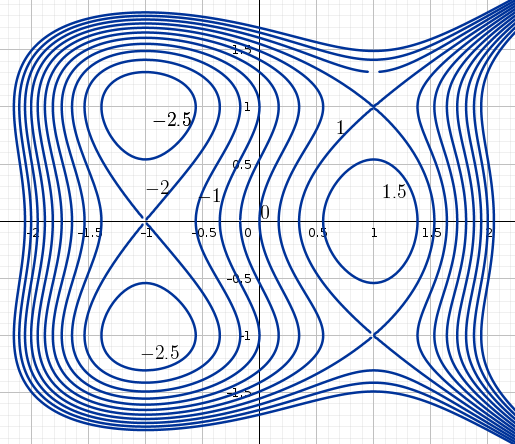
\includegraphics[width=0.4\linewidth]{images/lc-new} 

}

\caption{Level curves of an unknown function}\label{fig:unnamed-chunk-16}
\end{figure}

\end{exercise}

\begin{solution}

The graph suggests that the function has six critical points.

\begin{itemize}
\tightlist
\item
  We conclude that \((-1,1)\) and \((-1,-1)\) are local minimum points since the values of \(f\) appear to decrease as we approach these points from all possible directions.
\item
  We conclude that \((0,1)\) is a local maximum point since the values of \(f\) appear to increase as we approach this point from all possible directions.
\item
  We conclude that \((-1,0)\), \((1,1)\), and \((1,-1)\) are saddle points since the values of \(f\) can increase or decrease as we approach these points depending on the direction we choose. For example, if we approach point \((-1,0)\) from below, then the function values appear
  to decrease from \(1.5\) to \(1\), but if we approach from the left, then the function values appear to increase from \(0\) to \(1\).
\end{itemize}

\end{solution}

\hypertarget{lec-9}{%
\chapter{Constrained Optimization}\label{lec-9}}

Text References: Course notes pp.~37-52 \& Rogawski 14.8, 15.1-15.2

\hypertarget{recap-7}{%
\section{Recap}\label{recap-7}}

Last time, we learned how to find and classify the critical points of a function \(f(x,y)\).

\begin{exercise}
\protect\hypertarget{exr:unlabeled-div-65}{}\label{exr:unlabeled-div-65}

Find and classify the critical points of \(f(x,y)=(x^2+y^2)e^{-x}\).

\end{exercise}

\begin{solution}

To find the critical points, we calculate the gradient of the function and set it equal to zero:
\begin{align*}
\nabla f (x,y) &= (e^{-x}(2x-x^2-y^2), 2ye^{-x})=(0,0) \\
& \implies  e^{-x}(2x-x^2-y^2)=0 \quad\mbox{(1)}\quad \mbox{and} \quad 2ye^{-x}=0\quad\mbox{(2)}
\end{align*}
From \((2)\), we get \(y=0\). Substituting into \((1)\), we find \(e^{-x}(2x-x^2)=0\) which has solutions \(x=0\) and \(x=2\).

Therefore, the critical points are \((0,0)\) and \((2,0)\).

Next, we use the Second Derivative Test to classify the points. We have \[Hf(x,y)=\begin{bmatrix}e^{-x}(2-4x+x^2+y^2) & 2e^{-x}\\2e^{-x} & -2ye^{-x}\end{bmatrix}\]

Evaluating at \((0,0)\) and taking the determinant, we find \((2)(2)-0^2=4 >0\). Since \(f_{xx}=2>0\), we have a local minimum.

Evaluating at \((2,0)\) and taking the determinant, we find \((-2e^{-2})(2e^{-2}-0^2)=-4e^{-4}<0\), so we have a saddle point.

\end{solution}

\hypertarget{learning-objectives-8}{%
\section{Learning Objectives}\label{learning-objectives-8}}

\begin{itemize}
\tightlist
\item
  Given a function of several variables, use the Method of Lagrange to find its local extrema subject to a constraint \(g(x,y)=K\).
\end{itemize}

\hypertarget{method-of-lagrange}{%
\section{Method of Lagrange}\label{method-of-lagrange}}

It's common to want to find the local extrema of a function \(f(x.y)\) subject to a constraint. The most general way to express such a constraint is by defining a curve \(g(x,y)=K\). Let's think for a moment about what we're after. When we were finding the extrema of a function without constraints, we were looking for points \((a,b)\) where \(\nabla f (a,b)=0\). Now that we have constraints, it's possible that these points \((a,b)\) are not along the constraint curve, so we need to come up with a different idea.

What we're looking for are points along the constraint curve where \emph{infinitesimal movements in any direction don't result in either an increase or a decrease in the gradient of the function}. This is the type of behaviour we expect from the extrema of a function: at a max, for example, there's no direction in which we can move to increase the function.

Another way to say this is that we want points \((c,d)\) at which the directional derivative in the direction tangent to the constraint curve is equal to zero, i.e.\(D_{\vec{u}}(c,d)=\nabla f(c,d)\cdot\vec{u} =0\). This is a dot product, which means that the vector \(\vec{u}\) is orthogonal to \(\nabla f\).

Let's make one last observation: if we think of the constraint curve as being a particular level curve of some function \(g(x,y)\), then \(\nabla g\) will always be orthogonal to the constraint curve. This means that when \(\vec{u}\) is orthogonal to \(\nabla f\), it is also orthogonal to \(\nabla g\), so \(\nabla f\) and \(\nabla g\) are parallel, that is, \(\nabla f = \lambda \nabla g\) for some \(\lambda \in\mathbb{R}\).

An interactive example is shown in this \href{https://www.geogebra.org/m/wkkdvhqv}{applet}. The level curves of a function are given along with a constraint curve. Use the checkboxes to display \(\nabla f\) and \(\nabla g\). Observe the points at which the direction of the tangent at \(A\) is orthogonal to \(\nabla f\): how is \(\nabla g\) behaving at these points?

We have one final thing to consider: What if \(\nabla g=\vec{0}\) at some point on the constraint curve? This means that the constraint curve \(g(x,y)\) has a critical point. We need to check the value at this point, since we can't be sure whether they are actually extrema.

Putting all of what we've gathered together, we have the \textbf{Method of Lagrange}:

\begin{theorem}
\protect\hypertarget{thm:unlabeled-div-67}{}\label{thm:unlabeled-div-67}

To find the critical points of \(f(x,y)\) subject to a constraint \(g(x,y)=K\) for some constant \(K\), we must find the values of \(x\) and \(y\) for which:

\begin{enumerate}
\def\labelenumi{\arabic{enumi}.}
\tightlist
\item
  \(\nabla f(x,y)=\lambda \nabla g(x,y)\) and \(g(x,y)=K\) for some constant \(\lambda\); or
\item
  \(\nabla g(x,y)=(0,0)\) and \(g(x,y)=K\)
\end{enumerate}

\end{theorem}

A few notes on applying the Method of Lagrange:

\begin{itemize}
\tightlist
\item
  If the constraint is not given in the form \(g(x,y)=K\), we must rewrite it in that form
\item
  The proportionality constant \(\lambda\) is called a \textbf{Lagrange multiplier} and can be interpreted as the rate of change of \(f\) with respect to changes in the constraint value. In other words, \(\lambda\) is the additional \(f\) that is obtained by relaxing the constraint
  by \(1\) unit.
\item
  We can extend this method to functions of more than two variables and for problems with multiple constraints.
\item
  This method is used to \emph{locate} critical points, and not to classify them. In order to classify the critical points, we must evaluate the function at those points and compare values. Depending on the type of constraint curve, we distinguish two cases:

  \begin{enumerate}
  \def\labelenumi{\arabic{enumi}.}
  \tightlist
  \item
    If the constraint curve is closed (i.e.~has no endpoints), then we also need to consider the limits of \(f(x,y)\) in the two directions along the curve to determine whether we have any extrema.
  \item
    If the constraint curve has endpoints, we must also calculate the values of \(f(x,y)\) at those endpoints.
  \end{enumerate}
\end{itemize}

\begin{exercise}
\protect\hypertarget{exr:unlabeled-div-68}{}\label{exr:unlabeled-div-68}

Find the maximum value of \(6x+4y-7\) subject to \(3x^2+y^2=28\).

\end{exercise}

\begin{solution}

We have \(f(x,y)=6x+4y+7\) and so \(\nabla f (x,y)= (6, 4)\). We also have \(g(x,y)=3x^2+y^2\) and so \(\nabla g(x,y) = (6x, 2y)\).

\begin{enumerate}
\def\labelenumi{\arabic{enumi}.}
\tightlist
\item
  We find the points at which \(\nabla f(x,y)=\lambda \nabla g(x,y)\) and \(g(x,y)=28\). This gives us the following system:
  \begin{align*}
  6 &=  6 \lambda x \quad \mbox{(1)}\\
  4 &=  2 \lambda y \quad \mbox{(2)}\\
  3x^2+y^2 &=  28 \quad \mbox{(3)}\\
  \end{align*}
\end{enumerate}

Equation (1) tells us that \(x\neq 0\), so we can solve for \(\lambda\) to get \(\lambda=\frac{1}{x}\).

Substituting \(\lambda=\frac{1}{x}\) into equation (2), we find \(y=2x\); substituting that into equation (3) and solving for \(x\) gives \(x=\pm2\). When \(x=2\), we get \(y=4\); when \(x=-2\), we get \(y=-4\).

Therefore the critical points are \((2,4)\) and \((-2,-4)\).

\begin{enumerate}
\def\labelenumi{\arabic{enumi}.}
\setcounter{enumi}{1}
\tightlist
\item
  We check the points at which \(\nabla g = (0,0)\) and \(g(x,y)=28\).
\end{enumerate}

We have \(\ \nabla g(x,y)=(6x, 2y)\), which is equal to \((0,0)\) when \(x=y=0\); however, \(g(0,0)\neq 28\) so this point does not satisfy the constraint. Therefore, there are no critical points in this step.

Finally, we must evaluate \(f(x,y)\) at the critical points found above: \[f(2,4)=21 \quad \mbox{and} \quad f(-2,-4)=-35\]
Therefore, the maximum values of \(f(x,y)\) on the constraint curve is \(21\) and occurs at the point \((2,4)\).

This \href{https://www.geogebra.org/m/ruehzamn}{interactive applet} shows the level curves of \(f(x,y)\) are shown along with the constraint curve. Click and drag the point along the constraint curve to determine at which points \(f\) reaches its maximum or its minimum on the curve. Observe what happens to the gradients of \(f\) and \(g\) at these points.

\end{solution}

\hypertarget{lec-10}{%
\chapter{Double Integrals and Double Integrals Over Rectangles}\label{lec-10}}

Text References: Course notes pp.~37-52 \& Rogawski 14.8, 15.1-15.2

\hypertarget{recap-8}{%
\section{Recap}\label{recap-8}}

Last time, learned how to apply the Method of Lagrange to find the extrema of a function \(f(x,y)\) subject to a constraint \(g(x,y)=K\).

\begin{exercise}
\protect\hypertarget{exr:unlabeled-div-70}{}\label{exr:unlabeled-div-70}

Consider the level curves of a function \(f (x, y)\) and the constraint curve \(g(x, y) = k\) (in red). Estimate the maximum and minimum values of \(f\) with constraint \(g(x, y) = k\).

\begin{figure}

{\centering 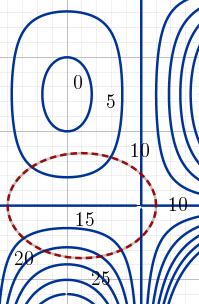
\includegraphics[width=0.3\linewidth]{images/lc-dashed-2} 

}

\caption{Level curves of an unknown function and constraint curve $g(x,y)=K$}\label{fig:unnamed-chunk-17}
\end{figure}

\end{exercise}

\begin{solution}

We check which level curves intersect with the constraint curve. We estimate that the maximum value is approximately \(24\) (between \(20\) and \(25\), but closer to \(25\) and the minimum value is approximately \(2\) (between \(0\) and \(5\), around halfway in between).

\end{solution}

\hypertarget{learning-objectives-9}{%
\section{Learning Objectives}\label{learning-objectives-9}}

\begin{itemize}
\tightlist
\item
  Given a function of several variables, integrate it with respect to a chosen variable.
\item
  Evaluate iterated integrals over rectangular domains
\end{itemize}

\hypertarget{partial-integration}{%
\section{Partial Integration}\label{partial-integration}}

In the past few weeks, we've been working on generalizing ideas from differential calculus; now, we're going to focus on integral calculus for a little bit.

Just like partial differentiation, we have a concept of \textbf{partial integration}: we can take the partial integral of a function of several variables by treating the variable of integration normally and any other variables as constants. The differential tells us which variable is the variable of integration.

\begin{exercise}
\protect\hypertarget{exr:unlabeled-div-72}{}\label{exr:unlabeled-div-72}

Calculate \(\displaystyle \int (2x+3y^2)dy\).

\end{exercise}

\begin{solution}

The differential is \(dy\), which means that \(y\) is the variable of integration. Treating \(x\) as a constant, we get
\[\displaystyle \int (2x+3y^2)dy  = 2xy + y^3 + g(x)\]

Note that instead of a constant \(C\), we have a \emph{function} \(g(x)\): since our variable of integration is \(y\), any function of \(x\) will disappear when we take the partial derivative with respect to \(y\).

\end{solution}

Partial integration can help us identify a function (up to a constant) if we know its partial derivatives.

\begin{exercise}
\protect\hypertarget{exr:unlabeled-div-74}{}\label{exr:unlabeled-div-74}

Find \(f(x,y)\) up to a constant if \(f_{x}(x,y)=4x^3y^3+3y^2+1\) and \(f_y = 3x^4y^2+6xy\).

\end{exercise}

\begin{solution}

Using partial integration, we have \[f(x,y)=\displaystyle \int f_xdx = \int (4x^3y^3+3y^2+1) dx =x^4y^3+3xy^2+x+g(y)\] and also \[f(x,y)=\displaystyle \int f_ydy = \int (3x^4y^2+6x)y dy = x^4y^3+3xy^2+h(x)\]

Putting it all together, we have \[f(x,y)=x^4y^3+3xy^2+x+g(y) \quad \mbox{and} \quad f(x,y)=x^4y^3+3xy^2+h(x)\]

Since the expressions are equal, this implies that \(x+g(y)=h(x)\); it must be that \(g(y)=C\) for some constant \(C\). Therefore, \(f(x,y)=x^4y^3+3xy^2+x+C\).

\end{solution}

\hypertarget{double-integrals}{%
\section{Double Integrals}\label{double-integrals}}

Until now, we've been doing a form of antidifferentiation; now, we're going to work on defining double integrals.

To start, we'll assume that the domain of integration is rectangular, that is, \(a\leq x\leq b\) and \(c\leq y\leq d\), and that \(f>0\) everywhere in this domain.

We can partition the region along the \(x\)-axis into \(m\) intervals of length \(\Delta x=\frac{(b-a)}{m}\); likewise, we can partition the region along the \(y\)-axis into \(n\) intervals of length \(\Delta y = \frac{(d-c)}{n}\). We've now partitioned the domain into rectangles with area \(\Delta A=\Delta x\Delta y\).

In each rectangle, we choose a point \((x_i^*, y_j^*)\). Then \(f(x_i^*, y_j^*)\Delta A\) represents the volume below the surface \(z=f(x,y)\) over the rectangle. Summing all of these volumes gives us an approximation of the volume below the surface over the domain. We also expect that as \(\Delta A\to 0\), the error in the approximation of the volume should approach zero. This motivates the following definition:

\begin{definition}
\protect\hypertarget{def:unlabeled-div-76}{}\label{def:unlabeled-div-76}

The \textbf{double integral} of a continuous function \(f(x,y)\) over a rectangular region \(R\in \mathbb{R}^2\) is \[\displaystyle \int_R f(x,y)dA =\lim_{m, n \to \infty}\sum_{i=1}^m\sum_{j=1}^nf(x_i^*, y_j^*)\Delta A\]

\end{definition}

This \href{https://www.geogebra.org/m/mcyzpeeh}{interactive applet} gives some intuition for what's happening in 3D space.

\hypertarget{double-integrals-over-rectangles}{%
\section{Double Integrals Over Rectangles}\label{double-integrals-over-rectangles}}

Rectangles are particularly nice domains over which to integrate: we can evaluate such integrals by performing partial integration of one variable at a time. The intuition for this is that when we fix one of the variables, we are singling out the cross-section of \(z=f(x,y)\) along that constant plane and calculating the area below this curve. Now, sweeping along the other variable, we give our cross-section slice some thickness and create a volume. A more detailed explanation of this can be found in the course notes.

From this intuition, we get the following result: If \(R=[a,b]\times[c,d]\), then \[\displaystyle \int_R f(x,y) dA=\int_c^d \int_a^b f(x,y) dx dy = \int_a^b \int_c^d f(x,y) dy dx\]

Notice that for these types of integrals, the order of integration doesn't matter! Unfortunately, this isn't always the case; it's one of the reasons we like integrating over rectangles so much. Given that the order of integration doesn't matter, this gives us a bit of freedom in deciding which order of integration works best.

Another nice property of integrals over rectangles is that if the integrand can be factored into a function of \(x\) and a function of \(y\), then the entire integral can be factored into an integral in \(x\) and an integral in \(y\). More formally, suppose that \(f(x,y)=g(x)h(y)\), then \[\displaystyle \int_c^d\int_a^b f(x,y) dxdy = \displaystyle \int_c^d\int_a^b g(x)h(y) dxdy=\displaystyle \int_c^dh(y)dy\int_a^b g(x) dx\]

\begin{exercise}
\protect\hypertarget{exr:unlabeled-div-77}{}\label{exr:unlabeled-div-77}

Evaluate \(\displaystyle \int_2^4 \int_1^9 ye^x dy dx\).

\end{exercise}

\begin{solution}

Note that we first integrate with respect to \(y\) and the with respect to \(x\):
\begin{align*}
\displaystyle \int_2^4 \int_1^9 ye^x dy dx & = \int_2^4 \left ( \int_1^9 ye^x dy \right )dx\\
&= \int_2^4 \left (e^x\int_1^9 y dy\right ) dx\\
&= \int_2^4 \left ( \dfrac{e^xy^2}{2}\right |_{y=1}^9 dx\\
&= \int_2^4 40e^x dx\\
&= 40(e^4-e^2)
\end{align*}

\end{solution}

\begin{exercise}
\protect\hypertarget{exr:unlabeled-div-79}{}\label{exr:unlabeled-div-79}

Evaluate \(\displaystyle \int_0^{1}\int_{-\pi}^{\pi}x\sin(xy)dx dy\).

\end{exercise}

\begin{solution}

We notice that in this case, it's much, \emph{much} simpler to integrate first with respect to \(y\), then with respect to \(x\):
\begin{align*}
\displaystyle \int_0^1\int_{-\pi}^{\pi}x\sin(xy)dx dy & = \displaystyle \int_{-\pi}^{\pi}\int_{0}^1x\sin(xy)dy dx\\
& = \displaystyle \int_{-\pi}^{\pi} \left (x \int_0^1 \sin(xy)dy \right)dx \\
& = \displaystyle \int_{-\pi}^{\pi}  \left  (\dfrac{-x\cos(xy)}{x} \right|_{y=0}^1 dx \\
& = \displaystyle \int_{-\pi}^{\pi} -\cos(x)+\cos(0) dx \\
&= \left . -\sin(x) \right |_{x=-\pi}^{\pi}+ \left. x\cos(0) \right|_{x=-\pi}^{\pi}\\
&= 2\pi
\end{align*}

\end{solution}

\hypertarget{lec-11}{%
\chapter{Double Integrals Over Non-Rectangular Domains}\label{lec-11}}

Text References: Course notes pp.~37-52 \& Rogawski 14.8, 15.1-15.2

\hypertarget{recap-9}{%
\section{Recap}\label{recap-9}}

Last time, we worked with double integrals over rectangular domains.

\begin{exercise}
\protect\hypertarget{exr:unlabeled-div-81}{}\label{exr:unlabeled-div-81}

Find the volume \(V\) of the solid enclosed between the graph of \(f(x,y)=16-x^2-3y^2\) and the rectangle \(R=[0,3]\times [0,1]\).

\end{exercise}

\begin{solution}

The volume of the solid is given by the double integral of \(f(x,y)\), which we can write as the following iterated integral: \[V=\displaystyle \iint_R (16-x^2-3y^2)dA = \int_0^3\int_0^1 (16-x^2-3y^2)dy dx\]

Evaluating the integral, we get
\begin{align*}
\int_0^3\int_0^1 (16-x^2-3y^2)dy dx & = \int_0^3 \left (16y-x^2y-y^3 \right|_{y=0}^1 dx \\
&= \int_0^3 15-x^2 dx \\
&= \left . 15x-\dfrac{1}{3}x^3\right|_{x=0}^3 \\
&= 36
\end{align*}

\end{solution}

\hypertarget{learning-objectives-10}{%
\section{Learning Objectives}\label{learning-objectives-10}}

\begin{itemize}
\tightlist
\item
  Given a region, classify it as Type I, Type II, or Type III.
\item
  Evaluate integrals over non-rectangular domains
\end{itemize}

\hypertarget{double-integrals-over-non-rectangular-domains}{%
\section{Double Integrals Over Non-Rectangular Domains}\label{double-integrals-over-non-rectangular-domains}}

Today, we're going to work on integrating over types of regions which cannot be described as rectangles. We distinguish three types of region.

\hypertarget{type-i-regions}{%
\subsection{Type I Regions}\label{type-i-regions}}

A \textbf{Type I} region is one which can be described as lying between the graphs of two functions of \(x\) over some interval. That is, we have \(a\leq x\leq b\) and \(g(x)\leq y\leq h(x)\). In this case, we have \[\displaystyle \int_R f(x,y)dA = \int_a^b \int_{g(x)}^{h(x)}f(x,y) dy dx\]

\begin{figure}

{\centering 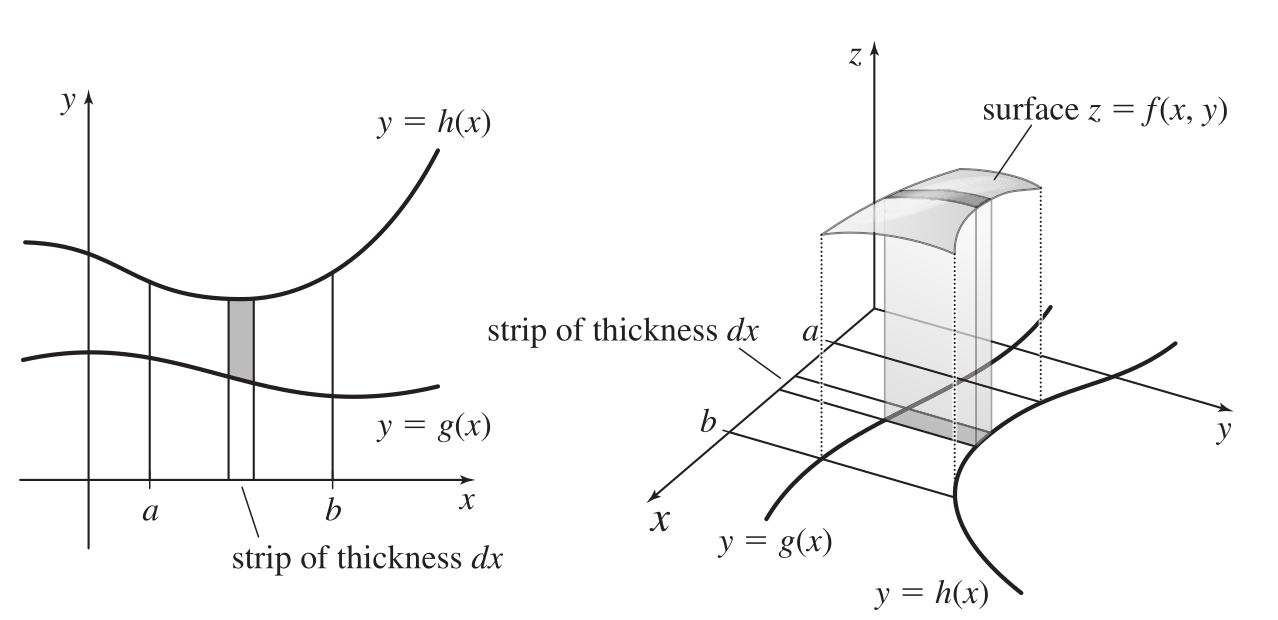
\includegraphics[width=0.75\linewidth]{images/type-i} 

}

\caption{Type I regions}\label{fig:unnamed-chunk-18}
\end{figure}

\hypertarget{type-ii-regions}{%
\subsection{Type II Regions}\label{type-ii-regions}}

A \textbf{Type II} region is one which can be described as lying between the graphs of two functions of \(y\) over some interval. That is, we have \(c\leq y\leq d\) and \(g(y)\leq x\leq h(y)\). In this case, we have \[\displaystyle \int_R f(x,y)dA = \int_c^d \int_{g(y)}^{h(y)}f(x,y) dx dy\]

\begin{figure}

{\centering 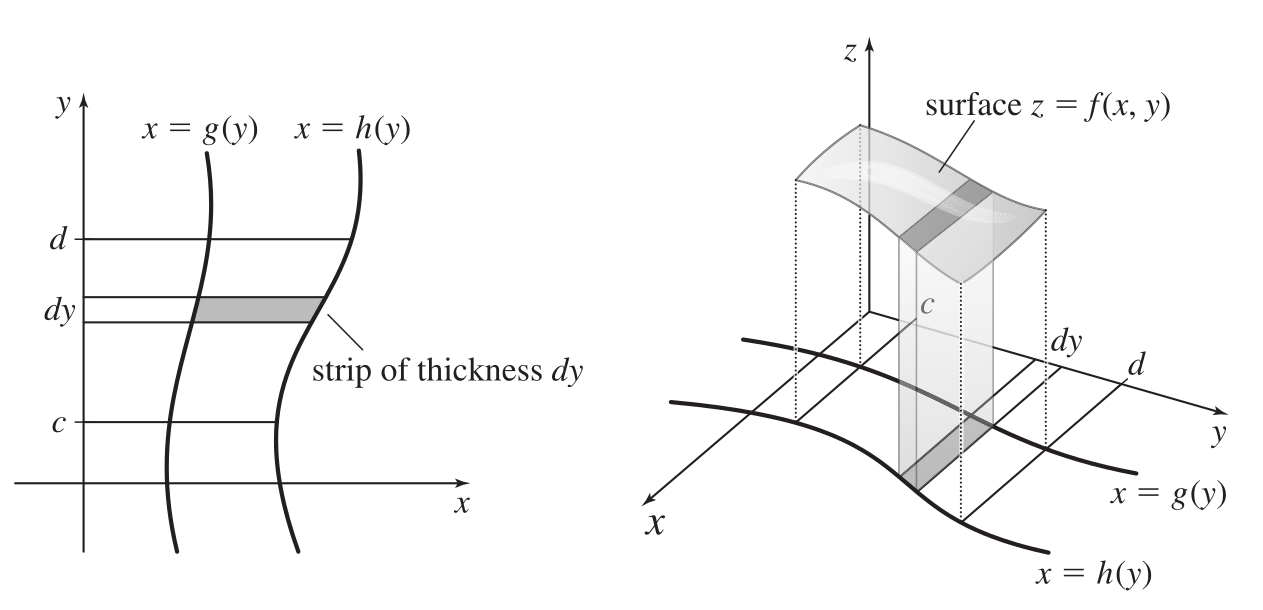
\includegraphics[width=0.75\linewidth]{images/type-ii} 

}

\caption{Type II regions}\label{fig:unnamed-chunk-19}
\end{figure}

\hypertarget{type-iii-regions}{%
\subsection{Type III Regions}\label{type-iii-regions}}

A \textbf{Type III} region is one that is neither Type I not Type II. Our approach in this case is to subdivide the region into smaller regions which are of one type or the other.

\hypertarget{exercises}{%
\section{Exercises}\label{exercises}}

A good strategy for solving problems involving integration over non-rectangular domains is to start by sketching the region, identifying its type, and then setting up and solving the integral.

\begin{exercise}
\protect\hypertarget{exr:unlabeled-div-83}{}\label{exr:unlabeled-div-83}

Evaluate \(\displaystyle \iint_R xy dA\) where \(R\) is the triangular region with vertices \((0,0)\), \((2,0)\), and \((0,1)\).

\end{exercise}

\begin{solution}

Let's start by sketching the region. Note that we can set this up either as a Type I or Type II region.

Let's classify it as Type I to start:

\begin{figure}

{\centering 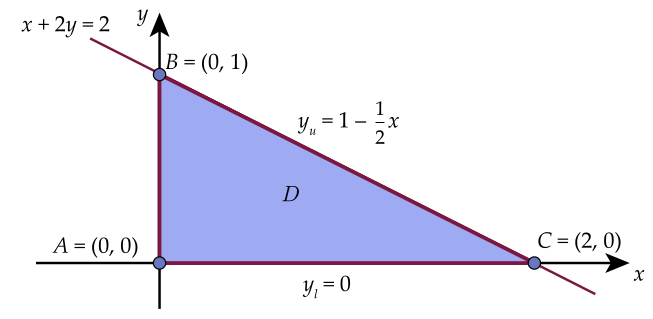
\includegraphics[width=0.75\linewidth]{images/lec-11-1} 

}

\caption{Sketch of $R$}\label{fig:unnamed-chunk-20}
\end{figure}

The region \(R\) can be described by \[0\leq x \leq 2 \quad \mbox{and}\quad 0\leq y\leq 1-\dfrac{1}{2}x\]

Writing the integral, we get

\begin{align*}
\displaystyle \iint_R xy dA & = \int_0^2\int_0^{1-\frac{1}{2}x}xy dy dx \\
&= \int_0^2 x\left (\dfrac{y^2}{2}\right |_{y=0}^{1-\frac{1}{2}x} dx\\
&= \dfrac{1}{2}\int_0^2 x\left (1-\dfrac{1}{2}x \right)^2 dx\\
&= \left ( \dfrac{x^2}{4}-\dfrac{1}{6}x^3+\dfrac{1}{32}x^4 \right|_{0}^2\\
&=\dfrac{1}{6}
\end{align*}

If, instead, we set this up as a Type II integral, we might change our sketch as follows:

\begin{figure}

{\centering 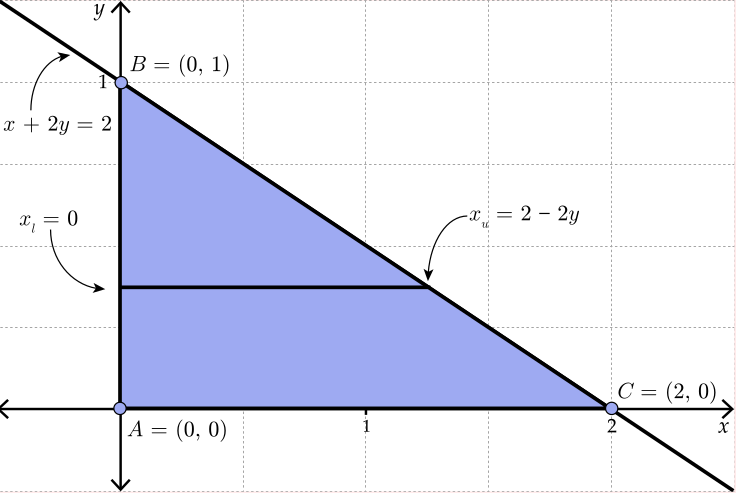
\includegraphics[width=0.75\linewidth]{images/lec-11-2} 

}

\caption{Sketch of $R$}\label{fig:unnamed-chunk-21}
\end{figure}

The region \(R\) can be described by \[0\leq y\leq 1 \quad \mbox{and}\quad 0\leq x \leq 2-2y\]

Writing the integral, we get

\begin{align*}
\displaystyle \iint_R xy dA & = \int_0^1\int_0^{2-2y}xy dx dy \\
&= \int_0^1 y \left (\dfrac{x^2}{2}\right |_{x=0}^{2-2y} dy\\
&= 2\int_0^1 y(1-y)^2 dy\\
&=\dfrac{1}{6}
\end{align*}

\end{solution}

\begin{exercise}
\protect\hypertarget{exr:unlabeled-div-85}{}\label{exr:unlabeled-div-85}

Evaluate \(\displaystyle \int_0^1\int_0^y e^{x^2}dxdy\).

\end{exercise}

\begin{solution}

Note that integrating first with respect to \(x\) is not to our advantage; we can change the order of integration (and also the bounds!) to simplify things.

The region is the triangle with vertices \((0,0)\), \((1,0)\), and \((1,1)\):

\begin{figure}

{\centering 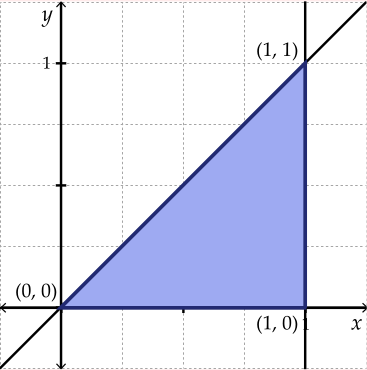
\includegraphics[width=0.3\linewidth]{images/lec-11-3} 

}

\caption{Sketch of $R$}\label{fig:unnamed-chunk-22}
\end{figure}

The region \(R\) can be described by \[0\leq x\leq 1 \quad \mbox{and}\quad 0\leq y \leq x\]

Writing the integral, we get

\begin{align*}
\displaystyle \iint_R e^{x^2} dA & = \int_0^1\int_0^{x}e^{x^2} dy dx \\
&= \int_0^1 y \left . e^{x^2}\right |_{y=0}^{x} dx\\
&= \int_0^1 xe^{x^2} dx\\
&=\dfrac{e-1}{2}
\end{align*}

\end{solution}

\begin{exercise}
\protect\hypertarget{exr:unlabeled-div-87}{}\label{exr:unlabeled-div-87}

Find the volume \(V\) of the region under the plane \(z=2x+3y\) and above the triangle shown in the figure below

\begin{figure}

{\centering 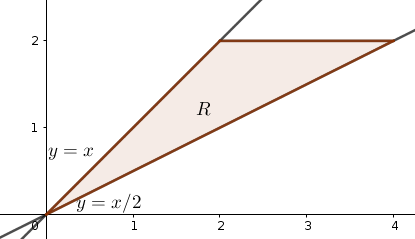
\includegraphics[width=0.3\linewidth]{images/lec-11-4} 

}

\caption{Sketch of $R$}\label{fig:unnamed-chunk-23}
\end{figure}

\end{exercise}

\begin{solution}

The simplest way to set up is integral is using a Type II region. Describing it as Type I is possible, but would require setting up two integrals instead of one (why?).

The region \(R\) can be described by \[0\leq y\leq 1 \quad \mbox{and}\quad y\leq x \leq 2y\]

Writing the integral, we get

\begin{align*}
\displaystyle \iint_R 2x+3y dA & = \int_0^2\int_y^{2y}2x+3y \, dx dy \\
&= \int_0^2 \left (x^2+3yx \right |_{x=y}^{2y} dy\\
&= \int_0^2 6y^2 dy \\
&= 16
\end{align*}

\end{solution}

\hypertarget{lec-12}{%
\chapter{Double Integrals in Polar Coordinates}\label{lec-12}}

Text References: Course notes pp.~53-65 \& Rogawski 11.3, 15.4-15.6

\hypertarget{recap-10}{%
\section{Recap}\label{recap-10}}

Last time, we worked with double integrals over non-rectangular domains.

\begin{exercise}
\protect\hypertarget{exr:unlabeled-div-89}{}\label{exr:unlabeled-div-89}

Use inequalities to describe the region pictured below:

\begin{figure}

{\centering 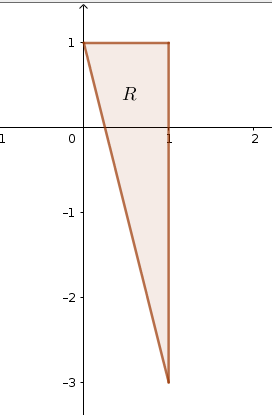
\includegraphics[width=0.3\linewidth]{images/lec-12-recap} 

}

\caption{Triangle in the $xy$-plane}\label{fig:unnamed-chunk-24}
\end{figure}

\end{exercise}

\begin{solution}

The region \(R\) can be described by \[-3\leq y \leq 1 \quad \mbox{and}\quad \dfrac{1-y}{4}\leq x\leq 1\] or by \[0\leq x\leq 1 \quad \mbox{and}\quad -4x+1\leq y \leq 0 \]

\end{solution}

\hypertarget{learning-objectives-11}{%
\section{Learning Objectives}\label{learning-objectives-11}}

\begin{itemize}
\tightlist
\item
  Evaluate integrals using polar coordinates.
\end{itemize}

\hypertarget{polar-coordinates}{%
\section{Polar Coordinates}\label{polar-coordinates}}

The techniques that we've seen so far for setting up and evaluating double integrals are not always suited for more complicated regions. We're going to start building up a key tool in our integration toolkit, starting with a discussion of polar coordinates.

Polar coordinates are particularly useful when the domain \(R\):

\begin{itemize}
\tightlist
\item
  is circular or has circles forming part of its boundary; and
\item
  contains the expression \(x^2+y^2\) (which will become \(\rho^2\) after changing to polar coordinates)
\end{itemize}

Recall that to convert from Cartesian coordinates to polar coordinates, we set \(x= \rho \cos(\phi)\) and \(y=\rho\sin(\phi)\).

\hypertarget{double-integrals-in-polar-coordinates}{%
\section{Double Integrals in Polar Coordinates}\label{double-integrals-in-polar-coordinates}}

The question now becomes how to transform our original integral \(\displaystyle \iint_R f(x,y)dA\) to polar coordinates. We can substitute \(x= \rho \cos(\phi)\) and \(y=\rho\sin(\phi)\) to get \(\displaystyle \iint_R f(x,y)dA = \iint_R f(\rho\cos(\phi), \rho\sin(\phi))dA\).

Recall that the area element \(dA\) in the original integral is thought of as the area of a rectangle: \(dA=dxdy\). Now that we've converted to polar coordinates, we need to adjust the area element.

In polar coordinates, we can partition the range of values of \(\rho\) into segments of equal length \(d\rho\); graphically, these are circles centred at the origin. We can also partition the values of \(\phi\) into small, equal angles \(d\phi\):

\begin{figure}

{\centering 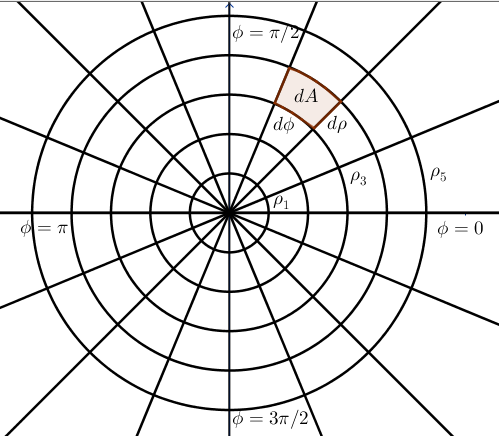
\includegraphics[width=0.5\linewidth]{images/lec-12-polar} 

}

\caption{Partitioning of the polar plane}\label{fig:unnamed-chunk-25}
\end{figure}

In order to find the area of \(dA\), recall that for a circle of radius \(r\), a sector of angle \(\theta\) has area \(\frac{r^2\theta}{2}\). Our sector is bounded above by \(\rho + d\rho\) and below by \(\rho\), so the area of the polar rectangle is the difference bewteen the area of the full sector of radius \(\rho + d\rho\) and the smaller sector of radius \(\rho\).

We get
\begin{align*}
dA &= \frac{1}{2}(\rho+d\rho)^2 d\phi- \frac{1}{2}\rho^2 d\phi\\
&= \rho~d\rho d\phi + \frac{1}{2} d\rho^2 d\phi
\end{align*}

Since \(d\phi\) and \(d\rho\) are infinitesimally small, we can ignore the square term. We can now express our original integral using polar coordinates as follows: \[\displaystyle \iint_{R_{xy}} f(x,y)dA = \iint_{R_{\rho \phi}} f(\rho\cos(\phi), \rho\sin(\phi)) \rho~d\rho d\phi\]

It is extremely important to notice (and not to forget!) the factor of \(\rho\) in the integral expressed in polar coordinates! Also, notice that the domain \(R_{\rho\phi}\) indicates that we must write the domain in polar coordinates.

\begin{exercise}
\protect\hypertarget{exr:unlabeled-div-91}{}\label{exr:unlabeled-div-91}

Evaluate \(\displaystyle \iint_R (3yx^2+3y^3)dA\) where \(R\) is the semicircle of radius \(2\) that starts in the first quadrant and ends in the second quadrant.

\begin{figure}

{\centering 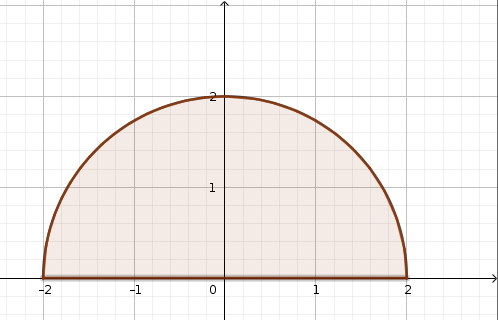
\includegraphics[width=0.3\linewidth]{images/lec-12-ex-1} 

}

\caption{Semicircle of radius 2}\label{fig:unnamed-chunk-26}
\end{figure}

\end{exercise}

\begin{solution}

To solve this problem, we can convert to polar coordinates by setting \(x=\rho\cos(\phi)\) and \(y=\rho\sin(\phi)\).

First, let's describe the domain \(R\). We can describe the semicircle using the inequalities \[0\leq \rho\leq 2 \quad\mbox{and}\quad 0\leq \phi\leq \pi\]

Next, we convert the integrand to polar coordinates: \[3yx^2+3y^3 = 3y(x^2+y^2) = 3\sin(\phi)\rho^2\]

Now, we can set up and solve the integral, taking care to remember the factor of \(\rho\):

\begin{align*}
\displaystyle \iint_R (3yx^2+3y^3)dA &= \int_{0}^{\pi}\int_0^2 3\sin(\phi)\rho^2~\rho~d\rho d\phi \\
&= \int_{0}^{\pi}\int_0^2 3\sin(\phi)\rho^3~d\rho d\phi \\
&= \int_0^{\pi}3\sin(\phi)\left (\frac{\rho^4}{4} \right|_{\rho=0}^2 d\phi\\
&= \int_0^{\pi}12\sin(\phi)d\phi\\
&= 24
\end{align*}

\end{solution}

\begin{exercise}
\protect\hypertarget{exr:unlabeled-div-93}{}\label{exr:unlabeled-div-93}

Evaluate \(\displaystyle \iint_R x dA\) over the region bounded between the semicircle of radius \(1\) and the semicircle of radius \(2\) that start in the fourth quadrant and end in the first quadrant.

\begin{figure}

{\centering 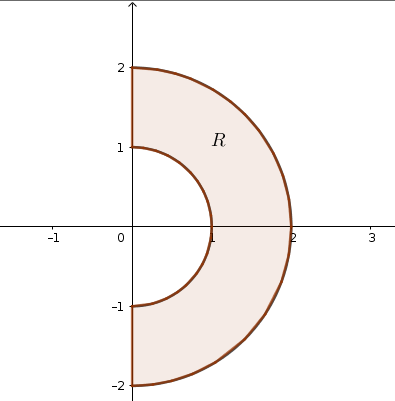
\includegraphics[width=0.3\linewidth]{images/lec-12-ex-2} 

}

\caption{Domain of integration}\label{fig:unnamed-chunk-27}
\end{figure}

\end{exercise}

\begin{solution}

First, let's describe the domain \(R\). We can describe the region using the inequalities \[1\leq \rho\leq 2 \quad\mbox{and}\quad {- 3\pi/2}\leq \phi\leq \pi/2\]

Next, we convert the integrand to polar coordinates: \[x =\rho\cos(\phi)\]

Now, we can set up and solve the integral, taking care to remember the factor of \(\rho\):

\begin{align*}
\displaystyle \iint_R x dA &= \int_{-3\pi/2}^{\pi/2}\int_1^2 \rho\cos(\phi)~\rho~d\rho d\phi \\
&= \int_{-3\pi/2}^{\pi/2}\int_1^2 \rho^2 \cos(\phi) d\rho d\phi\\
&= \int_{-3\pi/2}^{\pi/2}\cos(\phi) \int_1^2 \rho^2 d\rho d\phi \\
&= \int_{-3\pi/2}^{\pi/2}\cos(\phi) \left (\frac{\rho^3}{3}\right |_{\rho=1}^2\\
& = \int_{-3\pi/2}^{\pi/2} \frac{7}{3}\cos(\phi)\\
&= 0
\end{align*}

\end{solution}

\hypertarget{lec-13}{%
\chapter{The Change of Variable Formula}\label{lec-13}}

Text References: Course notes pp.~53-65 \& Rogawski 11.3, 15.4-15.6

\hypertarget{recap-11}{%
\section{Recap}\label{recap-11}}

Last time, we learned another technique for solving double integrals: changing to polar coordinates.

\begin{exercise}
\protect\hypertarget{exr:unlabeled-div-95}{}\label{exr:unlabeled-div-95}

Transform the integral \(\displaystyle \int_{-3}^0\int_{-\sqrt{9-y^2}}^{\sqrt{9-y^2}} 1~dxdy\) to polar coordinates (no need to solve the integral).

\end{exercise}

\begin{solution}

We are working with the inequalities \(-3\leq y\leq 0\) and \(-\sqrt{9-y^2}\leq x\leq \sqrt{9-y^2}\). We can rewrite the second inequality as \(x^2=9-y^2 \implies x^2+y^2=9\), which describes a circle of radius \(3\). The additional conditions on \(y\) mean that we are only considering the bottom half of the circle.

\begin{figure}

{\centering 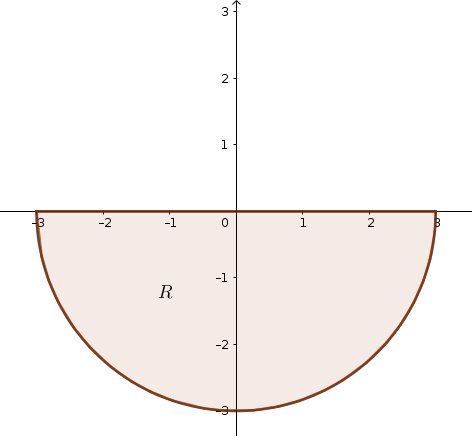
\includegraphics[width=0.3\linewidth]{images/lec-13-recap} 

}

\caption{Domain of integration}\label{fig:unnamed-chunk-28}
\end{figure}

Thus, \(0\leq \rho \leq 3\) and \(\pi\leq\phi\leq 2\pi\). Remembering the factor of \(\rho\) in the integrand, we get \[\int_{0}^3\int_{\pi}^{2\pi}\rho~d\rho d\phi\]

\end{solution}

\hypertarget{learning-objectives-12}{%
\section{Learning Objectives}\label{learning-objectives-12}}

\begin{itemize}
\tightlist
\item
  Evaluate integrals using the change of variables formula.
\end{itemize}

\hypertarget{transformations}{%
\section{Transformations}\label{transformations}}

Thinking back to our work with polar coordinates, we've seen that changing coordinates is in fact a \emph{transformation} which maps the \(xy\)-plane to the \(\rho\phi\)-plane. This is the idea we're going to try go generalize to help us solve integration problems: if the region of integration is not ``nice'', we can apply a transformation to it and turn it into a ``nice'' region that's easier to integrate over.

Let's think for a moment about which regions are particularly nice to integrate over: rectangles! Our goal in coming up with transformations will generally be to transform integrals over non-rectangular domains into integrals over rectangular domains (or, if that's not so straightforward, into regions of Type I or Type II). As with polar coordinates, we will have to think carefully about what the new area element \(dA\) should be.

\begin{exercise}
\protect\hypertarget{exr:unlabeled-div-97}{}\label{exr:unlabeled-div-97}

Find a mapping which transforms the region \(R_{xy}\) in the first quadrant bounded by the hyperbolae \(xy=1\), \(xy=3\), \(x^2-y^2=2\), \(x^2-y^2=4\) into a square in the \(uv\)-plane.

\end{exercise}

\begin{solution}

Take \(u(x,y)=xy\) and \(v(x,y)=x^2-y^2\). The boundaries of the region will map to the horizontal lines \(u=1\) and \(u=3\) and to the vertical lines \(v=2\) and \(v=4\) in the \(uv\)-plane.

\end{solution}

\hypertarget{the-change-of-variables-formula}{%
\section{The Change of Variables Formula}\label{the-change-of-variables-formula}}

Let's dive into the main result.

\begin{theorem}
\protect\hypertarget{thm:unlabeled-div-99}{}\label{thm:unlabeled-div-99}

Suppose that the variables \(x\) and \(y\) are related to the variables \(u\) and \(v\) by the equations \(x=x(u,v)\), \(y=y(u,v)\). Then, \[\iint_{R_{xy}}f(x,y)~dxdy = \iint_{R_{uv}}f(x(u,v), y(u,v)) \left |\dfrac{\partial(x,y)}{\partial (u,v)}\right|~dudv\]
where \[\dfrac{\partial(x,y)}{\partial (u,v)}=\det\begin{bmatrix}\frac{\partial x}{\partial u}&\frac{\partial x}{\partial v}\\ \frac{\partial y}{\partial u}& \frac{\partial y}{\partial v}\end{bmatrix}\] This function is called the \textbf{Jacobian} of the transformation, and is also denoted by \(J\). Note that \(\left |\dfrac{\partial(x,y)}{\partial (u,v)}\right|\) is the \emph{absolute value} of the determinant of the matrix of partial derivatives.

\end{theorem}

When applying the change of variables formula, it's important to keep a few things in mind:

\begin{itemize}
\tightlist
\item
  The transformation \((x,y)\to (u,v)\) must be invertible on the domain of integration. In other words, we can't have \(J=0\) at any point on the interior of \(R_{uv}\); we don't want to lose information by, for example, contracting a line to a point.
\item
  The Jacobian can be understood as area scaling factor of a given transformation. That is, the Jacobian describes the extent to which the associated mapping increases or decreases areas.
\item
  As we might expect, \(\dfrac{\partial(x,y)}{\partial(u,v)}=\dfrac{1}{\frac{\partial(u,v)}{\partial(x,y)}}\)
\end{itemize}

\begin{exercise}
\protect\hypertarget{exr:unlabeled-div-100}{}\label{exr:unlabeled-div-100}

Evaluate \(\displaystyle \iint_R x dA\) where \(R\) is the region in the first and fourth quadrants bounded by the curves \(y+x^2=0\), \(y+x^2=1\), \(y-x^2=0\), and \(y-x^2=-1\).

\end{exercise}

\begin{solution}

We start by defining a map that converts this region into the unit square in the \(uv\)-plane by setting \(u(x,y)=x+y^2\) and \(v(x,y)=y-x^2\).

Writing \(x\) and \(y\) in terms of \(u\) and \(v\), we can sum \(u\) and \(v\) to find \(y=\frac{u+v}{2}\); and we can subtract \(u\) and \(v\) to find \(x=\sqrt{\frac{u-v}{2}}\). Note that we have \(0\leq u\leq 1\) and \(0\leq v\leq 1\).

Next, we calculate the Jacobian:
\[\dfrac{\partial(x,y)}{\partial (u,v)}=\det\begin{bmatrix}\frac{\partial x}{\partial u}&\frac{\partial x}{\partial v}\\ \frac{\partial y}{\partial u}& \frac{\partial y}{\partial v}\end{bmatrix} = \begin{bmatrix}\frac{1}{2\sqrt{2u-2v}}& -\frac{1}{2\sqrt{2u-2v}}\\ \frac{1}{2} & \frac{1}{2}\end{bmatrix} = \dfrac{1}{2\sqrt{2u-2v}}\]

Now, we express the integrand in terms of the new variables: \(x=\sqrt{\frac{u-v}{2}}\).

Putting everything together, we apply the change of variables: \[ \iint_R x dA = \int_0^1\int_0^1 \frac{1}{2\sqrt{2u-2v}}\sqrt{\frac{u-v}{2}}du dv = \int_0^1\int_0^1 \frac{1}{4} du dv = \frac{1}{4}\]

\end{solution}

\begin{exercise}
\protect\hypertarget{exr:unlabeled-div-102}{}\label{exr:unlabeled-div-102}

Evaluate \(\displaystyle \iint_R (x^2-xy -y^2) dA\) where \(R\) is the region in the first quadrant bounded by the hyperbolae \(xy=1\), \(xy=3\), \(x^2-y^2=2\), \(x^2-y^2=4\) into a square in the \(uv\)-plane.

\end{exercise}

\begin{solution}

Using the transformation we found in an earlier example, we have \(u(x,y)=xy\) and \(v(x,y)=x^2-y^2\). Note that in this case, writing \(x\) and \(y\) in terms of \(u\) and \(v\) is not so simple; we will use the property of the Jabobian that \(\dfrac{\partial(x,y)}{\partial(u,v)}=\dfrac{1}{\frac{\partial(u,v)}{\partial(x,y)}}\).

\[\frac{\partial(u,v)}{\partial(x,y)} = \det \begin{bmatrix}\frac{\partial u}{\partial x}&\frac{\partial u}{\partial y}\\ \frac{\partial v}{\partial x}& \frac{\partial v}{\partial y}\end{bmatrix}=\det\begin{bmatrix}y & x\\2x& -2y\end{bmatrix}=-2y^2-2x^2\]

and so \[\dfrac{\partial(x,y)}{\partial(u,v)}=\dfrac{1}{\frac{\partial(u,v)}{\partial(x,y)}} = \frac{1}{-2y^2-2x^2}\]

Expressing the integrand in terms of the new variables, we get \[x^2-xy -y^2 = v-u\]

\end{solution}

\hypertarget{lec-14}{%
\chapter{Applications of Multiple Integrals}\label{lec-14}}

Text References: Course notes pp.~53-65 \& Rogawski 11.3, 15.4-15.6

\hypertarget{recap-12}{%
\section{Recap}\label{recap-12}}

Last time, we rounded out our toolkit for evaluating double integrals with the change of variables formula.

\begin{exercise}
\protect\hypertarget{exr:unlabeled-div-104}{}\label{exr:unlabeled-div-104}

Consider the change of variables \(x=3u+v\) and \(y=u-2v\). Determine the area of the rectangle \(R=[2,5]\times[1,7\) under this transformation.

\end{exercise}

\begin{solution}

In order to determine the area scaling factor, we need to calculate the Jacobian of the transformation. We have

\begin{align*}
\dfrac{\partial(x,y)}{\partial(u,v)}&=\det\begin{bmatrix}\frac{\partial x}{\partial u} & \frac{\partial x}{\partial v} \\
\frac{\partial y}{\partial u}& \frac{\partial y}{\partial v}\end{bmatrix} \\
&=\det \begin{bmatrix}3& 1\\ 1&-2\end{bmatrix}\\
&= -7
\end{align*}

Taking the absolute value, we get a scaling factor of \(7\). The area of the rectangle is \(3\cdot 6=18\) square units; multiplying by the scaling factor, we get \(126\) square units.

\end{solution}

\hypertarget{learning-objectives-13}{%
\section{Learning Objectives}\label{learning-objectives-13}}

\begin{itemize}
\tightlist
\item
  Explain several applications of integrals.
\end{itemize}

\hypertarget{applications-of-double-integrals}{%
\section{Applications of Double Integrals}\label{applications-of-double-integrals}}

Until now, we have mainly focused on interpreting integrals as either areas under curves (for single integrals) or volumes under surfaces (for double integrals). Today, we're going to broaden our interpretation of integrals to include other types of applications.

\hypertarget{definite-integrals}{%
\subsection{Definite Integrals}\label{definite-integrals}}

Let's take a look at the formal definition of a definite integral: \[\int_a^b f(x) dx = \lim_{n\to\infty}\sum_{i=1}^nf(x_i^*)\Delta x\]
where \(x_i^*\in[x_{i-1}, x_i]\) and \([a,b]\) is divided into \(n\) sub-intervals of equal width \(\Delta x\).

The interpretation of this integral hinges on our interpretation of \(f(x)\) and \(x\). So far, we've been interpreting \(\Delta x\) and \(f(x_i^*)\) as the width and height of a small rectangle, which means that the result of the integral is an area.

Let's take a look at other possible interpretations.

\begin{example}
\protect\hypertarget{exm:unlabeled-div-106}{}\label{exm:unlabeled-div-106}

If \(t\) measures time (s) and \(f(t)\) measures velocity (m/s) in a straight line, then \(\displaystyle \int_a^b f(t) dt\) is a sum of infinitesimal displacements \(ds=f(t) dt\). The integral therefore represents the \emph{total displacement} of a particle moving with velocity \(f(t)\) between \(t=a\) and \(t=b\).

\end{example}

\begin{example}
\protect\hypertarget{exm:unlabeled-div-107}{}\label{exm:unlabeled-div-107}

Consider a charged rod of length \(L\). If \(x\) measures the distance (meters) from one end of the rod and \(\rho (x)\) is the linear charge density in the rod (coulombs/meter), then \(\displaystyle \int_0^L \rho(x) dx\) gives the total charge of the rod.

\end{example}

\begin{example}
\protect\hypertarget{exm:unlabeled-div-108}{}\label{exm:unlabeled-div-108}

If \(f(x,y)\) is a population density (organisms/km\(^2\)) and \(R\) is a region, then \(\displaystyle \iint_R f(x,y)dA\) gives the total population within the region \(R\).

\end{example}

\begin{example}
\protect\hypertarget{exm:unlabeled-div-109}{}\label{exm:unlabeled-div-109}

The average value of a function \(f(x,y)\) over a two-dimensional region \(R\) can be calculated as \(\displaystyle f_{avg}=\frac{1}{\mbox{Area}(R)}=\iint_R f(x,y)dA\).

\end{example}

\begin{exercise}
\protect\hypertarget{exr:unlabeled-div-110}{}\label{exr:unlabeled-div-110}

The population in a rural area has density \(\delta(x,y)=40xe^{0.1y}\) people per km\(^2\). How many people live in the region \(R: 2\leq x \leq 6, 1\leq y\leq 3\)?

\end{exercise}

\begin{solution}

The population in the region \(R\) is given by the integral of the population density:

\begin{align*}
\displaystyle \iint_R 40xe^{0.1y} dA & = \int_1^3 \int_2^6 40xe^{0.1y} dxdy\\
&= \int_1^3 \left (20x^2e^{0.1y}\right |_{x=2}^6)dy \\
&= \int_1^3 640 e^{0.1y}dy\\
&= \left . 6400 e^{0.1y}\right |_{y=1}^3\\
& \approx 1566 \, \mbox{people}
\end{align*}

\end{solution}

\hypertarget{integrals-with-no-integrand}{%
\subsection{Integrals with no Integrand}\label{integrals-with-no-integrand}}

Thinking back to single-variable calculus, the integral \(\displaystyle \int_a^b dx\) is the length of the interval of integration \([a,b]\): \(\displaystyle \int_a^b dx=b-a\). A similar interpretation holds for double integrals: \(\displaystyle \iint_R dA\) is the area of the domain \(R\).

\begin{exercise}
\protect\hypertarget{exr:unlabeled-div-112}{}\label{exr:unlabeled-div-112}

Find the area of the region \(R\) bounded by the curves \(y=x\) and \(y=x^2\).

\end{exercise}

\begin{solution}

Note that the curves intersect at \((0,0)\) and \((1,1)\). One way to describe the region is \(0\leq x \leq 1\) and \(x^2\leq y \leq x\). The area of the region is therefore given by

\begin{align*}
\displaystyle \iint_R dA & = \int_0^1 \int_{x^2}^x dy dx \\
&= \int_0^1 (x-x^2) dx\\
&= \left. \frac{x^2}{2}-\frac{x^3}{3}\right |_{x=0}^1\\
& = \frac{1}{6}
\end{align*}

\end{solution}

\hypertarget{applications-of-triple-integrals}{%
\section{Applications of Triple Integrals}\label{applications-of-triple-integrals}}

All of the applications discussed above can be extended to functions of three variables:

\begin{itemize}
\tightlist
\item
  \(\displaystyle \iiint_R dV\) gives the volume of the three-dimensional region \(R\).
\item
  \(\displaystyle \iiint_R f(x,y,z)dV\) is interpreted as the sum of the infinitesimal quantities \(f dV\) over all the points in \(R\).
\item
  \(\displaystyle \frac{1}{\mbox{Volume}(R)} \iiint_R f(x,y,z) dV\) gives the mean value of the function \(f\) on the region \(R\).
\end{itemize}

\hypertarget{lec-15}{%
\chapter{Triple Integrals}\label{lec-15}}

Text References: Course notes pp.~66-74 \& Rogawski 15.3-15.6

\hypertarget{recap-13}{%
\section{Recap}\label{recap-13}}

Last time, we discussed various interpretations of double integrals (which can be generalized to triple integrals).

\begin{exercise}
\protect\hypertarget{exr:unlabeled-div-114}{}\label{exr:unlabeled-div-114}

Find the average value of \(f(x,y)=xy^2\) on the box \([0,1]\times[0,2]\).

\end{exercise}

\begin{solution}

The average value is given by \(\displaystyle f_{avg}=\frac{1}{\mbox{Area}(R)}=\iint_R f(x,y)dA\).

Here, \(R)= [0,1]\times[0,2]\) which has area \(2\).

\begin{align*}
f_{avg}=\frac{1}{\mbox{Area}(R)}=\iint_R f(x,y)dA&=\frac{1}{2} \int_0^1 \int_0^2 xy^2 dy dx\\
&= \frac{1}{2} \left .\int_0^2 x \frac{y^3}{3} \right |_{y=0}^2 dx\\
&= \frac{1}{2} \int_0^2 \frac{8x}{3} dx \\
&= \frac{4}{3}
\end{align*}

\end{solution}

\hypertarget{learning-objectives-14}{%
\section{Learning Objectives}\label{learning-objectives-14}}

\begin{itemize}
\tightlist
\item
  Evaluate triple integrals by generalizing techniques for solving double integrals.
\end{itemize}

\hypertarget{triple-integrals}{%
\section{Triple Integrals}\label{triple-integrals}}

The intuition for triple integrals is similar to that for double integrals. This time, our domains of integration are 3D regions of space rather than 2D regions. Partitioning the domain into small cubes is done by partitioning the \(x\), \(y\), and \(z\) axes into intervals of length \(\Delta x\), \(\Delta y\), and \(\Delta z\). In each cube, we pick a point \((x_i^*, y_j^*, z_k^*)\), evaluate the function \(f(x,y,z)\) at that point, and multiply the result by the volume of the box \(\Delta V = \Delta x\Delta y\Delta z\). Summing the results for each cube in the domain and taking the limit as \(\Delta x\), \(\Delta y\), and \(\Delta z\) go to zero, we get the triple integral \(\displaystyle \iiint_D f(x,y,z) dV\).

As you might expect, many of the techniques that we developed to solve double integrals also apply to triple integrals.

\hypertarget{triple-integrals-over-rectangles}{%
\subsection{Triple Integrals over Rectangles}\label{triple-integrals-over-rectangles}}

Suppose that the domain of integration \(D\) is a rectangular box with \(x\in[a_1,a_2]\), \(y\in[b_1,b_2]\), and \(z\in[c_1,c_2]\). As in the case of double integrals, we can change the orders of integration, of which there are now six instead of two.

\begin{exercise}
\protect\hypertarget{exr:unlabeled-div-116}{}\label{exr:unlabeled-div-116}

Evaluate \(\displaystyle \iiint_D x^2+y^2+z^2 dV\) where \(D\) is the box \([0,1]\times [0,2] \times [0,3]\).

\end{exercise}

\begin{solution}

The box can be described buy the inequalities \(0\leq x \leq 1\), \(0\leq y \leq 2\), and \(0\leq z \leq 3\). We have

\begin{align*}
\iiint_D x^2+y^2+z^2 dV &= \int_0^1 \int_0^2\int_0^3 (x^2+y^2+z^2)~dz dy dx \\
&= \int_0^1 \int_0^2 \left. x^2 +y^2 + \frac{z^3}{3}\right |_{z=0}^3 ~dy dx \\
&= \int_0^1 \int_0^2 (3x^2+3y^2+9)~ dy dx \\
&= \int_0^1 6x^2+26 \\
&= 28
\end{align*}

\end{solution}

\hypertarget{triple-integrals-over-non-rectangular-regions}{%
\subsubsection{Triple Integrals over Non-Rectangular Regions}\label{triple-integrals-over-non-rectangular-regions}}

For non-rectangular regions, we can extend the concept of Type I, Type II, and Type III regions and find at least seven types. At this point, we don't bother numbering them, but the principles remain the same.

The analogue to Type I in three dimensions is a domain which can be described as \(D=\{(x,y,z)\mid a\leq x\leq b, \phi_1(x)\leq y\leq \phi_2(x), \gamma_1(x,y) \leq z \leq \gamma_2(x,y)\}\). Note how \(x\) is bounded by constants, \(y\) is bounded by functions of \(x\), and \(z\) is bounded by functions of \(x\) and \(y\). The corresponding integral is \[\iiint_D f(x,y,z) = \int_a^b \int_{\phi_1(x)}^{\phi_2(x)}\int_{\gamma_1(x,y)}^{\gamma_2(x,y)}f(x,y,z)~dzdydx\]

Note that setting up the integral this way ensure that we get a number. This is a definite integral, so we expect a numerical value as output. Working our way inwards, for the values of \(x\) between \(a\) and \(b\), the values of \(y\) range from \(\phi_1(x)\) to \(\phi_2(x)\) (remember, this is how things worked for double integrals). Then, for each point in the two-dimensional region just described, the values of \(z\) range from \(\gamma_1(x,y)\) to \(\gamma_2(x,y)\).

\begin{figure}

{\centering 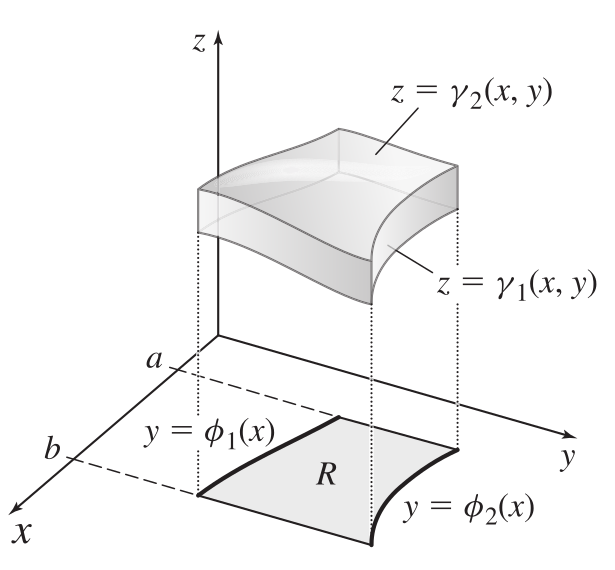
\includegraphics[width=0.5\linewidth]{images/lec-15-triple} 

}

\caption{Type I triple integral}\label{fig:unnamed-chunk-29}
\end{figure}

\begin{exercise}
\protect\hypertarget{exr:unlabeled-div-118}{}\label{exr:unlabeled-div-118}

Evaluate \(\displaystyle \iiint_D y~dV\) where \(D\) is the prism bounded by the planes \(x=0, x=2, y=0, z=0,\), and \(y+z=1\).

\end{exercise}

\begin{solution}

The prism can be described by the inequalities \(0\leq x\leq 2\), \(0\leq y \leq 1\), and \(0\leq z\leq 1-y\). We can set up and solve the following integral:

\begin{align*}
\iiint_D y~dV &= \int_0^2\int_0^1\int_0^{1-y}~dzdydx \\
&= \int_0^2 \int_0^1 1-y^2~dydx\\
&= \int_0^2 \frac{1}{6}~dx\\
&= \frac{1}{3}
\end{align*}

\end{solution}

\begin{exercise}
\protect\hypertarget{exr:unlabeled-div-120}{}\label{exr:unlabeled-div-120}

Evaluate \(\displaystyle \iiint_D \frac{z}{4-y} dV\) where \(D\) is the region lying in the first octant bounded by the cylinder \(y^2+z^2=4\) and the planes \(x+y=2\), \(x+2y=6\), \(z=0\), and \(y=0\).

\end{exercise}

\begin{solution}

Note that we can describe \(x\) in terms of \(y\) using the inequalities \(2-y\leq x\leq 6-2y\) and we can describe \(z\) using the inequalities \(0\leq z\leq \sqrt{4-y^2}\). The value of \(y\) is restricted to be between \(0\) (condition \(y=0\)) and \(2\) (condition \(\sqrt{4-y^2}\)).

Given that \(y\) is bounded by constants, we will integrate last with respect to \(y\); the other two conditions are interchangeable. However, things will be simpler if we integrate first with respect to \(x\) since the integrand is not a function of \(x\).

We have

\begin{align*}
\iiint_D \frac{z}{4-y} dV & = \int_0^2 \int_{0}^{\sqrt{4-y^2}}\int_{2-y}^{6-2y} \frac{z}{4-y}~dxdzdy \\
&= \int_0^2 \int_{0}^{\sqrt{4-y^2}} z~dz dy\\
&= \int_0^2 \frac{4-y^2}{2}~dy\\
&= \frac{8}{3}
\end{align*}

\end{solution}

\hypertarget{lec-16}{%
\chapter{Cylindrical Coordinates}\label{lec-16}}

Text References: Course notes pp.~66-74 \& Rogawski 15.3-15.6

\hypertarget{recap-14}{%
\section{Recap}\label{recap-14}}

Last time, we generalized our results and techniques for solving double integrals in order to solve triple integrals.

\begin{exercise}
\protect\hypertarget{exr:unlabeled-div-122}{}\label{exr:unlabeled-div-122}

Which of the following integrals is equal to \(\displaystyle \int_0^3 \int_0^2\int_0^y f(x,y,z)~dzdydx\)?

\begin{enumerate}
\def\labelenumi{\alph{enumi}.}
\tightlist
\item
  \(\displaystyle \int_0^2 \int_0^3\int_0^y f(x,y,z)~dzdxdy\)
\item
  \(\displaystyle \int_0^2 \int_0^3\int_0^y f(x,y,z)~dzdydx\)
\item
  \(\displaystyle \int_0^3 \int_0^2\int_0^y f(x,y,z)~dxdydz\)
\item
  \(\displaystyle \int_0^3 \int_0^2\int_0^z f(x,y,z)~dydzdx\)
\end{enumerate}

You can use this \href{https://www.geogebra.org/m/an5kuqrz}{interactive applet} to view the region in 3D.

\end{exercise}

\begin{solution}

The region can be described by the inequalities \(0\leq x\leq3\), \(0\leq y \leq 2\), and \(0\leq z\leq y\). Option a is simply swapping the constant bounds so it is equal to the initial integral.

\end{solution}

\hypertarget{learning-objectives-15}{%
\section{Learning Objectives}\label{learning-objectives-15}}

\begin{itemize}
\tightlist
\item
  Evaluate triple integrals by using an appropriate change to cylindrical coordinates.
\end{itemize}

\hypertarget{cylindrical-coordinates}{%
\section{Cylindrical Coordinates}\label{cylindrical-coordinates}}

So far, we've generalized most of our integration techniques from double to triple integrals. The last thing we'll cover on this topic are two key changes of variable: cylindrical coordinates and spherical coordinates.

\textbf{Cylindrical coordinates} are the 3D analogue to polar coordinates. In fact, the transformation is quite similar: \[x=\rho\cos(\phi), \quad y=\rho\sin(\phi), \quad\mbox{and}\quad z=z\]

Note that \(0\leq\phi < 2\pi\).

This \href{https://www.geogebra.org/m/uvsase6h}{interactive applet} might give you a geometric intuition for this coordinate system.

The Jacobian of this change of variables is \[\frac{\partial (x,y,z)}{\partial (\rho,\phi, z)}=\det \begin{bmatrix}x_{\rho}& x_{\phi}& x_{z} \\
y_{\rho}& y_{\phi}& y_{z} \\ z_{\rho}& z_{\phi}& z_{z} \end{bmatrix}=\det \begin{bmatrix}cos(\phi)& -\rho\sin(\phi) & 0 \\ \sin(\phi) & \rho\cos(\phi) & 0 \\ 0 & 0 & 1\end{bmatrix}=\rho\]

So, when changing from Cartesian to cylindrical coordinates, we can replace \(dzdydx\) with \(\rho~dzd\rho d\phi\), and this will almost always be the desired order of differentials.

\begin{exercise}
\protect\hypertarget{exr:unlabeled-div-124}{}\label{exr:unlabeled-div-124}

A wedge is cut from the cylinder \(x^2+y^2=4\) , by the planes \(z=0\) and \(z=3y\) , where \(y\) is assumed to be non-negative. Find the volume of the wedge.

\begin{figure}

{\centering 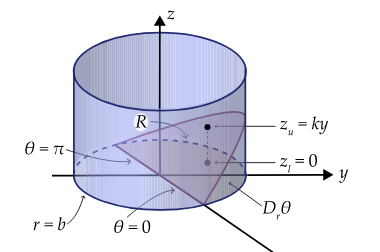
\includegraphics[width=0.75\linewidth]{images/lec-16-ex-1} 

}

\caption{Sketch of the wedge}\label{fig:unnamed-chunk-30}
\end{figure}

\end{exercise}

\begin{solution}

Converting the cylinder and the planes to cylindrical coordinates, we get \[x^2+y^2=4 \to \rho=2, \quad z=0 \to z=0, \quad z=3y\to z=3\rho\sin(\phi) \]

We can therefore describe the wedge using the following inequalities: \[0\leq \rho\leq 2, \quad 0\leq \phi\leq \pi,\quad \mbox{and}\quad 0\leq z \leq 3\rho\sin(\phi)\]

The last piece we need to recall is that the volume is given by \(\displaystyle V=\iiint_R 1~dV\).

Applying the change of variables, we get

\begin{align*}
V & =\iiint_R 1~dV\\
&= \int_0^{\pi}\int_0^2\int_0^{3\rho\sin (\phi)} \rho~dzd\rho d\phi\\
&= \int_0^{\pi}\int_0^2 3\rho^2\sin(\phi)~d\rho d\phi\\
&= \int_0^{\pi} 8\sin(\phi)~d\phi \\
&= 16
\end{align*}

\end{solution}

\hypertarget{lec-17}{%
\chapter{Spherical Coordinates}\label{lec-17}}

Text References: Course notes pp.~66-74 \& Rogawski 15.3-15.6

\hypertarget{recap-15}{%
\section{Recap}\label{recap-15}}

Last time, we discussed changing variables to cylindrical coordinates.

\begin{exercise}
\protect\hypertarget{exr:unlabeled-div-126}{}\label{exr:unlabeled-div-126}

Which of the following integrals is equal to \(\displaystyle \int_{-5}^5 \int_0^3\int_{-\sqrt{25-x^2}}^{\sqrt{25-x^2}} x~dydzdx\)?

\begin{enumerate}
\def\labelenumi{\alph{enumi}.}
\tightlist
\item
  \(\displaystyle \int_{0}^3 \int_0^3\int_{0}^{\pi} \rho^2\cos(\phi)~d\phi dzd\rho\)
\item
  \(\displaystyle \int_{0}^5 \int_0^3\int_{0}^{\pi} \rho^2\cos(\phi)~d\phi dzd\rho\)
\item
  \(\displaystyle \int_{0}^3 \int_0^5\int_{0}^{2\pi} \rho\cos(\phi)~d\phi dzd\rho\)
\item
  \(\displaystyle \int_{0}^5 \int_0^3\int_{0}^{2\pi} \rho^2\cos(\phi)~d\phi dzd\rho\)
\end{enumerate}

\end{exercise}

\begin{solution}

The region of integration is a cylinder of radius \(\rho=5\) and height \(z=3\). The integrand \(x~dydzdx\) becomes \(\rho\cos(\phi)\cdot \rho = \rho^2\cos(\phi)\). The corresponding integral is d.

\end{solution}

\hypertarget{learning-objectives-16}{%
\section{Learning Objectives}\label{learning-objectives-16}}

\begin{itemize}
\tightlist
\item
  Evaluate triple integrals by using an appropriate change to spherical coordinates.
\end{itemize}

\hypertarget{spherical-coordinates}{%
\section{Spherical Coordinates}\label{spherical-coordinates}}

\textbf{Spherical coordinates} are another way to generalize polar coordinates using the distance \(r\) from the origin and two angles. The angle \(\phi\) is defined in the same way as it is for cylindrical coordinates (i.e.~\(0\leq \phi < 2\pi\)). The angle \(\theta\) is the angle away from the positive \(z\)-axis (i.e.~\(0\leq \theta \leq \pi\)). The transformation is given by \[x=r\sin(\theta)\cos(\phi), \quad y=r\sin(\theta)\sin(\phi), \quad \mbox{and}\quad z= r\cos(\theta)\]

This \href{https://www.geogebra.org/m/kzfa7ybh}{interactive applet} might give you a geometric intuition for this coordinate system.

The Jacobian of this change of variables is \[\frac{\partial (x,y,z)}{\partial (r,\theta, \phi)}=\det \begin{bmatrix}x_{r}& x_{\theta}& x_{\phi} \\
y_{r}& y_{\theta}& y_{\phi} \\ z_{r}& z_{\theta}& z_{\phi} \end{bmatrix}=r^2\sin(\theta)\]

So, when changing from Cartesian to spherical coordinates, we can replace \(dV\) with \(r^2\sin(\theta)~drd\theta d\phi\).

\begin{exercise}
\protect\hypertarget{exr:unlabeled-div-128}{}\label{exr:unlabeled-div-128}

Evaluate \(\displaystyle \iiint_D \frac{1}{x^2+y^2+z^2}dV\) where \(D\) is the spherical shell between the spheres of radius \(3\) and radius \(5\) centred at the origin.

\end{exercise}

\begin{solution}

Note that a sphere of radius \(k\) can be described in spherical coordinates by \(0\leq r\leq k\), \(0\leq \theta \leq \pi\), and \(0\leq \phi < 2\pi\). Using this information helps us describe the region of integration as follows: \[3\leq r\leq 5, \quad \leq \theta \leq \pi, \quad \mbox{and} \quad 0\leq \phi < 2\pi\]

We can therefore describe the wedge using the following inequalities: \[0\leq \rho\leq 2, \quad 0\leq \phi\leq \pi,\quad \mbox{and}\quad 0\leq z \leq 3\rho\sin(\phi)\]

The integrand \(\dfrac{1}{x^2+y^2+z^2}\) becomes \(\dfrac{1}{r}\) in spherical coordinates. Putting everything together and applying the change of variables, we get

\begin{align*}
\iiint_D \frac{1}{x^2+y^2+z^2}dV & = \int_0^{2\pi}\int_0^{\pi}\int_3^5 \frac{1}{r^2}r^2\sin(\theta)~dr d\theta d\phi \\
& =  \int_0^{2\pi}\int_0^{\pi} 2\sin(\theta) d\theta d\phi \\
&=  \int_0^{2\pi} 4 d\phi\\
& = 8\pi
\end{align*}

\end{solution}

\hypertarget{spherical-vs-cylindrical-coordinates}{%
\section{Spherical vs Cylindrical Coordinates}\label{spherical-vs-cylindrical-coordinates}}

At this point, you might be wondering how to decide which coordinate system is best suited for a particular problem. Here is a general rule of thumb:

\begin{itemize}
\tightlist
\item
  Use cylindrical coordinates when there is symmetry about one of the three axes
\item
  Use spherical coordinates when there is symmetry about the origin
\end{itemize}

\hypertarget{lec-18}{%
\chapter{Newton's Method}\label{lec-18}}

Text References: Course notes pp.~75-100 \& Rogawski 4.8, 10.7

\hypertarget{recap-16}{%
\section{Recap}\label{recap-16}}

Last time, we discussed changing variables to spherical coordinates.

\begin{exercise}
\protect\hypertarget{exr:unlabeled-div-130}{}\label{exr:unlabeled-div-130}

Which of the following integrals give the volume of the unit sphere?

\begin{enumerate}
\def\labelenumi{\alph{enumi}.}
\tightlist
\item
  \(\displaystyle \int_{0}^{2\pi} \int_0^{2\pi}\int_{0}^{1} ~drd\phi d\theta\)
\item
  \(\displaystyle \int_{0}^{\pi} \int_0^{2\pi}\int_{0}^{1} ~drd\phi d\theta\)
\item
  \(\displaystyle \int_{0}^{\pi} \int_0^{2\pi}\int_{0}^{1} r^2\sin(\theta)~drd\phi d\theta\)
\item
  \(\displaystyle \int_{0}^{\pi} \int_0^{2\pi}\int_{0}^{1} r^2\sin(\theta)~drd\theta d\phi\)
\item
  \(\displaystyle \int_{0}^{\pi} \int_0^{2\pi}\int_{0}^{1} r~drd\theta d\phi\)
\end{enumerate}

\end{exercise}

\begin{solution}

The answer is c.~We must remember the Jacobian, which is equal to \(r^2\sin(\theta)\) and match the bounds: \(0\leq \theta \leq \pi\) and \(0\leq \phi \leq 2\pi\).

\end{solution}

\hypertarget{learning-objectives-17}{%
\section{Learning Objectives}\label{learning-objectives-17}}

\begin{itemize}
\tightlist
\item
  Use Newton's Method to find roots of polynomial equations.
\end{itemize}

\hypertarget{finding-roots-of-polynomials}{%
\section{Finding Roots of Polynomials}\label{finding-roots-of-polynomials}}

We're now going to switch back to working with functions of one variable. One type of problem that we'd like to solve is that of finding the roots of an equation, i.e.~solving \(f(x)=0\)interpola=1-x. solt . We're used to solving these problems algebraically, but this isn't always possible. Instead, we're going to develop numerical methods which can give us a good approximation of the roots.

As an example, consider the equation \(x^5=1-x\). If we want to find its solutions, we are solving \(x^5+x-1=0\); however there isn't a nice way of doing this algebraically.

Looking at the graph of this function, we notice that the root is located somewhere between \(x=0.5\) and \(x=1\).

\begin{figure}

{\centering 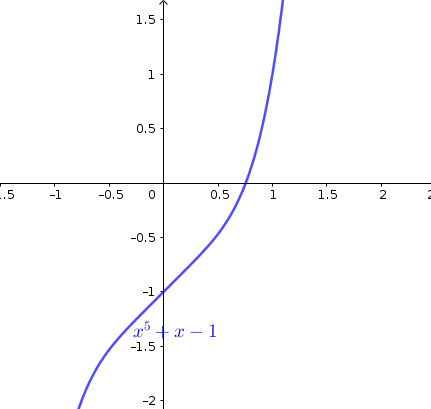
\includegraphics[width=0.5\linewidth]{images/lec-18-ex-1} 

}

\caption{Graph of $x^5+x-1$}\label{fig:unnamed-chunk-31}
\end{figure}

So, instead of finding exact solutions or roots to equations, we will have to make do with \emph{approximating} roots or solutions.

\hypertarget{newtons-method}{%
\section{Newton's Method}\label{newtons-method}}

\textbf{Newton's Method} is an iterative method for approximating roots of a function \(f(x)=0\), consisting of two main steps:

\begin{itemize}
\tightlist
\item
  Step 1: Choose an initial guess \(x_0\) that is close to the desired root, if possible.
\item
  Step 2: Generate successive approximations \(x_2, x_2\ldots\) where \(x_{n+1}=x_n-\dfrac{f(x)n}{f'(x_n)}\)
\end{itemize}

We can derive the formula in Step 2 by thinking about the linear approximation of \(f(x)\) at the point \(x_0\), which is given by \(L_{x_0}(x)=f(x_0)+f'(x_0)(x-x_0)\). This is the tangent line at \(x_0, f(x_0)\), which will cross the \(x\)-axis at the point \((x_1,0)\). Plugging this into the equation for the linear approximation and solving for \(x_1\), we get \[0=f(x_0)+f'(x_0)(x_1-x_0) \implies x_1=x_0+\dfrac{f(x_0)}{f'(x_0)}\] The same reasoning applies for \(x_2\) and so on.

In this \href{https://www.geogebra.org/m/ak4jpfjz}{interactive applet} we have an example of how Newton's Method works on the function \(f(x)=\frac{x^2}{2}+x+1-e^x\).

As with any numerical method, there are some caveats to keep in mind when using Newton's Method:

\begin{itemize}
\tightlist
\item
  The method will not converge if:

  \begin{itemize}
  \tightlist
  \item
    \(f'(x)\) does not exist or is not continuous at the root
  \item
    \(f'(x)=0\) at the root
  \item
    \(f''(x)\) is infinite at the root
  \end{itemize}
\item
  The method will converge rapidly \emph{as long as the initial guess for \(x_0\) is good enough}. A poor guess might result convergence to a different root or divergence. Coming up with a reasonable guess can be done by looking at the graph of the function.
\item
  In practice, it is usually safe to assume that if \(x_n\) and \(x_{n+1}\) agree to \(m\) decimal places, then the approximation is correct to these \(m\) places.
\end{itemize}

\begin{exercise}
\protect\hypertarget{exr:unlabeled-div-132}{}\label{exr:unlabeled-div-132}

Find a root of the function \(f(x)=x^5+x-1\), correct to five decimal places.

\end{exercise}

\begin{solution}

We have \(f'(x)=5x^4+1\). Looking at the graph of the function, we can set \(x_0=1\) as our initial guess for the root. Then,

\begin{align*}
x_1 &=x_0-\dfrac{f(x_0)}{f'(x_0)}=1-\dfrac{1}{6}=\frac{5}{6}\approx 0.83333 \\
x_2 &= x_1-\dfrac{f(x_1)}{f'(x_1)}\approx 0.76438 \\
x_3 &= x_2-\dfrac{f(x_2)}{f'(x_2)}\approx 0.75502 \\
x_4 &= x_3-\dfrac{f(x_3)}{f'(x_3)}\approx 0.75488 \\
x_5 &= x_4-\dfrac{f(x_4)}{f'(x_4)}\approx 0.75488 \\
\end{align*}

Note that at this point, the first five decimal places are no longer changing; this is the root, to five decimal places of accuracy.

\end{solution}

\begin{exercise}
\protect\hypertarget{exr:unlabeled-div-134}{}\label{exr:unlabeled-div-134}

Use three iterations of Newton's Method to find the smallest positive solution to \(\sin(3x)=\cos(x)\).

\begin{figure}

{\centering 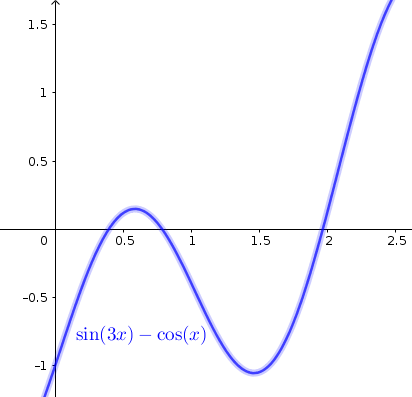
\includegraphics[width=0.5\linewidth]{images/lec-18-ex-2} 

}

\caption{Graph of $\sin(3x)-\cos(x)$}\label{fig:unnamed-chunk-32}
\end{figure}

\end{exercise}

\begin{solution}

A solution to \(\sin(3x)=\cos(x)\) is a root of \(f(x)=\sin(3x)-\cos(x)=0\). Looking at the graph of the function, we notice that the smallest root is located between \(x=0\) and \(x=0.5\). Let's use \(x_0=0.5\) as our initial guess.

We have \(f'(x)=3 \cos(3x)+\sin(x)\), which gives the formula \[x_{n+1}=x_n+\frac{\sin(3x_n)-\cos(x_n)}{ \cos(3x_n)+\sin(x_n)}\]
With \(x_0=0.5\) as the first guess, we have

\begin{align*}
x_1 \approx 0.326625\\
x_2 \approx 0.385204\\
x_3 \approx 0.392569
\end{align*}

\end{solution}

\hypertarget{lec-19}{%
\chapter{Interpolating Polynomials}\label{lec-19}}

Text References: Course notes pp.~75-100 \& Rogawski 4.8, 10.7

\hypertarget{recap-17}{%
\section{Recap}\label{recap-17}}

Last time, we learned about Newton's Method and how to apply it to find roots of a function.

\begin{exercise}
\protect\hypertarget{exr:unlabeled-div-136}{}\label{exr:unlabeled-div-136}

Consider the following questions:

\begin{enumerate}
\def\labelenumi{\alph{enumi}.}
\tightlist
\item
  How many iterations of Newton's Method are required to compute a root if \(f\) is a linear function?
\item
  What happens in Newton's Method if your initial guess happens to be a root of \(f\)?
\item
  What happens in Newton's Method if your initial guess happens to be a local min or max of \(f\)?
\end{enumerate}

\end{exercise}

\begin{solution}

We have:

\begin{enumerate}
\def\labelenumi{\alph{enumi}.}
\tightlist
\item
  Only one iteration is required; the function is equal to its linear approximation.
\item
  The iterates will all be equal to the initial guess \(x_0\).
\item
  The method will fail since \(f'(x)=0\) at local maxima and local minima.
\end{enumerate}

\end{solution}

\hypertarget{learning-objectives-18}{%
\section{Learning Objectives}\label{learning-objectives-18}}

\begin{itemize}
\tightlist
\item
  Use polynomial interpolation to find the polynomial of degree \(n\) which passes through a set of \(n+1\) points \((x_0,y_0), \ldots, (x_n,y_n)\).
\end{itemize}

\hypertarget{polynomial-interpolation}{%
\section{Polynomial Interpolation}\label{polynomial-interpolation}}

Suppose that we are given a set of \(n+1\) points \((x_0,y_0), \ldots, (x_n,y_n))\) and are asked to find a smooth curve which passes through all of them. The simplest curve that can achieve this is a polynomial of degree \(n\), that is, of the form \(y=a_0+a_x1+a_2x^2+\cdots+a_nx^n\).

This \href{https://www.geogebra.org/m/r4jkx4jh}{interactive applet} gives an idea of what we're trying to achieve:

The question we are now working on is how to find the equation of the polynomial passing through \((x_0,y_0), \ldots, (x_n,y_n))\).

\hypertarget{integer-nodes}{%
\subsection{Integer Nodes}\label{integer-nodes}}

Let's start by considering the simpler case where the values of \(x_0, y_0, x_1, y_1,\ldots\) are integers.

Suppose that we are looking for a degree \(3\) polynomial passing through the points \((0,y_0), (1, y_1), (2,y_2)\), and \((3,y_3)\).

We are looking for a cubic function \(y= a+bx+cx^2+dx^3\); plugging in our points gives

\begin{align*}
y_0 &= a \\
y_1 &= a+b+c+d\\
y_2 &= a+ 2b+4c+8d \\
y_3 &= a+3b+9c+27d
\end{align*}

Now, let's introduce some new notation. The \textbf{first finite differences} are \(\Delta y_n = y_{n+1}-y_n\)

\begin{exercise}
\protect\hypertarget{exr:unlabeled-div-138}{}\label{exr:unlabeled-div-138}

Calculate the first finite differences for the system above.

\end{exercise}

\begin{solution}

We have

\begin{align*}
\Delta y_0 &= y_1-y_0 = b+c+d \\
\Delta y_1 &= y_2-y_1 = b+3c+7d \\
\Delta y_2 &= y_3-y_1 = b+5c+19d \\
\end{align*}

\end{solution}

Notice that all of the \(a\)s have disappeared and we've eliminated one equation! Let's try to do the same trick with the \(b\)s.

The \textbf{second finite differences} are \(\Delta^2y_n = \Delta y_{n+1}-\Delta y_n\).

\begin{exercise}
\protect\hypertarget{exr:unlabeled-div-140}{}\label{exr:unlabeled-div-140}

Calculate the second finite differences for the system above.

\end{exercise}

\begin{solution}

\begin{align*}
\Delta^2 y_0 &= \Delta y_1 -\Delta y_0 = 2c+6d \\
\Delta^2 y_1 &= \Delta y_2 -\Delta y_1 = 2c+12d \\
\end{align*}

\end{solution}

Finally, the \textbf{third finite differences} are \(\Delta^3y_n = \Delta^2 y_{n+1}-\Delta^2 y_n\).

\begin{exercise}
\protect\hypertarget{exr:unlabeled-div-142}{}\label{exr:unlabeled-div-142}

Calculate the third finite differences for the system above.

\end{exercise}

\begin{solution}

We have

\begin{align*}
\Delta^2 y_0 &= \Delta^2 y_1 -\Delta^2 y_0 = 6d 
\end{align*}

\end{solution}

Now, we can rewrite our coefficients in terms of the finite differences with \(y_0\) as follows:

\begin{align*}
a &= y_0\\
b &= \Delta y_0 -\frac{1}{2} \Delta^2 y_0 + \frac{1}{3}\Delta^3 y_0\\
c &= \frac{1}{2}(\Delta^2 y_0 - \Delta^3 y_0)\\
d &= \frac{1}{6} \Delta^3 y_0
\end{align*}

Combining this with the equation of the polynomial, and with a bit of work, we get \[y=y_0+ \Delta y_0 x+ \frac{\Delta^2 y_0}{2}x(x-1)+ \frac{\Delta^3 y_0}{6}x(x-1)(x-2)\]

Generalizing to polynomials of degree \(n\) we get that the \(n\)th degree polynomial passing through the points\((0, y_0), (1,y_1),\ldots (n, y_n)\) is \[y= y_0 + \Delta y_0 x + \frac{\Delta^2 y_0}{2}x(x-1)+ \cdots + \frac{\Delta^n y_0}{n!}x(x-1)\cdots(x-n+1)\]

A useful way to calculate finite differences is by working with a triangular table. We write down the \(y\)-values and work out the finite differences from there. The table will look like this:

\begin{figure}

{\centering 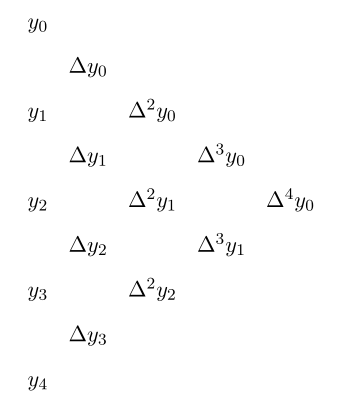
\includegraphics[width=0.4\linewidth]{images/lec-19-fd} 

}

\caption{Triangular table used to calculate finite differences}\label{fig:unnamed-chunk-33}
\end{figure}

\begin{exercise}
\protect\hypertarget{exr:unlabeled-div-144}{}\label{exr:unlabeled-div-144}

Find the \(4\)-th order polynomial which passes through the points \((0,5), (1, 7), (2, 19), (3,54)\), and \((4, 134)\)

\end{exercise}

\begin{solution}

We have \(y_0=5, y_1=7, y_2=19, y_3=54\), and \(y_4=134\).

Our first step is to find the finite differences.

The first finite differences are
\[\Delta y_0=y_1-y_0 = 2, \quad \Delta y_1 = y_2-y_1 = 12, \quad \Delta y_2 = y_3-y_2 = 35,\quad\mbox{and}\quad \Delta y_3 = y_4-y_3=80 \]

The second finite differences are
\[\Delta^2y_0 = \Delta y_1 -\Delta y_0 = 10, \quad \Delta^2y_1 = \Delta y_2 -\Delta y_1 = 23, \quad \Delta^2y_2 = \Delta y_3 -\Delta y_2=45\]

The third finite differences are
\[\Delta^3 y_0 = \Delta^2 y_1-\Delta^2 y_0=13, \quad \Delta^3 y_1 = \Delta^2 y_2- \Delta^2 y_1 = 22\]

The fourth finite difference is \(\Delta^4 y_0 = \Delta^3 y_1 -\Delta ^3 y_0 = 9\)

Plugging the relevant differences into the formula gives \[y=5+2x+5x(x-1)+\frac{13}{6}x(x-1)(x-2)+ \frac{3}{8}x(x-1)(x-2)(x-3)\]

\end{solution}

\hypertarget{non-integer-nodes}{%
\subsection{Non-Integer Nodes}\label{non-integer-nodes}}

Let's relax our previous assumptions a little by letting \(x_0, x_1, x_2,\ldots\) be any set of equidistant numbers, i.e.~\(x_n=x_0+nh\) for \(n=0,1,2,\ldots\) and \(h\) is the distance between each pair of points. Our polynomial interpolation formula generalizes to what's known as the \textbf{Newton Forward Difference Formula}:

Given \(n+1\) equidistant points \(x_0, x_1, \ldots, x_n\), the \(n\)th order polynomial passing through them is given by \[y= y_0 + \Delta y_0\frac{(x-x_0)}{h}\Delta y_0 + \frac{1}{2!}\Delta^2 y_0 \frac{(x-x_0)(x-x_1)}{h^2}+ \cdots + \frac{1}{n!}\Delta^n y_0 \frac{(x-x_0)(x-x_1)\cdots (x-x_{n-1})}{h^n}\]

\begin{exercise}
\protect\hypertarget{exr:unlabeled-div-146}{}\label{exr:unlabeled-div-146}

Estimate the value of \(f(1.35)\) if \(f(x)\) passes through the points \((1.2, 1),(1.3, 5),(1.4,12), (1.5, 20)\).

\end{exercise}

\begin{solution}

We have \(n=4\), \(h=0.1\), \(x_0=1.2, x_1=1.3, x_2=1.4, x_3=1.5\), \(y_0=1, y_1=5, y_2=12\), and \(y_3=20\).

The first finite differences are \[\Delta y_0 = 4, \quad \Delta y_1 =7, \quad \Delta y_2 = 8\]

The second finite differences are \[\Delta^2 y_0 = 3, \quad \Delta^2 y_1 =1\]

The third finite difference is \[\Delta^3 y_0 = -2\]

Plugging the relevant differences into the formula gives

\begin{align*}
y &=1+ 4\cdot\frac{x-1.2}{0.1}+ \frac{3}{2}\frac{(x-1.2)(x-1.3)}{0.1^2}-\frac{1}{12}\frac{(x-1.2)(x-1.3)(x-1.4)}{0.1^3}\\
&= 1+ 40(x-1.2)+150(x-1.2)(x-1.3)-\frac{1000}{3}(x-1.2)(x-1.3)(x-1.4)
\end{align*}

Finally, we input the value \(x=1.35\) to get \(f(1.35)\approx 8.25\)

\end{solution}

\hypertarget{lec-20}{%
\chapter{Taylor Polynomials}\label{lec-20}}

Text References: Course notes pp.~75-100 \& Rogawski 4.8, 10.7

\hypertarget{recap-18}{%
\section{Recap}\label{recap-18}}

Last time, we learned a method to fit a polynomial of degree \(n\) to a set of \(n+1\) points.

\hypertarget{learning-objectives-19}{%
\section{Learning Objectives}\label{learning-objectives-19}}

\begin{itemize}
\tightlist
\item
  Find the \(n\)th order Taylor polynomial for a given function.
\end{itemize}

\hypertarget{motivation}{%
\section{Motivation}\label{motivation}}

To motivate Taylor polynomials, let's think back to a few key ideas we've discussed so far.

The first idea is that of linear approximations. We've seen that the linear approximation of a function \(f(x)\) at \(x_0)\) is given by \(y=f(x_0)+\dfrac{\Delta y}{\Delta x}(x-x_0)\). Note that as we take the limit \(\Delta x \to 0\) of \(\dfrac{\Delta y}{\Delta x}\), we get the derivative of \(f\), so the linear approximation can be written as \(y=f(x_0)+f'(x_0)(x-x_0)\).

What if we want to approximate our function with polynomials instead? For simplicity, let's start by trying to approximate a function using a parabola. Here's where our second key idea of the Newton Forward Difference Formula comes in.

Suppose that we have a function at the equidistant points \(x_0\), \(x_1=x_0+\Delta x\), and \(x_2 = x_0 +2 \Delta x\). The corresponding \(y\) values will be \(y_0=f(x_0)\), \(y_1 = f(x_1)=f(x_0+\Delta x)\), and \(y_2=f(x_2)=f(x_0+2\Delta x)\). We can apply the Newton Forward Difference Formula to get the equation of the parabola that joins these three points: \[y=y_0+\frac{\Delta y_0}{\Delta x}(x-x_0)+ \frac{1}{2}\frac{\Delta^2 y_0}{(\Delta x)^2}(x-x_0)(x-x_1)\]

Now, let's take the limit as \(\Delta x \to 0\). We already know that \(\dfrac{\Delta y_0}{\Delta x}\to f'(x_0)\); you might guess (correctly!) that \(\dfrac{\Delta^2 y_0}{\Delta x^2}\to f''(x_0)\). Finally, we have that \(x_1\to x_0\). Putting everything together, we get a \emph{quadratic approximation} to \(f(x)\): \[y= f(x_0)+f'(x_0)(x-x_0)+\frac{1}{2}f''(x_0)(x-x_0)^2\]

The following \href{https://www.geogebra.org/m/csdwdaxd}{interactive applet} is designed to give you an intuition for what's going on both with the linear approximation and the quadratic approximation. Use the checkbox to display either the linear or quadratic approximation of the function. Use the slider to shorten the distance between the points \(x_0\), \(x_1\) (and \(x_2\) for the quadratic approximation). Notice what happens to the approximations as \(\Delta x \to 0\).

\hypertarget{taylor-polynomials}{%
\section{Taylor Polynomials}\label{taylor-polynomials}}

Now that we've got the flavour of things. we can extend this idea to a polynomial of degree \(n\). The \textbf{n-th order Taylor Polynomial centred at \(x_0\)} is \[P_{n, x_0}(x)= f(x_0)+f'(x_0)(x-x_0)+\frac{1}{2!}f''(x_0)(x-x_0)^2+\cdots+\frac{1}{n!}f^{(n)}(x_0)(x-x_0)^n\]

We can also write it more concisely using summation notation: \[P_{n, x_0}(x)= \sum_{k=0}^n \frac{f^{(k)}(x_0)}{k!}(x-x_0)^k\]

As you might expect, higher degree polynomial approximations typically give better approximations.

This \href{https://www.geogebra.org/m/m7knseej}{interactive applet} demonstrates how the Taylor polynomial can be used to approximate functions. Try a few functions out for yourself!

\begin{exercise}
\protect\hypertarget{exr:unlabeled-div-148}{}\label{exr:unlabeled-div-148}

Find the 3rd-order Taylor polynomial for \(f(x)=\sqrt{x+1}\) centred at \(3\).

\end{exercise}

\begin{solution}

We have \[f'(x)=\frac{1}{2}(x+1)^{-1/2}, \quad f''(x)= -\frac{1}{4}(x+1)^{-3/2}, \quad f'''(x)= \frac{3}{8}(x+1)^{-5/2}\]

Evaluating at \(x=3\), we get \[f'(3)=\frac{1}{4}, \quad f''(3) = -\frac{1}{32}, \quad f'''(3) = \frac{3}{256}\]

The Taylor polynomial is given by

\begin{align*}
P_{3,3}(x) &= 2+ \dfrac{1}{4}(x-3)+\frac{1}{2!}\frac{1}{32}(x-3)^2+ \frac{1}{6}\frac{3}{256}(x-3)^3\\
&= 2+ \frac{1}{4}(x-3)-\frac{1}{64}(x-3)^2+\frac{1}{512}(x-3)^3
\end{align*}

\end{solution}

\begin{exercise}
\protect\hypertarget{exr:unlabeled-div-150}{}\label{exr:unlabeled-div-150}

Find the 4th-order Taylor polynomial for \(f(x)=\dfrac{1}{1-x}\) centred at \(0\).

\end{exercise}

\begin{solution}

We have \[f'(x)=\frac{1}{(1-x)^2}, \quad f''(x) = \frac{2}{(1-x)^3}, \quad f'''(x)=\frac{6}{(1-x)^4}, \quad f^{(4)}(x) = \frac{24}{(1-x)^5}\]

and \[f'(0)=1, \quad f''(0)=2, \quad f'''(0)=6, \quad f^{(4)}(x)=24\]

then,

\begin{align*}
P_{4,0}(x) &= 1+1\cdot x + \frac{1}{2!}2x^2+\frac{1}{3!}6x^3+\frac{1}{4!}24x^4\\
&= 1+x+x^2+x^3+x^4
\end{align*}

\end{solution}

\hypertarget{lec-21}{%
\chapter{Taylor Polynomial Shortcuts}\label{lec-21}}

Text References: Course notes pp.~100-103 \& Rogawski 10.7

\hypertarget{recap-19}{%
\section{Recap}\label{recap-19}}

Last time, we learned about the Taylor polynomial of a function centred at a point.

\begin{exercise}
\protect\hypertarget{exr:unlabeled-div-152}{}\label{exr:unlabeled-div-152}

Find the 2nd-order Taylor polynomial for \(f(x)=e^x\) centred at \(0\).

\end{exercise}

\begin{solution}

We have \[f'(x)=f''(x)=e^x\]

and \[f'(0)=f''(0)=1\]

then,

\begin{align*}
P_{2,0}(x) &= f(0)+f'(0) x + \frac{1}{2!}f''(0)x^2\\
&= 1+x+\frac{1}{2}x^2
\end{align*}

\end{solution}

\hypertarget{learning-objectives-20}{%
\section{Learning Objectives}\label{learning-objectives-20}}

\begin{itemize}
\tightlist
\item
  Find the \(n\)th order Taylor polynomial for a given function using appropriate shortcuts.
\end{itemize}

\hypertarget{uniqueness-of-taylor-polynomials}{%
\section{Uniqueness of Taylor Polynomials}\label{uniqueness-of-taylor-polynomials}}

Now that we've defined \(n\)th order Taylor polynomials, for some function \(f(x)\) centred at \(x_0\), we might ask ourselves whether the Taylor polynomials are unique. Let's try to prove this.

Suppose that \(p(x)=a_0+a_1(x-x_0)+a_2(x-x_0)^2+\cdots +a_n(x-x_0)^n\) is a polynomial approximation of some function \(f(x)\) at point \(x_0\). We're going to try to figure out the values of the coefficients \(a_0, a_1,\ldots, a_n\).

At \(x_0\), we have \(p(x_0)=a_0\); this should be equal to \(f(x_0)\), which means that \(a_0=f(x_0)\).

Now, let's differentiate \(p(x)\) and evaluate at \(x_0\); this should be equal to \(f'(x_0)\). We have \[p'(x)=a_1+2a+2(x-x_0)+3a_3(x-x_0)^2+\cdots + n a_n(x-x_0)^{n-1}\]
at \(x=x_0\), we're left with \(p'(x_0)=a_1 = f'(x_0)\)

We can continue taking derivatives of \(p(x)\) and evaluating them at \(x=x_0\). As you might have guessed, we will get that \(a_n=\frac{1}{n!}f^{(n)}(x_0)\). So, indeed, the Taylor polynomial of a function centred at a point is unique!

Not only is the Taylor polynomial unique, but we now know that if we can find a polynomial which matches the values of \(f\) and its derivatives at a point, then that polynomial \emph{must} be the Taylor polynomial!

Let's state this more formally:

\begin{theorem}
\protect\hypertarget{thm:unlabeled-div-154}{}\label{thm:unlabeled-div-154}

Let \(p(x)=a_0+a_1(x-x_0)+\cdots +a_n(x-x_0)^n\). If \(p^{(k)}(x_0)=f^{(k)}(x_0)\) for all \(k=0, 1, 2,\ldots, n\), then \(p(x)=P_{n, x_0}(x)= \sum_{k=0}^n \frac{f^{(k)}(x_0)(x-x_0^k)}{k!}\)

\end{theorem}

\hypertarget{maclaurin-polynomials}{%
\section{Maclaurin polynomials}\label{maclaurin-polynomials}}

We give a special name to Taylor polynomials centred at zero:

\begin{definition}
\protect\hypertarget{def:unlabeled-div-155}{}\label{def:unlabeled-div-155}

A \textbf{Maclaurin polynomial} has the general form \(P_{n,0}(x)=\sum_{k=0}^n\frac{f^{(k)}(0)}{k!}x^k\)

\end{definition}

A consequence of the result that we've discussed is the following:

\begin{theorem}
\protect\hypertarget{thm:unlabeled-div-156}{}\label{thm:unlabeled-div-156}

If \(p(x)\) is the \(n\)th degree Maclaurin polynomial for \(f(x)\), then \(p(k x^m)\) is the (\(mn\))th degree Maclaurin polynomial for \(f(kx^m)\).

\end{theorem}

\begin{exercise}
\protect\hypertarget{exr:unlabeled-div-157}{}\label{exr:unlabeled-div-157}

Find the 6th-order Maclaurin polynomial for \(g(x)=e^{x^3}\) centred at \(0\).

\end{exercise}

\begin{solution}

We notice that \(g(x)=f(x^3)\) where \(f(x)=e^x\). Since \(p(x)=1+x+\frac{x}{2}\) is the second degree Maclaurin polynomial for \(f(x)\), the sixth degree Maclaurin polynomial for \(g(x)=f(x^3)\) is \[q(x)= 1+x^3+\frac{1}{2}(x^3)^2 = 1+ x^3+\frac{1}{2}x^6\]

\end{solution}

\hypertarget{other-shortcuts}{%
\section{Other Shortcuts}\label{other-shortcuts}}

Here are a few other ways to use Taylor polynomials. Suppose that \(p(x)\) is the \(n\)th order Taylor polynomial for \(f(x)\) centred at \(x_0\), that is, \[p(x_0)=f(x_0), \quad p'(x_0)=f'(x_0), \ldots, \quad p^{(n)}(x_0)=f^{(n)}(x_0)\]
then,

\begin{enumerate}
\def\labelenumi{\arabic{enumi}.}
\tightlist
\item
  \(f'(x)\) can be approximated by \(p'(x)=P_{n-1,x_0}(x)\)
\item
  \(\displaystyle \int f(x)dx\) can be approximated by \(\displaystyle \int p(x)dx = P_{n+1,x_0}(x)\) (but be careful with \(C\)!)
\end{enumerate}

\hypertarget{lec-22}{%
\chapter{Taylor's Remainder Theorem}\label{lec-22}}

Text References: Course notes pp.~103-106 \& Rogawski 10.7

\hypertarget{recap-20}{%
\section{Recap}\label{recap-20}}

Last time, we learned some result to help us calculate Taylor polynomials more easily.

\begin{exercise}
\protect\hypertarget{exr:unlabeled-div-159}{}\label{exr:unlabeled-div-159}

Find the 10th-order Maclaurin polynomial for \(h(x)=\sin(3x^2)\) given that the fifth-order Maclaurin polynomial for \(f(x)=\sin(x)\) is \(P_{5,0}(x)=x-\frac{x^3}{3!}+\frac{x^5}{5!}\).

\end{exercise}

\begin{solution}

We notice that \(h(x)=f(3x^2)\). Since Since \(p(x)=x-\frac{x^3}{3!}+\frac{x^5}{5!}\) is the second degree Maclaurin polynomial for \(f(x)\), the tenth degree Maclaurin polynomial for \(h(x)=f(3x^2)\) is \[r(x)=3x^2-\frac{(3x^2)^3}{3!}+\frac{(3x^2)^5}{5!}= 3x^2-\frac{9}{2}x^6+\frac{81}{40}x^{10}\]

\end{solution}

\hypertarget{learning-objectives-21}{%
\section{Learning Objectives}\label{learning-objectives-21}}

\begin{itemize}
\tightlist
\item
  N/A
\end{itemize}

\hypertarget{taylors-remainder-theorem}{%
\section{Taylor's Remainder Theorem}\label{taylors-remainder-theorem}}

Now that we've got a good handle on computing Taylor polynomials, we might start to wonder: how accurate is this approximation. In other words. how closely does \(P_{n, x_0}(x)=\sum_{k=0}^n \frac{f^{}(k)}(x_0)(x-x_0)^k{k!}\) approximate \(f(x)\). Yet another way to formulate this is how big is the error \(|f(x)-P_{n, x_0}(x)|\)?

We are going to work towards answering this question in the next few lessons. Today, we will focus on an intermediate result called \textbf{Taylor's Remainder Theorem}.

Our more immediate goal is to try to understand the error term \(|f(x)-P_{n, x_0}(x)|\). Let's start by considering the simplest case where \(P_{n, x_0}\) is a constant, that is, the zeroth order Taylor polynomial. We have \[f(x)-P_{0,x_0}(x)=f(x)-f(x_0)\]
By the Fundamental Theorem of Calculus, we get \[f(x)-P_{0,x_0}(x)=\int_{x_0}^x f'(t)dt\]
This expression might seem more complicated than what we started with, but it will pay off in the long run, so let's stick with it.

Now, let's consider the case of the first order Taylor polynomial. That is, let's consider the error in a linear approximation of \(f(x)\). We have \[f(x)-P_{0,x_0}(x)=f(x)-f(x_0)=f(x)- [f(x_0)+f'(x_0)(x-x_0)]\]
We see that the term \(f(x)-f(x_0)\) is making an appearance, so we can use the same integration trick as before: \[f(x)-P_{1,x_0}(x)=\int_{x_0}^x f'(t)dt-f'(x_0)(x-x_0)\]

We can further simplify this expression using integration by parts with \(u=f'(t)\) and \(v=t\) to get \[ f(x)-P_{1,x_0}(x)=\left[ t f'(t)\right |_{x_0}^x-\int_{x_0}^x tf''(t)dt - f'(x_0)(x-x_0)\]

With a bit more algebra magic, we end up with \[f(x)-P_{1,x_0}(x)=\int_{x_0}^x (x-t)f''(t)dt\]
The key point here is that we've come up with a more tidy expression for the error term.

Repeating this process for the second order Taylor polynomial, we find \[f(x)-P_{2,x_0}(x)=\int_{x_0}^x \frac{(x-t)^2f'''(t)}{2}dt\]

At this point, we have a general idea of how the pattern works, so let's write it out formally.

\begin{theorem}
\protect\hypertarget{thm:unlabeled-div-161}{}\label{thm:unlabeled-div-161}

If \(f(x)\) has \(n+1\) derivatives at \(x_0\), then \[f(x)=\sum_{k=0}^n \frac{f^{(k)}(x_0)(x-x_0)^k}{k!}+R_n(x)\] where \[R_n(x)=\int_{x_0}^x\frac{(x-t)^n}{n!}f^{(n+1)}(t)dt\]

\end{theorem}

We call \(R_n(x)\) the \textbf{remainder} or the \textbf{error} in the approximation. Calculating this remainder isn't actually possible. What we're going to aim for instead is finding an \emph{upper bound} on the error, so we can know how far off our approximation is in the worst-case scenario.

\hypertarget{lec-23}{%
\chapter{Taylor's Inequality}\label{lec-23}}

Text References: Course notes pp.~107-110 \& Rogawski 10.7

\hypertarget{recap-21}{%
\section{Recap}\label{recap-21}}

Last time, we learned about Taylor's Remainder Theorem:

\begin{theorem}
\protect\hypertarget{thm:unlabeled-div-162}{}\label{thm:unlabeled-div-162}

If \(f(x)\) has \(n+1\) derivatives at \(x_0\), then \[f(x)=\sum_{k=0}^n \frac{f^{(k)}(x_0)(x-x_0)^k}{k!}+R_n(x)\] where \[R_n(x)=\int_{x_0}^x\frac{(x-t)^n}{n!}f^{(n+1)}(t)dt\]

\end{theorem}

\hypertarget{learning-objectives-22}{%
\section{Learning Objectives}\label{learning-objectives-22}}

\begin{itemize}
\tightlist
\item
  Compute an upper bound on the error in an \(n\)th order Taylor polynomial.
\end{itemize}

\hypertarget{taylors-inequality}{%
\section{Taylor's Inequality}\label{taylors-inequality}}

Remember that we're still working towards the goal of determining how accurate our Taylor polynomial approximations are. Last time, we were able to derive a relatively tidy expression for the remainder or error of a Taylor polynomial. Today, we're going to work on determining an upper bound for the error. In order to do this, we will rely on a generalization of the triangle inequality.

The triangle inequality you might be familiar with is \(|a+b|\leq |a|+|b|\). We can generalize it to an arbitrary number of sums to get \(\displaystyle \left | \sum_{i=1}n a_i \right | \leq \sum_{i=1}^n |a_i|\). Generalizing a bit more to Riemann sums gives \[\left |\int_a^b f(x)fx \right |\leq \int_a^b |f(x)|dx \quad \mbox{(assuming $a<b$)}\]

Going back to our expression for the error and applying the generalized triangle inequality, the magnitude of the error is:

\begin{align*}
|R_n(x)|&= \left | \int_{x_0}^x\frac{(x-t)^n}{n!}f^{(n+1)}(t)dt\right |\\
& \leq \int_{x_0}^x\frac{|x-t|^n}{n!}|f^{(n+1)}(t)|dt \quad \mbox{by the triangle inequality}\\
&= \leq \int_{x_0}^x\frac{|x-t|^n}{n!}Kdt  \quad \mbox{for a constant $K$ such that $|f^{(n+1)}(t)|\leq K$} \\
&= -K \left. \frac{|x-t|^{n+1}}{(n+1)!}\right |_{x_0}^x \\
&= K \frac{|x-x_0|^{n+1}}{(n+1)!}
\end{align*}

We can now state the general result:

\begin{theorem}
\protect\hypertarget{thm:unlabeled-div-163}{}\label{thm:unlabeled-div-163}

The error in using an \(n\)th order Taylor polynomial \(P_{n, x_0}(x)\) as an approximatino to \(f(x)\) satisfies the inequality \[|R_n(x)|\leq  K \frac{|x-x_0|^{n+1}}{(n+1)!} \] where \(f^{(n+1)}(t)|\leq K\) for all values of \(z\) between \(x_0\) and \(x\).

\end{theorem}

You might be wondering about this constant \(K\) and how to find it. In practice, we will know that the function \(f(x)\) is and we will be able to calculate the relevant derivative and bound it. There are a few tricks you can use:

\begin{itemize}
\tightlist
\item
  If the function is monotonic (i.e.~non-increasing or non-decreasing) on the interval \([x_0,x]\), then its maximum on the interval is found by evaluating the function at the endpoints.
\item
  If the function is not monotonic on the interval \([x_0,x]\) but can be written as products of monotonic functions, we can find the maximum for each factor and multiply them together.
\item
  If the function is not monotonic on the interval \([x_0,x]\) but can be written as a sum, we can use the triangle inequality to find a monotonic function that bounds it.
\item
  If the function is not monotonic on the interval \([x_0,x]\) we can find its maximum on that interval using our usual maximization techniques.
\end{itemize}

\begin{exercise}
\protect\hypertarget{exr:unlabeled-div-164}{}\label{exr:unlabeled-div-164}

Let \(f(x)=\cos(x)\) and suppose that \(P_{6,0}(x)=1- \frac{x^2}{2!}+\frac{x^4}{4!}-\frac{x^6}{6!}\) (You should check this for yourself!)

\begin{enumerate}
\def\labelenumi{\alph{enumi}.}
\tightlist
\item
  Use \(P_{6,0}(x)\) to approximate \(\cos(2)\).
\item
  Find an upper bound on the error term from part a.
\item
  For what values of \(n\) does \(P_{n,0}(2)\) approximate \(\cos(2)\) correct to \(4\) decimal places?
\end{enumerate}

\end{exercise}

\begin{solution}

We are given that \(P_{6,0}(x)=1- \frac{x^2}{2!}+\frac{x^4}{4!}-\frac{x^6}{6!}\).

\begin{enumerate}
\def\labelenumi{\alph{enumi}.}
\tightlist
\item
  Our estimate for \(\cos(2)\) is \[P_{6,0}(2)=1- \frac{2^2}{2!}+\frac{2^4}{4!}-\frac{2^6}{6!}=-\frac{19}{45}\approx -0.422\]
\item
  We will use Taylor's Inequality to find an upper bound on the error term. Note that \(\sin(x)\) is monotonic on \([0,2]\). We have \[f^{(7)}(x)=|\sin(x)|\leq 1\quad\mbox{for all $x\in[0,2]$}\] so we can set \(K=1\). Applying Taylor's Inequality, \[|R_6(2)|\leq K \frac{|2-0|^{6+1}}{(6+1)!}=\frac{1\cdot 2^7}{7!}=\frac{8}{315}\]
  This means that the error is bounded above by \(\frac{8}{315}\approx 0.0254\). In other words, the value of \(\cos(2)\) lies in the interval \([-\frac{19}{45}-\frac{8}{315}, -\frac{19}{45}+\frac{8}{315}]\approx [-0.448, -0.396]\)
\item
  The approximation \(P_{n,0}(2)\) being correct to \(4\) decimal places means that the error term is less than \(10^{-4}\). That is, \[R_{n}(2)\leq K \frac{(x-x_0)^{n+1}}{(n+1)!} < 10^{-4}\]
\end{enumerate}

We have \[R_{n}(2)\leq K \frac{|x-x_0|^{n+1}}{(n+1)!} = \frac{1\cdot |2-0|^{n+1}}{(n+1)!} = \frac{2^{n+1}}{(n+1)!}\]
At this point, we're going to have to do a bit of trial and error to find a value of \(n\) that works. Remember, we're looking for a value of \(n\) that makes the remainder less than \(10^{-4}\). Our previous work found that at \(n=6\), the error is approximately \(0.0254\), which is greater than \(10^{-4}\). Let's start from \(n=7\) and go from there.

\begin{itemize}
\tightlist
\item
  When \(n=7\), \(|R_7(x)|\leq \frac{2^8}{8!}\approx 0.00635\)
\item
  When \(n=8\), \(|R_8(x)|\leq \frac{2^9}{9!}\approx 0.00142\)
\item
  When \(n=9\), \(|R_9(x)|\leq \frac{2^{10}}{10!}\approx 0.00029\)
\item
  When \(n=10\), \(|R_{10}(x)|\leq \frac{2^{11}}{11!}\approx 0.00006 < 10^{-4}\)
\end{itemize}

Therefore \(P_{n,0}(2)\) approximates \(\cos(2)\) correct to \(4\) decimal places for values of \(n\) greater than or equal to \(10\).

Use this \href{https://www.geogebra.org/m/heswekn6}{interactive applet} to observe what's happening. The applet shows the function \(f(x)=\cos(x)\) along with the Taylor polynomial \(P_{n,0}(x)\). Use the slider to increase the value of \(n\) and observe how the magnitude of the remainder changes for \(x=2\). Note that the only two decimals can be displayed.

\end{solution}

\hypertarget{lec-24}{%
\chapter{Approximation of Integrals using Taylor Polynomials}\label{lec-24}}

Text References: Course notes pp.~111-114 \& Rogawski 10.7

\hypertarget{recap-22}{%
\section{Recap}\label{recap-22}}

Last time, we found a way to estimate the error bound of a Taylor polynomial.

\begin{exercise}
\protect\hypertarget{exr:unlabeled-div-166}{}\label{exr:unlabeled-div-166}

Find the error bound for the third order Taylor polynomial of \(f(x)=\ln(x)\) for centred at \(1\) and evaluated at \(x=1.2\).

\end{exercise}

\begin{solution}

First, we need to find a value of \(K\) such that \(|f^{(4)}(x)|\leq K\) for values of \(x\) between \(1\) and \(1.2\). We have \(f^{(4)}(x)=-6x^{-4}\) and so \(|f^{(4)}(x)|\) is decreasing on the interval \([1, 1.2]\). The maximum value on that interval is at \(x=1\), and so \(|f^{(4)}(x)|\leq f^{(4)}(1)=6\). We therefore set \(K\).

Applying Taylor's Inequality, we have \(\displaystyle |R_3(1.2)|\leq 6 \frac{|1.2-1|^4}{4!}\approx 0.0004\).

\end{solution}

\hypertarget{learning-objectives-23}{%
\section{Learning Objectives}\label{learning-objectives-23}}

\begin{itemize}
\tightlist
\item
  Use Taylor polynomials to approximate integrals.
\end{itemize}

\hypertarget{motivation-1}{%
\section{Motivation}\label{motivation-1}}

Now that we've developed a nice and robust theory of Taylor polynomials, it's time to put it to use. One particularly useful application is in approximating integrals for which there is no tidy antiderivative.

Let's work with a motivating example. Suppose that we want to estimate \(\displaystyle \int_0^1 e^{x^2}dx\). Our approach will be to replace \(e^{x^2}\) with a function that is close to \(e^{x^2}\) but is much easier to integrate. The Taylor polynomial of \(e^{x^2}\) is an excellent candidate: we know that it gives a good approximation of the function and polynomials are much easier to integrate.

\hypertarget{approximating-integrals-using-polynomials}{%
\section{Approximating Integrals using Polynomials}\label{approximating-integrals-using-polynomials}}

Let's take the second order Maclaurin polynomial of \(e^x\) and use it to find the second order Maclaurin polynomial of \(e^{x^2}\). We have \(P_{0,2}(x)=1+x+\frac{x^2}{2!}+R_2(x)\) and so \(P_{0,2}(x^2)=1+x^2+\frac{x^4}{2!}+R_2(x^2)\)

Now, we have to deal with those remainders--simply throwing them away with throw off the accuracy of our approximation.

Recall that \(\displaystyle |R_2(x)|\leq \frac{K|x-0|^3}{3!}\). We are working on the interval \([0,1]\) and so the third derivative of \(e^x\) is bounded above by \(e\). We can therefore set \(K=e\) to get \(\displaystyle |R_2(x)|\leq \frac{e|x|^3}{3!}\leq \frac{3|x|^3}{3!} = \frac{|x|^3}{2}\). Note that here, we rounded \(e\) up to \(3\) to get some nice cancellations.

Given that \(\displaystyle |R_2(x)|\leq\frac{|x|^3}{2}\) this means that \(\displaystyle |R_2(x^2)|\leq\frac{|x^2|^3}{2}=\frac{x^6}{2}\). That is, \[1+x^2+\frac{x^4}{2}-\frac{x^6}{2}\leq e^{x^2}\leq 1+x^2+\frac{x^4}{2}+\frac{x^6}{2}\]

Now that we have all of the pieces in place, we can get back to the integral:

\begin{align*}
 \int_0^1 e^{x^2}dx & \leq \int_0^1 1+x^2+\frac{x^4}{2!}+R_2(x^2) dx \\
&= \int_0^1 1+x^2+\frac{x^4}{2!}+\frac{x^6}{2} dx\\
&= \frac{158}{105} \approx 1.505\\
\end{align*}

Similarly, \[\int_0^1 1+x^2+\frac{x^4}{2}-\frac{x^6}{2}dx \leq \int_0^1 e^{x^2}dx \implies \frac{143}{105}\approx 1.361 \leq \int_0^1 e^{x^2}dx\]

We can therefore conclude that \[1.361 \leq \int_0^1 e^{x^2}dx \leq 1.505\]

\begin{exercise}
\protect\hypertarget{exr:unlabeled-div-168}{}\label{exr:unlabeled-div-168}

Estimate \(\displaystyle \int_0^{2/3}x\sin(x^3)dx\) using the tenth degree Maclaurin polynomial for \(x\sin(x^3)\). You may use the fact that \(P_{3,0}(x)=x-\frac{x^3}{3}+R_3(x)\) for \(f(x)=\sin(x)\).

\end{exercise}

\begin{solution}

We know that \(f(x)=x-\frac{x^3}{3}+R_3(x)\) and therefore for \(g(x)=x\cdot sin(x^3)\) we have \(g(x)=x\cdot f(x^3)=x\cdot \left (x^3-\frac{x^9}{6}+R_3(x^3)\right) = x^4-\frac{x^{10}}{6}+xR_3(x^3)\)

Now, let's work on the remainder. On the interval \(x\in [0, 2/3]\), we have \(x^3 \in [0, 8/27]\) \(|\sin(x)^{(4)}|=|\sin(x)|\leq 8/27\leq 1\). And so \[|R_3(x)|\leq \frac{1\cdot |x-0|^4}{4!}=\frac{x^4}{4!}\]

From here, we can find \[|xR_3(x^3)| \leq x\cdot \frac{(x^4)^3}{4!} = \frac{|x|^{13}}{48}\] since we are on an interval with \(x >0\), we can drop the absolute values on the numerator to get \(\displaystyle |xR_3(x^3)| \leq \frac{x^{13}}{48}\)

Putting everything together, we have

\begin{align*}
\int_0^{2/3}x\sin(x^3)dx &= \int_0^{2/3} x^4-\frac{x^{10}}{6}+xR_3(x^3) dx \\
&= \int_0^{2/3} x^4-\frac{x^{10}}{6}+\frac{x^{13}}{48}\\
& \approx 0.02616228 + 0.0000051\\
&= 0.02616738
\end{align*}

\end{solution}

\hypertarget{lec-25}{%
\chapter{Infinite Series}\label{lec-25}}

Text References: Course notes pp.~114-129 \& Rogawski 10.2-10.3

\hypertarget{recap-23}{%
\section{Recap}\label{recap-23}}

Last time, we wrapped up our study of Taylor polynomials and used them to compute integrals.

\hypertarget{learning-objectives-24}{%
\section{Learning Objectives}\label{learning-objectives-24}}

\begin{itemize}
\tightlist
\item
  State the Taylor series of a few well-known functions.
\item
  Identify sequences, sequences of partial sums, and series.
\end{itemize}

\hypertarget{taylor-series}{%
\section{Taylor Series}\label{taylor-series}}

We're going to extend the Taylor polynomial to the \textbf{Taylor series} of a function \(f(x)\). The Taylor series will include the terms of \emph{all} orders in the Taylor polynomial:

\begin{definition}
\protect\hypertarget{def:unlabeled-div-170}{}\label{def:unlabeled-div-170}

If \(f\) is infinitely differentiable at \(x_0\), then the \textbf{Taylor series} for \(f(x)\) centred at \(x_0\) is \[T(x)=f(x_0)+f'(x_0)(x-x_0)+\frac{f''(x_0)}{2!}(x-x_0)^2+\cdots  = \sum_{n=0}^{\infty}\frac{f^{(n)}(x_0)}{n!}(x-x_0)^n\]

\end{definition}

Let's take a look at two functions, \(f(x)=\sin(x)\) and \(g(x)=\frac{1}{1+x}\). The \href{https://www.geogebra.org/m/z2awkcej}{interactive applet} displays \(f(x)\) and \(g(x)\) along with their respective Taylor polynomials. Use the checkboxes to display either \(f(x)\) or \(g(x)\). Using the slider to increase the order of the Taylor polynomials, observe how well the Taylor polynomial approximates the value at \(x=2\).

It seems like the Taylor polynomial gives a better and better approximation of \(f(2)\), but the same can't be said for \(g(2)\). A natural question to ask is whether the Taylor series of a function is actually \emph{equal} to the function. We've seen a few examples (such as \(f(x)=\sin(x)\) where taking higher and higher order Taylor polynomials of a function results in better and better approximations. In these cases, we might expect that as \(n\to\infty\) the Taylor polynomial converges to the function.

In order to answer this question, we're going to revisit Taylor's Inequality. We have that \[f(x)=\sum_{k=0}^n\frac{f^{(k)}(x_0)}{k!}(x-x_0)^k+R_n(x)\] where \(|R_n(x)|\leq K \dfrac{|x-x_0|^{n+1}}{(n+1)!}\) with \(|f^{(n+1)}(z)|\leq K\) for all values of \(z\) between \(x\) and \(x_0\). Whether or not the Taylor series is equal to the function depends on what happens as we take the limit \(n\to\infty\). We have \[f(x)=^{?}\lim_{n\to\infty}\left [\sum_{k=0}^n\frac{f^{(k)}(x_0)}{k!}(x-x_0)^k+R_n(x) \right] =^? \lim_{n\to\infty}\sum_{k=0}^n\frac{f^{(k)}(x_0)}{k!}(x-x_0)^k + \lim_{n\to \infty}R_n(x)\]
We will have an equality of \(f(x)\) and its Taylor series if \(\displaystyle \lim_{n\to \infty}R_n(x)=0\); otherwise, we can still calculate the Taylor series of the function, but it won't be equal to \(f(x)\).

A warning about notation: when we write \(f(x)=\sum_{k=0}^\infty\frac{f^{(k)}(x_0)}{k!}(x-x_0)^k\), we really mean that \(f(x)=\lim_{n\to\infty}\sum_{k=0}^n\frac{f^{(k)}(x_0)}{k!}(x-x_0)^k\) for all \(x\).

Here are a few Taylor series you should know:

\begin{itemize}
\tightlist
\item
  \(\sin(x)=\sum_{n=0}^\infty (-1)^n \frac{x^{2n+1}}{(2n+1)!}=x-\frac{x^3}{3!}+\frac{x^5}{5!}-\frac{x^7}{7!}+\cdots\)
\item
  \(\cos(x)=\sum_{n=0}^\infty (-1)^n \frac{x^{2n}}{(2n)!}=1-\frac{x^2}{2!}+\frac{x^4}{4!}-\frac{x^6}{6!}+\cdots\)
\item
  \(e^x = 1+ x+ \frac{x^2}{2!}+\frac{x^3}{3!}+\cdots\)
\end{itemize}

The question of whether or not the remainder of a Taylor series goes to zero requires a few more tools that we're going to work on developing.

\hypertarget{infinite-series}{%
\section{Infinite Series}\label{infinite-series}}

We're going to leave Taylor series aside for the moment and focus on sequences and series.

Let's start with \textbf{sequences}, denoted by \(\{a_k\}\), which are ordered lists of numbers with elements indexed by the natural numbers.

From a sequence, we can build the \textbf{sequence of partial sums}, denoted by \(\{s_n\}\) and defined as

\begin{align*}
s_0 &= a_0 \\
s_1 &= a_0 + a_1 \\
s_2 &= a_0 + a_1 + a_2 \\
& \vdots \\
s_n &= a_0 + a_1 + a_2 + \cdots + a_n
\end{align*}

\begin{exercise}
\protect\hypertarget{exr:unlabeled-div-171}{}\label{exr:unlabeled-div-171}

Consider the sequence \(a_k=\dfrac{1}{2^k}\).

\begin{enumerate}
\def\labelenumi{\alph{enumi}.}
\tightlist
\item
  List the terms \(a_0, \ldots, a_3\) of the sequence.
\item
  Give the partial \(s_0, \ldots, s_3\) sums of the sequence.
\end{enumerate}

\end{exercise}

\begin{solution}

We have \(a_k=\dfrac{1}{2^k}\)

\begin{enumerate}
\def\labelenumi{\alph{enumi}.}
\tightlist
\item
  \(a_0= \dfrac{1}{2^0}=1, \quad a_1=\dfrac{1}{2^1}=\dfrac{1}{2}, \quad a_2=\dfrac{1}{2^2}=\dfrac{1}{4}, \quad a_3=\dfrac{1}{2^3}=\dfrac{1}{8}\)
\item
  We have
  \begin{align*}
  s_0 &= a_0=1 \\
  s_1 &= a_0+a_1=\dfrac{3}{2}=1.5\\
  s_2 &= a_0 + a_1 + a_2 = 1+\dfrac{1}{2}+\dfrac{1}{4} =\dfrac{7}{4} =1.75\\
  s_3 &= a_0 + a_1 + a_2 +a_3 = 1+\dfrac{1}{2}+\dfrac{1}{4} +\dfrac{1}{8} =\dfrac{15}{8} = 1.875 
  \end{align*}
\end{enumerate}

\end{solution}

Now, let's define \textbf{infinite series}:

\begin{definition}
\protect\hypertarget{def:unlabeled-div-173}{}\label{def:unlabeled-div-173}

An \textbf{infinite series} (or a \textbf{series}) of constant \(a_k\) is defined as a limit of finite series: \[\sum_{k=0}^\infty a_k =\lim_{n\to \infty}\sum_{k=0}^na_k\]

\end{definition}

We say that the series \(\sum_{k=0}^\infty a_k\) \textbf{converges} if the sequence \(\{s_n\}\) converges to some value \(s\), i.e.~if \(\displaystyle \lim_{n\to\infty}s_n=s\). Otherwise, we say that the series \textbf{diverges}.

Although is common to start the indexing for sequences and series at \(k=0\), we can start the index at any integer. If we happen to meet a series which doesn't start at \(k=0\), we can always re-index it using the following trick: \(\displaystyle \sum_{k=q}^\infty a_k = \sum_{k=0}^\infty a_{k+q}\). For questions of convergence of a series, it's common to omit the index value entirely and just write \(\displaystyle \sum a_k\).

Let's take a look at our exercise again and write out a few more of the partial sums:

\begin{align*}
s_0 & = 1\\
s_1 & = 1.5\\
s_2 & = 1.75\\
s_3 & = 1.875\\
s_4 & = 1.9375\\
s_5 & = 1.96875\\
s_6 & = 1.984375\\
\end{align*}

The series certainly appears to be converging to \(2\), but we don't have the tools to prove this yet. Soon, we will come up with several tests to determine whether a given series converges or diverges.

\hypertarget{lec-26}{%
\chapter{Convergence Tests Part 1}\label{lec-26}}

Text References: Course notes pp.~114-129 \& Rogawski 10.2-10.3

\hypertarget{recap-24}{%
\section{Recap}\label{recap-24}}

Last time, we discussed sequences, sequences of partial sums, and series. We also started a discussion around convergence and divergence of infinite series.

\begin{exercise}
\protect\hypertarget{exr:unlabeled-div-174}{}\label{exr:unlabeled-div-174}

Consider the sequence \(\{a_k\}=3x^k\).

\begin{enumerate}
\def\labelenumi{\alph{enumi}.}
\tightlist
\item
  List \(a_0,\ldots, a_3\).
\item
  Calculate \(s_0,\ldots, s_3\).
\end{enumerate}

\end{exercise}

\begin{solution}

For \(\{a_k\}=3x^k\), we have

\begin{enumerate}
\def\labelenumi{\alph{enumi}.}
\tightlist
\item
  \(a_0=3x^0=3, \quad a_1 =3x^1=3x, \quad a_2=3x^2, \quad a_3=3x^3\)
\item
  \begin{align*}
  s_0 &= 3 \\
  s_1 &= 3+3x \\
  s_2 &= 3+3x +3x^2\\
  s_3 &= 3+3x +3x^2 +3x^3
  \end{align*}
\end{enumerate}

\end{solution}

\hypertarget{learning-objectives-25}{%
\section{Learning Objectives}\label{learning-objectives-25}}

\begin{itemize}
\tightlist
\item
  Determine whether a given geometric series converges or diverges.
\item
  Apply the \(n\)th Term Test to determine whether a series diverges.
\end{itemize}

\hypertarget{geometric-series}{%
\section{Geometric Series}\label{geometric-series}}

A series that is commonly encountered is the \textbf{geometric series}:

\begin{definition}
\protect\hypertarget{def:unlabeled-div-176}{}\label{def:unlabeled-div-176}

A \textbf{geometric series} has the form \[\sum_{k=0}^\infty ar^k = a+ ar+ ar^2+ar^3+\cdots\]
The value of \(r\) is called the \textbf{common ratio}.

\end{definition}

The key result for geometric series is:

\begin{theorem}
\protect\hypertarget{thm:unlabeled-div-177}{}\label{thm:unlabeled-div-177}

Let \(\sum_{k=0}^\infty ar^k\) be a geometric series.

\begin{itemize}
\tightlist
\item
  If \(|r|<1\), then \(\displaystyle \sum_{k=0}^\infty ar^k =\dfrac{a}{1-r}\)
\item
  If \(|r|\geq 1\), then the geometric series diverges
\end{itemize}

\end{theorem}

\begin{exercise}
\protect\hypertarget{exr:unlabeled-div-178}{}\label{exr:unlabeled-div-178}

Determine whether the following geometric series converge or diverge. If they converge, give their value.

\begin{enumerate}
\def\labelenumi{\alph{enumi}.}
\tightlist
\item
  \(\displaystyle \sum_{k=0}^\infty (-7)^k\)
\item
  \(\displaystyle \sum_{k=0}^\infty \left ( \frac{1}{7} \right)^k\)
\end{enumerate}

\end{exercise}

\begin{solution}

We have

\begin{enumerate}
\def\labelenumi{\alph{enumi}.}
\tightlist
\item
  \(|r|=|-7|=7>1\) so this series diverges.
\item
  \(|r|=\frac{1}{7}<1\) so this series converges to \(\dfrac{1}{1-\frac{1}{7}}=\dfrac{7}{6}\)
\end{enumerate}

\end{solution}

\begin{exercise}
\protect\hypertarget{exr:unlabeled-div-180}{}\label{exr:unlabeled-div-180}

Determine whether the series \(\displaystyle \sum_{k=4}^\infty 5 \left (\frac{1}{2} \right)^{k+2}\) converges and, if so, give its value.

\end{exercise}

Sometimes, a geometric series might not appear in the tidiest form at first glance. In cases like these, we might need to use re-indexing or other tricks to help us out.

\begin{solution}

Let's start by writing out the first few terms in the sequence: \[\sum_{k=4}^\infty 5 \left (\frac{1}{2} \right)^{k+2} = 5\left ( \frac{1}{2} \right)^6 + 5\left ( \frac{1}{2} \right)^7 + 5\left ( \frac{1}{2} \right)^8+\cdots \]

Factoring out a \(\left ( \dfrac{1}{2}\right)^6\), we get
\begin{align*}
\sum_{k=4}^\infty 5 \left (\frac{1}{2} \right)^{k+2} &= 5\left ( \frac{1}{2} \right)^6 + 5\left ( \frac{1}{2} \right)^7 + 5\left ( \frac{1}{2} \right)^8+\cdots \\
& = \left ( \frac{1}{2} \right)^6 \left(5\left ( \frac{1}{2}\right )^0+5\left ( \frac{1}{2}\right )^1+5\left ( \frac{1}{2}\right )^2 +\cdots \right)\\
&= \sum_{k=0}^\infty \frac{5}{64} \left ( \frac{1}{2}\right )^k
\end{align*}

We now have a tidier expression with \(a=\dfrac{5}{64}\) and \(r=\dfrac{1}{2}\). Since \(|r|<1\), this sequence will converge to \(\dfrac{\frac{5}{64}}{1-\frac{1}{2}}=\dfrac{5}{32}\).

\end{solution}

\hypertarget{the-nth-term-test}{%
\section{\texorpdfstring{The \(n\)th Term Test}{The nth Term Test}}\label{the-nth-term-test}}

Another test we can use to determine whether a series diverges is the \textbf{\(n\)th Term Test}.

\begin{theorem}
\protect\hypertarget{thm:unlabeled-div-182}{}\label{thm:unlabeled-div-182}

If \(\displaystyle \lim_{k\to\infty}a_k\neq 0\), then \(\displaystyle \sum a_k\) diverges.

\end{theorem}

\begin{exercise}
\protect\hypertarget{exr:unlabeled-div-183}{}\label{exr:unlabeled-div-183}

Show that \(\displaystyle \sum_{k=1}^\infty \frac{k}{4k+1}\) diverges.

\end{exercise}

\begin{solution}

Using the \(n\)th Term Test, we have \[\lim_{k\to\infty}a_k = \lim_{k\to\infty}\frac{k}{4k+1} = \lim_{k\to\infty} \frac{1}{4+\frac{1}{k}}=\frac{1}{4} \neq 0\]
Therefore, by the \(n\)th Term Test, the series diverges.

\end{solution}

\begin{exercise}
\protect\hypertarget{exr:unlabeled-div-185}{}\label{exr:unlabeled-div-185}

Show that \(\displaystyle \sum_{k=1}^\infty (-1)^{k-1}\frac{k}{k+1}=\frac{1}{2}-\frac{2}{3}+\frac{3}{4}=\frac{4}{5}+\cdots\) diverges.

\end{exercise}

\begin{exercise}
\protect\hypertarget{exr:unlabeled-div-186}{}\label{exr:unlabeled-div-186}

Using the \(n\)th Term Test, we have \[\lim_{k\to\infty}a_k = \lim_{k\to\infty}(-1)^{k-1}\frac{k}{k+1}\]
The odd terms, \(k=2n+1\), tend to \(1\); however, the even terms, \(k=2n\), tend to \(-1\). This means that \(\displaystyle \lim_{k\to\infty}a_k\) does not exist, and therefore the series diverges by the \(n\)th Term Test.

\end{exercise}

A very important observation about the \(n\)th Term Test is that the result is \emph{not} and ``if and only if'' statement. In other words, we know what if the limit is not equal to zero, then the series diverges; however, \emph{we don't know what happens if the limit is zero}.

\hypertarget{lec-27}{%
\chapter{Convergence Tests Part 2}\label{lec-27}}

Text References: Course notes pp.~114-129 \& Rogawski 10.2-10.3

\hypertarget{recap-25}{%
\section{Recap}\label{recap-25}}

Last time, we stated convergence results for geometric series and stated the \(n\)th Term Test.

\begin{exercise}
\protect\hypertarget{exr:unlabeled-div-187}{}\label{exr:unlabeled-div-187}

Show that \(\displaystyle \sum_{k=1}^\infty \frac{k^2}{5k^2+4}\) diverges.

\end{exercise}

\begin{solution}

We have \[\lim_{k\to\infty}a_k = \lim_{k\to\infty}\frac{k^2}{5k^2+4}=\lim_{k\to\infty}\frac{1}{5+4/k^2}=\frac{1}{5}\neq 0\]

Therefore, the series diverges by the \(n\)th Term Test.

\end{solution}

\hypertarget{learning-objectives-26}{%
\section{Learning Objectives}\label{learning-objectives-26}}

\begin{itemize}
\tightlist
\item
  Apply the Integral Test appropriately to determine the convergence of a series.
\item
  Apply the p-Series Test appropriately to determine the convergence of a series.
\end{itemize}

\hypertarget{the-integral-test}{%
\section{The Integral Test}\label{the-integral-test}}

The next test we'll discuss is the \textbf{Integral Test}

\begin{theorem}
\protect\hypertarget{thm:unlabeled-div-189}{}\label{thm:unlabeled-div-189}

Let \(f\) be a continuous, positive, and decreasing function on \((k_0,\infty)\) with \(f(k)=a_k\) for all \(k\geq k_0\). Then, \(\displaystyle \sum_{k=k_0}^\infty a_k\) converges if and only if \(\displaystyle \int_{k_0}^\infty f(x)dx\) converges. In other words:

\begin{itemize}
\tightlist
\item
  If \(\displaystyle \int_{k_0}^\infty f(x)dx\) converges, then \(\displaystyle \sum_{k=k_0}^\infty a_k\) converges
\item
  If \(\displaystyle \int_{k_0}^\infty f(x)dx\) diverges, then \(\displaystyle \sum_{k=k_0}^\infty a_k\) diverges
\end{itemize}

\end{theorem}

One important thing to note about the Integral Test is that it is able to tell us whether the series converges or diverges, \emph{but it doesn't tell us anything about the value to which the series converges}. The value of the improper integral is therefore less important for this test than whether the integral converges.

\begin{exercise}
\protect\hypertarget{exr:unlabeled-div-190}{}\label{exr:unlabeled-div-190}

Determine whether the series \(\displaystyle \sum_{k=1}^\infty \frac{1}{k^2}\) converges or diverges.

\end{exercise}

\begin{solution}

(Note that this is a case where the \(n\)th Term Test gives a limit of zero and is therefore inconclusive.)

The function \(f(x)=\frac{1}{x^2}\) is positive, continuous, and decreasing for \(x>0\). We can therefore apply the Integral Test:

\begin{align*}
\int_1^\infty \dfrac{1}{x^2} &= \lim_{t\to\infty} \int_1^t \dfrac{1}{x^2} dx \\
&= \lim_{t\to\infty} \left. -\dfrac{1}{x} \right|_{1}^t\\
&= \lim_{t\to\infty}  1-\dfrac{1}{t} = 1
\end{align*}

Since the integral converges, the series does as well by the Integral Test.

\end{solution}

\begin{exercise}
\protect\hypertarget{exr:unlabeled-div-192}{}\label{exr:unlabeled-div-192}

Determine whether the series \(\displaystyle \sum_{k=1}^\infty \frac{\ln(k)}{k}\) converges or diverges.

\end{exercise}

\begin{solution}

The function \(f(x)=\frac{\ln(x)}{x}\) is positive and continuous for \(x>1\). It is also decreasing when \(x>e\). We can therefore apply the Integral Test:

\begin{align*}
\int_1^\infty \dfrac{\ln(x)}{x} &= \lim_{t\to\infty} \int_1^t \dfrac{\ln(x)}{x} dx \\
&= \lim_{t\to\infty} \left. \dfrac{(\ln(x))^2}{x} \right|_{1}^t\\
&= \lim_{t\to\infty}  \dfrac{\ln(t)^2}{2} = \infty
\end{align*}

Since the integral diverges, the series does as well by the Integral Test.

\end{solution}

\hypertarget{the-p-series-test}{%
\section{The p-series Test}\label{the-p-series-test}}

The \textbf{p-series} is a family of series of the form \(\displaystyle \sum \frac{1}{k^p}\) and has its corresponding test:

\begin{theorem}
\protect\hypertarget{thm:unlabeled-div-194}{}\label{thm:unlabeled-div-194}

The series \(\displaystyle \sum \frac{1}{k^p}\) converges if \(p>1\) and diverges if \(p\leq 1\).

\end{theorem}

\begin{exercise}
\protect\hypertarget{exr:unlabeled-div-195}{}\label{exr:unlabeled-div-195}

Determine whether the series:

\begin{enumerate}
\def\labelenumi{\alph{enumi}.}
\tightlist
\item
  \(\displaystyle \sum_{k=1}^\infty \dfrac{1}{k^3}\)
\item
  \(\displaystyle \sum_{k=1}^\infty \dfrac{1}{{k}^{1/7}}\)
\item
  \(\displaystyle \sum_{k=1}^\infty \dfrac{1}{k}\) This series is known as the \textbf{harmonic series}.
\end{enumerate}

converge or diverge.

\end{exercise}

\begin{solution}

We recognize all of these as p-series, so we can apply the p-series Test:

\begin{enumerate}
\def\labelenumi{\alph{enumi}.}
\tightlist
\item
  We have \(p>1\) so this series converges.
\item
  We have \(p\leq 1\) so this series diverges.
\item
  We have \(p\leq 1\) so this series diverges.
\end{enumerate}

\end{solution}

\hypertarget{lec-28}{%
\chapter{Convergence Tests Part 3}\label{lec-28}}

Text References: Course notes pp.~129-136 \& Rogawski 10.3-10.5

\hypertarget{recap-26}{%
\section{Recap}\label{recap-26}}

Last time, we stated convergence results for p-series and stated the Integral Test.

\begin{exercise}
\protect\hypertarget{exr:unlabeled-div-197}{}\label{exr:unlabeled-div-197}

Determine whether \(\displaystyle \sum_{k=0}^\infty e^{-k}\) converges or diverges.

\end{exercise}

\begin{solution}

The function \(f(x)=e^{-x}\) is positive, continuous, and decreasing for \(x\geq 0\). We can therefore apply the Integral Test:

\begin{align*}
\int_0^\infty e^{-x} &= \lim_{t\to\infty} \int_0^t e^{-x} dx \\
&= \lim_{t\to\infty} \left. -e^{-x} \right|_{0}^t\\
&= \lim_{t\to\infty}  1-e^{-t} = 1
\end{align*}

Since the integral converges, the series does as well by the Integral Test.

\end{solution}

\hypertarget{learning-objectives-27}{%
\section{Learning Objectives}\label{learning-objectives-27}}

\begin{itemize}
\tightlist
\item
  Apply the Comparison Test appropriately to determine the convergence of a series.
\item
  Apply the Limit Comparison Test appropriately to determine the convergence of a series.
\end{itemize}

\hypertarget{the-comparison-test}{%
\section{The Comparison Test}\label{the-comparison-test}}

The next set of tests we're going to learn about involve comparing a series with other series whose behaviour we already know; typically, we compare to p-series or geometric series.

Let's start with the \textbf{Comparison Test}:

\begin{theorem}
\protect\hypertarget{thm:unlabeled-div-199}{}\label{thm:unlabeled-div-199}

Let \(\displaystyle \sum a_k\) be a series with all positive terms.

\begin{itemize}
\tightlist
\item
  If there is a series \(\displaystyle \sum b_k\) such that \(a_k\leq b_k\) for all \(k\) and \(\displaystyle \sum b_k\) converges, then \(\displaystyle \sum a_k\) also converges.
\item
  If there is a series \(\displaystyle \sum b_k\) such that \(a_k\geq b_k\) for all \(k\) and \(\displaystyle \sum b_k\) diverges, then \(\displaystyle \sum a_k\) also diverges
\end{itemize}

\end{theorem}

\begin{exercise}
\protect\hypertarget{exr:unlabeled-div-200}{}\label{exr:unlabeled-div-200}

Determine whether \(\displaystyle \sum_{k=1}^\infty \frac{5}{2k^2+4k+3}\) converges or diverges.

\end{exercise}

\begin{solution}

For large values of \(k\), the dominant term in the denominator is \(2k^2\). Since \(\dfrac{5}{2k^2+4k+3}<\dfrac{1}{k^2}\) for all \(k\), we have \(\displaystyle \sum_{k=1}^\infty \frac{5}{2k^2+4k+3}< \displaystyle \sum_{k=1}^\infty \frac{5}{2k^2}\). Referring to the statement of the test, we have \(\displaystyle \sum a_k\) on the left and \(\displaystyle \sum b_k\) on the right.

Now we need to determine whether \(\displaystyle \sum_{k=1}^\infty \frac{5}{2k^2}\) converges or diverges. We can rewrite it as \(\displaystyle \frac{5}{2} \sum_{k=1}^\infty \frac{1}{2k^2}\), which we recognize as a p-series with \(p=2>1\) and therefore converges. Therefore, by the comparison test, \(\displaystyle \sum_{k=1}^\infty \frac{5}{2k^2+4k+3}\) converges.

\end{solution}

\begin{exercise}
\protect\hypertarget{exr:unlabeled-div-202}{}\label{exr:unlabeled-div-202}

Determine whether \(\displaystyle \sum_{k=1}^\infty \frac{1}{\sqrt{k}3^k}\) converges or diverges.

\end{exercise}

\begin{solution}

For large values of \(k\), the dominant term in the denominator is \(3^k\). Since \(\dfrac{1}{\sqrt{k}3^k}<\dfrac{1}{3^k}\) for all \(k\), we have \(\displaystyle \sum_{k=1}^\infty \frac{1}{\sqrt{k}3^k}< \displaystyle \sum_{k=1}^\infty \frac{1}{3^k}\).

Now we need to determine whether \(\displaystyle \sum_{k=1}^\infty \frac{1}{3^k}\) converges or diverges. We can rewrite it as \(\displaystyle \sum_{k=1}^\infty \left (\frac{1}{3}\right)^k\), which we recognize as a geometric series with \(r=1/3<1\) and therefore converges. Therefore, by the comparison test, \(\displaystyle \sum_{k=1}^\infty \frac{1}{\sqrt{k}3^k}\) converges.

\end{solution}

\hypertarget{the-limit-comparison-test}{%
\section{The Limit Comparison Test}\label{the-limit-comparison-test}}

\begin{theorem}
\protect\hypertarget{thm:unlabeled-div-204}{}\label{thm:unlabeled-div-204}

If \(\displaystyle \lim_{k\to\infty}\frac{a_k}{b_k}=L\) where \(L\) is a nonzero constant, then \(\displaystyle \sum a_k\) and \(\displaystyle \sum b_k\) either both converge or both diverge.

\end{theorem}

The idea here is to take the limit of the ratio of the series we want to know about and another series whose behaviour we already know.

\begin{exercise}
\protect\hypertarget{exr:unlabeled-div-205}{}\label{exr:unlabeled-div-205}

Determine whether the series \(\displaystyle \sum_{k=1}^\infty \frac{1}{2^k-1}\) converges or diverges.

\end{exercise}

\begin{solution}

Let's set \(a_k=\dfrac{1}{2^k-1}\) and \(b_k=\dfrac{1}{2^k}\). We know that \(\displaystyle \sum b_k\) is a geometric series with \(r=1/2<1\) and therefore converges.

We have

\begin{align*}
\lim_{k\to\infty}\frac{a_k}{b_k}&= \lim_{k\to\infty} \dfrac{\frac{1}{2^k-1}}{\frac{1}{2^k}}\\
&= \lim_{k\to\infty}\dfrac{2^k}{2^k-1}\\
&= \lim_{k\to\infty}\dfrac{1}{1-1/2^k} =1
\end{align*}

Since the limit is a constant, the Limit Comparison Test tells us that the behaviour of \(\displaystyle \sum a_k\) is the same as the behaviour of \(\displaystyle \sum b_k\). Since \(\displaystyle \sum b_k\) converges, \(\displaystyle \sum a_k\) converges as well.

\end{solution}

\begin{exercise}
\protect\hypertarget{exr:unlabeled-div-207}{}\label{exr:unlabeled-div-207}

Determine whether the series \(\displaystyle \sum_{k=2}^\infty \frac{1}{\sqrt{k^2+4}}\) converges or diverges.

\end{exercise}

\begin{solution}

Let's set \(a_k=\frac{1}{\sqrt{k^2+4}}\) and \(b_k=\frac{1}{k}\). We know that \(\displaystyle \sum b_k\) is the harmonic series, which diverges.

We have

\begin{align*}
\lim_{k\to\infty}\frac{a_k}{b_k}&= \lim_{k\to\infty} \dfrac{\frac{1}{\sqrt{k^2+4}}}{\frac{1}{k}}\\
&= \lim_{k\to\infty}\dfrac{k}{\sqrt{k^2+4}}\\
&= \lim_{k\to\infty}\dfrac{1}{\sqrt{1+4/k^2}} =1
\end{align*}

Since the limit is a constant, the Limit Comparison Test tells us that the behaviour of \(\displaystyle \sum a_k\) is the same as the behaviour of \(\displaystyle \sum b_k\). Since \(\displaystyle \sum b_k\) diverges, \(\displaystyle \sum a_k\) diverges as well.

\end{solution}

\hypertarget{lec-29}{%
\chapter{Convergence Tests Part 4}\label{lec-29}}

Text References: Course notes pp.~129-136 \& Rogawski 10.3-10.5

\hypertarget{recap-27}{%
\section{Recap}\label{recap-27}}

Last time, we learned about the Comparison Test and the Limit Comparison Test.

\begin{exercise}
\protect\hypertarget{exr:unlabeled-div-209}{}\label{exr:unlabeled-div-209}

Determine whether \(\displaystyle \sum_{k=1}^\infty \frac{\ln(k)}{k}\) converges or diverges.

\end{exercise}

\begin{solution}

For large values of \(k\), the dominant term in the denominator is \(k\). Since \(\dfrac{\ln(k)}{k}>\dfrac{1}{k}\) for all \(k\geq 3\), we have \(\displaystyle \sum_{k=1}^\infty \frac{\ln(k)}{k}> \displaystyle \sum_{k=1}^\infty \frac{1}{k}\).

Now we need to determine whether \(\displaystyle \sum_{k=1}^\infty \frac{1}{k}\) converges or diverges. We recognize it as the harmonic series, which diverges. Therefore, by the Comparison Test, \(\displaystyle \sum_{k=1}^\infty \frac{\ln(k)}{k}\) diverges.

\end{solution}

\hypertarget{learning-objectives-28}{%
\section{Learning Objectives}\label{learning-objectives-28}}

\begin{itemize}
\tightlist
\item
  Apply the Alternating Series Test appropriately to determine the convergence of a series.
\item
  Use the Alternating Series Estimation Theorem to find the error of an approximation of the value of an alternating series.
\end{itemize}

\hypertarget{the-alternating-series-test}{%
\section{The Alternating Series Test}\label{the-alternating-series-test}}

Until now, the tests that we've developed only apply to series whose terms are positive. Now, we're going to explore some tests for series whose terms are not necessarily positive.

\begin{definition}
\protect\hypertarget{def:unlabeled-div-211}{}\label{def:unlabeled-div-211}

An \textbf{alternating series} is a series whose terms alternate between positive and negative values. It has the general form \(\displaystyle \sum(-1)^k a_k\)

\end{definition}

Given an alternating series, we can use the \textbf{Alternating Series Test} to determine its convergence:

\begin{theorem}
\protect\hypertarget{thm:unlabeled-div-212}{}\label{thm:unlabeled-div-212}

Consider the series \(\displaystyle \sum_{k=0}^\infty (-1)^k a_k=a_0-a_1+a_2-a_2+\cdots\) where \(a_k>0\) for every \(k\). If \(\displaystyle \lim_{k\to\infty}a_k=0\) and the sequence \(\{a_k\}\) is decreasing, then the series converges.

\end{theorem}

\begin{exercise}
\protect\hypertarget{exr:unlabeled-div-213}{}\label{exr:unlabeled-div-213}

Determine whether the alternating harmonic series \(\displaystyle \sum_{k=0}^\infty (-1)^k\frac{1}{k}\) converges or diverges.

\end{exercise}

\begin{solution}

We have that \(\displaystyle \lim_{k\to\infty}\frac{1}{k}=0\), and furthermore \(a_{k+1}<a_k\) since \(\dfrac{1}{k+1}<\dfrac{1}{k}\). Therefore, by the Alternating Series Test, the series converges.

\end{solution}

\begin{exercise}
\protect\hypertarget{exr:unlabeled-div-215}{}\label{exr:unlabeled-div-215}

Determine whether the series \(\displaystyle \sum_{k=2}^\infty (-1)^k\sin\left (\frac{\pi}{k}\right )\) converges or diverges.

\end{exercise}

\begin{solution}

We have that \(\displaystyle \lim_{k\to\infty}\sin\left (\frac{\pi}{k}\right )=0\), and furthermore \(a_{k+1}<a_k\) since \(\sin\left (\frac{\pi}{k+1}\right )<\sin\left (\frac{\pi}{k}\right )\). Therefore, by the Alternating Series Test, the series converges.

\end{solution}

\hypertarget{the-alternating-series-estimation-theorem}{%
\section{The Alternating Series Estimation Theorem}\label{the-alternating-series-estimation-theorem}}

A nice property of alternating series is that their value can be approximated without too much work. The \textbf{Alternating Series Estimation Theorem (ASET)} tells us how do proceed:

\begin{theorem}
\protect\hypertarget{thm:unlabeled-div-217}{}\label{thm:unlabeled-div-217}

Consider a convergent alternating series \(\displaystyle \sum (-1)^k a_k\). If we use the \(n\)th partial sum \(s_n\) as an estimate of the sum \(s\), then the error satisfies the inequality \[|s-s_n|\leq a_{n+1}\]
In other words, the truncation error is less than the first omitted term in the partial sums.

\end{theorem}

\begin{exercise}
\protect\hypertarget{exr:unlabeled-div-218}{}\label{exr:unlabeled-div-218}

Estimate the sum of the series \(\displaystyle \sum_{k=0}^\infty \dfrac{(-1)^k}{k!}\) using the sixth partial sum. What is the accuracy of this estimate?

\end{exercise}

\begin{solution}

First, we need to verify whether the alternating series actually converges. We can use the Alternating Series Test:

\begin{itemize}
\tightlist
\item
  \(\displaystyle \lim_{k\to\infty}\frac{1}{k!}=0\); and
\item
  \(a_{k+1}<a_k\) since \(\dfrac{1}{(k+1)!}<\dfrac{1}{k!}\)
\end{itemize}

Therefore the series converges.

We can now use the ASET to help us with the approximation. We have \[s\approx \frac{1}{0!}-\frac{1}{1!}+\frac{1}{2!}-\frac{1}{3!}+\frac{1}{4!}-\frac{1}{5!} \approx 0.366667\]

The seventh term is \(a_7\approx 0.00138889\). Therefore, \(|s-s_6|\leq 0.00138889\)

\end{solution}

\hypertarget{absolute-and-conditional-convergence}{%
\section{Absolute and Conditional Convergence}\label{absolute-and-conditional-convergence}}

We're now going to distinguish between two types of convergence.

\begin{definition}
\protect\hypertarget{def:unlabeled-div-220}{}\label{def:unlabeled-div-220}

A series \(\displaystyle \sum a_k\) is \textbf{absolutely convergent} if the series \(\displaystyle \sum |a_k|\) is convergent.

\end{definition}

\begin{definition}
\protect\hypertarget{def:unlabeled-div-221}{}\label{def:unlabeled-div-221}

A series \(\displaystyle \sum a_k\) is \textbf{conditionally convergent} if the series is convergent, but \(\displaystyle \sum |a_k|\) is divergent

\end{definition}

What we're doing with these definition is distinguishing between series whose convergence does not change when we rearrange its terms (absolute convergence) and series whose convergence changes when we rearrange its terms (conditional convergence). You can find a more thorough discussion of this in the course notes.

We'll also make note of a useful result:

\begin{theorem}
\protect\hypertarget{thm:unlabeled-div-222}{}\label{thm:unlabeled-div-222}

If a series \(\displaystyle \sum a_k\) is absolutely convergent, then it is also conditionally convergent.

\end{theorem}

\begin{exercise}
\protect\hypertarget{exr:unlabeled-div-223}{}\label{exr:unlabeled-div-223}

Determine whether the series \(\displaystyle \sum_{k=1}^\infty \frac{(-1)^{k-1}}{k^2}\) is absolutely convergent.

\end{exercise}

\begin{solution}

We have \(\displaystyle \sum_{k=1}^\infty \left | \frac{(-1)^{k-1}}{k^2} \right | =\sum_{k=1}^\infty \frac{1}{k^2}\). This is a p-series with \(p=2\), and is therefore convergent. Hence, the series \(\displaystyle \sum_{k=1}^\infty \frac{(-1)^{k-1}}{k^2}\) is absolutely convergent (and therefore also conditionally convergent).

\end{solution}

\begin{exercise}
\protect\hypertarget{exr:unlabeled-div-225}{}\label{exr:unlabeled-div-225}

Determine whether the alternating harmonic series \(\displaystyle \sum_{k=1}^\infty \frac{(-1)^{k-1}}{k}\) is absolutely convergent.

\end{exercise}

\begin{solution}

We have \(\displaystyle \sum_{k=1}^\infty \left | \frac{(-1)^{k-1}}{k} \right | =\sum_{k=1}^\infty \frac{1}{k}\). This is the harmonic series, which diverges. Hence, the series \(\displaystyle \sum_{k=1}^\infty \frac{(-1)^{k-1}}{k^2}\) is \emph{not} absolutely convergent. In fact, the alternating harmonic series is conditionally convergent.

\end{solution}

\hypertarget{lec-30}{%
\chapter{Convergence Tests Part 5}\label{lec-30}}

Text References: Course notes pp.~135-136 \& Rogawski 10.5

\hypertarget{recap-28}{%
\section{Recap}\label{recap-28}}

Last time, we learned about the Alternating Series Test, ASET, and absolute vs conditional convergence.

\begin{exercise}
\protect\hypertarget{exr:unlabeled-div-227}{}\label{exr:unlabeled-div-227}

Show that \(\displaystyle \sum_{k=0}^\infty \frac{(-1)^k}{\sqrt{k!}}\) converges and approximate its sum correct to \(2\) decimal places.

\end{exercise}

\begin{solution}

We will prove convergence using the Alternating Series Test:

\begin{itemize}
\tightlist
\item
  \(\lim_{k\to\infty} \dfrac{1}{\sqrt{k!}}=0\)
\item
  \(a_{k+1}<a_{k}\) since \(\dfrac{1}{\sqrt{(k+1)!}}<\dfrac{1}{\sqrt{k!}}\)
\end{itemize}

In order to estimate the sum, we can use ASET. The sum being correct to \(2\) decimal places means that we want to find a value of \(k\) such that \(|s-s_k|\leq a_{k+1}=\dfrac{1}{\sqrt{(k+1)!}}<10^{-2}\).

We're going to have to do a bit of trial and error here. We have

\begin{align*}
a_5 &= \frac{1}{\sqrt{5!}} \approx 0.09129\\
a_6 &= \frac{1}{\sqrt{6!}} \approx 0.03727 \\
a_7 &= \frac{1}{\sqrt{7!}} \approx 0.01409 \\
a_8 &= \frac{1}{\sqrt{8!}} \approx 0.00498 \\
\end{align*}

Note that \(a_8\) does not affect the first two decimal places, so approximations with this error value will be correct to \(2\) decimal places. We have \(s_7\approx 0.43488\), and this is correct to two decimal places.

\end{solution}

\hypertarget{learning-objectives-29}{%
\section{Learning Objectives}\label{learning-objectives-29}}

\begin{itemize}
\tightlist
\item
  Apply the Ratio Test appropriately to determine the convergence of a series.
\item
  Apply the Root Test appropriately to determine the convergence of a series.
\end{itemize}

\hypertarget{the-ratio-test}{%
\section{The Ratio Test}\label{the-ratio-test}}

The \textbf{Ratio Test} is very effective to determine whether a series is absolutely convergent.

\begin{theorem}
\protect\hypertarget{thm:unlabeled-div-229}{}\label{thm:unlabeled-div-229}

Suppose that \(\displaystyle \lim_{k\to\infty} \left | \dfrac{a_{k+1}}{a_k}\right |=L\).

\begin{itemize}
\tightlist
\item
  If \(L<1\), then the series \(\displaystyle \sum a_k\) is absolutely convergent.
\item
  If \(L>1\), then the series \(\displaystyle \sum a_k\) is divergent.
\item
  If \(L=1\), then the test fails; the series could be absolutely convergent, conditionally convergent, or divergent.
\end{itemize}

\end{theorem}

\begin{exercise}
\protect\hypertarget{exr:unlabeled-div-230}{}\label{exr:unlabeled-div-230}

Determine whether \(\displaystyle \sum_{k=0}^\infty (-1)^k\frac{k!}{1000^k}\) converges.

\end{exercise}

\begin{solution}

Applying the root test with \(a_k= \dfrac{k!}{1000^k}\) and \(a_{k+1}=\dfrac{(k+1)!}{1000^{k+1}}\), we get

\begin{align*}
\lim_{k\to\infty}\left | \frac{a_{k+1}}{a_k}\right| &= \lim_{k\to\infty}\left | \frac{\frac{(k+1)!}{1000^{k+1}}}{\frac{k!}{1000^k}}\right | \\
&= \lim_{k\to\infty} \frac{(k+1)!1000^k}{k!1000^{k+1}} \\
&= \lim_{k\to\infty} \frac{k+1}{1000} = \infty >1
\end{align*}

Therefore, by the Ratio Test, the series is divergent.

\end{solution}

\hypertarget{the-root-test}{%
\section{The Root Test}\label{the-root-test}}

Similar to the Ratio Test, the \textbf{Root Test} is used to determine whether a series is absolutely convergent.

\begin{theorem}
\protect\hypertarget{thm:unlabeled-div-232}{}\label{thm:unlabeled-div-232}

Suppose that \(\displaystyle \lim_{k\to\infty} \sqrt[k]{|a_k|}=L\).

\begin{itemize}
\tightlist
\item
  If \(L<1\), then the series \(\displaystyle \sum a_k\) is absolutely convergent.
\item
  If \(L>1\), then the series \(\displaystyle \sum a_k\) is divergent.
\item
  If \(L=1\), then the test fails; the series could be absolutely convergent, conditionally convergent, or divergent.
\end{itemize}

\end{theorem}

\begin{exercise}
\protect\hypertarget{exr:unlabeled-div-233}{}\label{exr:unlabeled-div-233}

Determine whether the series \(\displaystyle \sum_{k=1}^\infty \left(\frac{k}{2k+3} \right)^k\) converges.

\end{exercise}

\begin{solution}

Applying the Root Test, we have

\begin{align*}
\lim_{k\to\infty} \sqrt[k]{|a_k|} &= \lim_{k\to\infty}\sqrt[k]{\left|\frac{k}{2n+3}\right|^k} \\
&= \lim_{k\to\infty} \frac{k}{2k+3}\\
&= \frac{1}{2}<1
\end{align*}

Therefore, by the Root Test, the series is absolutely convergent.

\end{solution}

\hypertarget{lec-31}{%
\chapter{Power Series}\label{lec-31}}

Text References: Course notes pp.~137-139 \& Rogawski 10.6

\hypertarget{recap-29}{%
\section{Recap}\label{recap-29}}

Last time, we learned about Ratio Test and the Root Test.

\begin{exercise}
\protect\hypertarget{exr:unlabeled-div-235}{}\label{exr:unlabeled-div-235}

Determine whether the series \(\displaystyle \sum_{k=1}^\infty \frac{3^k}{k!}\) converges.

\end{exercise}

\begin{solution}

Using the Ratio test, we have

\begin{align*}
\lim_{k\to\infty}\left | \frac{a_{k+1}}{a_k}\right| &= \lim_{k\to\infty}\left | \frac{\frac{3^{k+1}}{(k+1)!}}{\frac{3^k}{k!}}\right | \\
&= \lim_{k\to\infty} \frac{3}{k+1} = 0 < 1
\end{align*}

Therefore, by the Ratio Test, the series is absolutely convergent

\end{solution}

\hypertarget{learning-objectives-30}{%
\section{Learning Objectives}\label{learning-objectives-30}}

\begin{itemize}
\tightlist
\item
  Determine the radius of convergence of a power series.
\end{itemize}

\hypertarget{power-series}{%
\section{Power Series}\label{power-series}}

Let's cast our memories back to Taylor series for a moment. We defined the Taylor series of a function \(f(x)\) centred at \(x_0\) to be the series \(\displaystyle \sum_{n=0}^\infty \frac{f^{(n)}(x_0)}{n!}(x-x_0)^n\). When we tried to determine whether a function was in fact \emph{equal} to its Taylor series, we can into some problems which, incidentally, started our discussion about series and convergence. We saw an example in Lecture \ref{lec-25} where the Taylor polynomial did better and better at approximating \(f(x)=\sin(x)\) at \(x=2\) and worse and worse at approximating a \(g(x)=\frac{1}{1+x}\) at the same point.

Now, things weren't all bad in the example; the Taylor polynomial was doing well at approximating \(g(x)=\frac{1}{1+x}\) for \emph{certain} values of \(x\). Put another way, the Taylor polynomial seemed to converge towards \(g(x)\) for some values of \(x\) and diverge from \(g(x)\) over a different set of values of \(x\). If this language reminds you of all the work we've done with series, you're absolutely right!

The results that we're going to develop are typically stated in terms of \textbf{power series}:

\begin{definition}
\protect\hypertarget{def:unlabeled-div-237}{}\label{def:unlabeled-div-237}

A \textbf{power series centred at \(x_0\)} is any series of the form \[\sum_{k=0}^\infty c_k(x-x_0)^k=c_0+c_1(x-x_0)+c_2(x-x_0)^2+\cdots\]

\end{definition}

\hypertarget{convergence-of-power-series}{%
\section{Convergence of Power Series}\label{convergence-of-power-series}}

As we were discussing before, we're interested in knowing for which values a power series converges. To do so, we'll apply the Ratio Test:

\begin{align*}
\lim_{k\to\infty}\left | \frac{a_{k+1}}{a_k}\right | &= \lim_{k\to\infty}\left | \frac{c_{k+1}(c-c_0)^{k+1}}{c_k(x-x_0)^k}\right| \\
&= \lim_{k\to\infty}\left |\frac{c_{k+1}}{c_k} \right | |x-x_0|\\
&= |x-x_0| \lim_{k\to\infty}\left |\frac{c_{k+1}}{c_k} \right |
\end{align*}

The power series will converge absolutely if \[|x-x_0| \lim_{k\to\infty}\left |\frac{c_{k+1}}{c_k} \right |< 1\]
that is, if \[|x-x_0| < \lim_{k\to\infty}\left |\frac{c_{k+1}}{c_k} \right |\]

Let \(\displaystyle R=\lim_{k\to\infty}\left |\frac{c_{k+1}}{c_k} \right |\). We call \(R\) the \textbf{radius of convergence}. We have the following result:

\begin{theorem}
\protect\hypertarget{thm:unlabeled-div-238}{}\label{thm:unlabeled-div-238}

Consider a power series \(\displaystyle \sum_{k=0}^\infty c_k(x-x_0)^k\) with radius of convergence \(R\).

\begin{itemize}
\tightlist
\item
  If \(R=\infty\), then the series converges absolutely for \emph{all} \(x\)
\item
  If \(R=0\), then the series converges \emph{only} at \(x=x_0\).
\item
  If \(0<R<\infty\), then the series converges absolutely for \(x\in (x_0-R, x_0+R)\) and diverges for \(x<x_0-R\) and for \(x>x_0+R\). The test gives no conclusion at the points \(x=x_0\pm R\).
\end{itemize}

\end{theorem}

From the above theorem, we gather that there are two steps to determine the interval of convergence of a power series:

\begin{enumerate}
\def\labelenumi{\arabic{enumi}.}
\tightlist
\item
  Find the radius of convergence \(R\). This is typically done using the Ratio Test.
\item
  If \(0<R<\infty\), verify the convergence at the endpoints.
\end{enumerate}

\begin{exercise}
\protect\hypertarget{exr:unlabeled-div-239}{}\label{exr:unlabeled-div-239}

Find the values of \(x\) for which \(\displaystyle \sum_{k=0}^\infty \frac{x^k}{2^k}\) converges.

\end{exercise}

\begin{solution}

First, we apply the Ratio Test with \(a_k= \dfrac{x^k}{2^k}\) to find \(R\):

\begin{align*}
\lim_{k\to\infty} \left | \frac{a_{k+1}}{a_k}\right | &= \lim_{k\to\infty}\left | \frac{x^{k+1}}{2^{k+1}} \right|\left | \frac{2^k}{x^k} \right| \\
&= \lim_{k\to\infty} \frac{1}{2}|x| = \frac{1}{2}|x|
\end{align*}

We have \(R=\frac{1}{2}|x|\) and so \(R<1\) if \(|x|<2\); that is, the radius of convergence is \(R=2\).

Second, we need to check the endpoints. We have

\begin{itemize}
\tightlist
\item
  \(\displaystyle \sum_{k=0}^\infty \frac{2^k}{2^k}=\sum_{k=0}^\infty 1\) which diverges; and
\item
  \(\displaystyle \sum_{k=0}^\infty \frac{(-2)^k}{2^k}=\sum_{k=0}^\infty (-1)^k\) which also diverges.
\end{itemize}

Therefore, the power series converges for \(|x|<2\), i.e.~on the interval \((-2,2)\).

\end{solution}

\begin{exercise}
\protect\hypertarget{exr:unlabeled-div-241}{}\label{exr:unlabeled-div-241}

Find the values of \(x\) for which \(\displaystyle \sum_{k=0}^\infty k!(x-2)^k\) converges.

\end{exercise}

\begin{solution}

First, we apply the Ratio Test with \(a_k= \dfrac{x^k}{2^k}\) to find \(R\):

\begin{align*}
\lim_{k\to\infty} \left | \frac{a_{k+1}}{a_k}\right | &= \lim{k\to\infty}\left | \frac{(k+1)!(x-2)^{k+1}}{k!(x-2)^k} \right | \\
&= \lim_{k\to\infty} (k+1)|x-2|=\infty
\end{align*}

We have \(R=\infty\) and so the power series converges for all values of \(x\).

\end{solution}

\hypertarget{lec-32}{%
\chapter{Manipulating Power Series}\label{lec-32}}

Text References: Course notes pp.~137-139 \& Rogawski 10.6

\hypertarget{recap-30}{%
\section{Recap}\label{recap-30}}

Last time, we learned about power series and how to find their radius of convergence.

\begin{exercise}
\protect\hypertarget{exr:unlabeled-div-243}{}\label{exr:unlabeled-div-243}

Find the values of \(x\) for which \(\displaystyle \sum_{k=0}^\infty \frac{(x-1)^k}{\sqrt{k+1}}\) converges.

\end{exercise}

\begin{solution}

Using the Ratio test, we have

\begin{align*}
\lim_{k\to\infty}\left | \frac{a_{k+1}}{a_k}\right| &= \lim_{k\to\infty}\left | \frac{\frac{(x-1)^{k+1}}{\sqrt{k+2}}}{\frac{(x-1)^k}{\sqrt{k+1}}}\right | \\
&= \lim_{k\to\infty} \left | \frac{(x-1)^{k+1}}{(x+1)^k}\frac{\sqrt{k+1}}{\sqrt{k+2}}\right | \\
&= \lim_{k\to\infty} |x-1| \sqrt{\frac{n+1}{n+2}}\\
&= |x-1|
\end{align*}

Therefore, by the Ratio Test, the series is: absolutely convergent when \(|x-1|<1 \implies -1 < x-1<1 \implies 0<x<2\).

At the endpoints, we have

\begin{itemize}
\tightlist
\item
  \(\displaystyle \sum_{k=0}^\infty \frac{(0-1)^k}{\sqrt{n+1}}=\sum_{k=0}^\infty \frac{(-1)^k}{\sqrt{k+1}}\) which converges by the Alternating Series Test
\item
  \(\displaystyle \sum_{k=0}^\infty \frac{(2-1)^k}{\sqrt{k+1}}=\sum_{k=1}^\infty\frac{1}{\sqrt{k}}\) which is a p-series with \(p=1/2\) and therefore divergent.
\end{itemize}

Therefore, the series is convergent on the interval \([0,2)\).

\end{solution}

\hypertarget{learning-objectives-31}{%
\section{Learning Objectives}\label{learning-objectives-31}}

\begin{itemize}
\tightlist
\item
  Use manipulation of power series to determine the radius of convergence of a given series.
\end{itemize}

\hypertarget{motivation-2}{%
\section{Motivation}\label{motivation-2}}

Given a function, recall that we're interested in knowing the radius of convergence of its Taylor series; that is, we want to know the interval on which the Taylor series does s good job of approximating the function. We've seen the Taylor series of quite a few functions so far; here are a few of our favourites:

\begin{itemize}
\tightlist
\item
  \(\displaystyle \sin(x)=\sum_{k=0}^\infty \frac{(-1)^kx^{2k+1}}{(2k+1)!}\) has \(R=\infty\) and therefore converges on \((-\infty, \infty)\)
\item
  \(\displaystyle \cos(x)=\sum_{k=0}^\infty \frac{(-1)^kx^{2k}}{(2k)!}\) has \(R=\infty\) and therefore converges on \((-\infty, \infty)\)
\item
  \(\displaystyle e^x=\sum_{k=0}^\infty \frac{x^k}{k!}\) has \(R=\infty\) and therefore converges on \((-\infty, \infty)\)
\item
  \(\displaystyle \frac{1}{1-x}=\sum_{k=0}^\infty x^k\) has \(R=1\) and therefore converges on \((-1, 1)\)
\end{itemize}

A new friend that we'll add to the list is the \textbf{binomial series}:

\begin{align*}
(1+x)^m &= 1+ mx +m(m-1)\frac{x^2}{2!}+m(m-1)(m-2)\frac{x^3}{3!}+\cdots +m(m-1)(m-2)\cdots(m-n+1)\frac{x^n}{n!}+\cdots \\
&= \sum_{k=0}^\infty {m \choose k} x^k
\end{align*}

Now, what if we're given a brand new function and are asked to find the radius of convergence of its Taylor series? The good news is that we can usually avoid a lot of our previous work going to waste; rather than calculating its Taylor polynomial and then testing its convergence, we can use the information from the functions above and some manipulations including differentiation, integration, addition, and subtraction to save time.

Let's state our main result:

\begin{theorem}
\protect\hypertarget{thm:unlabeled-div-245}{}\label{thm:unlabeled-div-245}

If the series \(\sum c_k(x-x_0)^k\) has radius of convergence \(R\), then we can

\begin{itemize}
\tightlist
\item
  differentiate it term-by-term;
\item
  integrate it term-by-term;
\item
  multiply it through by a constant term-by-term;
\item
  add it term-by-term to another series of radius of convergence \(\geq R\)
\end{itemize}

and the result will also have radius of convergence \(R\).

\end{theorem}

Note that although the theorem states that the radius of convergence remains the same, \emph{the interval of convergence may change}.

\hypertarget{examples}{%
\section{Examples}\label{examples}}

\begin{exercise}
\protect\hypertarget{exr:unlabeled-div-246}{}\label{exr:unlabeled-div-246}

Find the Maclaurin series for \(f(x)=\dfrac{1}{(1-x)^2}\) and determine its interval and radius of convergence.

\end{exercise}

\begin{solution}

We notice that \(f(x)\) is the derivative of the geometric series \(\dfrac{1}{x-1}\), which we know to have radius of convergence \(R=1\).

Differentiating term-by-term for \(|x|<1\), we get

\begin{align*}
\frac{d}{dx}\left (\frac{1}{1-x} \right) &= \frac{d}{dx} (1+x+x^2+x^3+x^4+\cdots)\\
\frac{1}{(1-x)^2}&=0+1+2x+3x^2+4x^3+\cdots\\
&=\sum_{k=1}^\infty kx^{k-1}
\end{align*}

Since we took derivatives, our theorem about manipulating power series tells us that the radius of convergence is still \(R=1\).

We check the endpoints:

\begin{itemize}
\tightlist
\item
  At \(x=-1\) we have \(\sum_{k=1}^\infty k(-1)^{k-1}\) which diverges
\item
  At \(x=1\) we have \(\sum_{k=1}^\infty k 1^{k-1} =\sum_{k=1}^\infty k\) which diverges
\end{itemize}

Therefore the interval of convergence is \((-1,1)\).

\end{solution}

\begin{exercise}
\protect\hypertarget{exr:unlabeled-div-248}{}\label{exr:unlabeled-div-248}

Find the Maclaurin series for \(f(x)=\ln(1-x)\) and determine its interval and radius of convergence.

\end{exercise}

\begin{solution}

Note that \(f(x)\) can be obtained by integrating the geometric series \(\dfrac{1}{1-x}\) which has radius of convergence \(R=1\) and then multiplying by the constant \(-1\)

We have

\begin{align*}
\ln(1-x) &= -\int \frac{1}{1-x}dx\\
&= -\int \sum_{k=0}^\infty x^k dx\\
&= -\sum_{k=0}^\infty \frac{x^{k+1}}{k+1} +C \\
&= \sum_{k=0}^\infty \frac{-x^{k+1}}{k+1} +C \\
\end{align*}

To find the value of \(C\), we can plug in \(x=0\) to get \(C=\ln(1)=0\).

Therefore, we have \(\ln(1-x)=\sum_{k=0}^\infty \frac{-x^{k+1}}{k+1}\).

We check the endpoints:

\begin{itemize}
\tightlist
\item
  At \(x=-1\) we have \(\sum_{k=1}^\infty \frac{-(-1)^{k+1}}{k+1}\) which converges
\item
  At \(x=1\) we have \(\sum_{k=1}^\infty \frac{-1^{k+1}}{k+1}\) which diverges
\end{itemize}

Therefore the interval of convergence is \([-1,1)\).

\end{solution}

\begin{exercise}
\protect\hypertarget{exr:unlabeled-div-250}{}\label{exr:unlabeled-div-250}

Find the Maclaurin series for \(f(x)=e^x+ln(1-x)\) and determine its radius of convergence.

\end{exercise}

\begin{solution}

Using the Maclaurin series for \(e^x\) and the series for \(\ln(1-x)\) which we found in the previous example, we have

\begin{align*}
e^x+\ln(1-x) &= \sum_{k=0}^\infty \frac{x^k}{k!} - \sum_{k=0}^\infty \frac{x^{k+1}}{k+1}\\
&=  \sum_{k=0}^\infty \frac{x^k}{k!} -  \sum_{k=1}^\infty \frac{x^k}{k} \quad\mbox{re-indexing the second sum}\\
&= 1+ \sum_{k=1}^\infty \frac{x^k}{k!} -  \sum_{k=1}^\infty \frac{x^k}{k} \quad\mbox{re-indexing the first sum}\\
&= 1+\sum_{k=1}^\infty \left ( \frac{1}k! -\frac{1}{k} \right) x^k 
\end{align*}

Note that the radius of convergence of \(e^x\) is \(R_1=\infty\) and the radius of convergence of \(\ln(1-x)\) is \(R_2=1\); we choose the smaller radius \(R=1\).

\end{solution}

\hypertarget{lec-33}{%
\chapter{\texorpdfstring{Big-\(\mathcal{O}\) Notation}{Big-\textbackslash mathcal\{O\} Notation}}\label{lec-33}}

Text References: Course notes pp.~144-151 \& Rogawski N/A

\hypertarget{recap-31}{%
\section{Recap}\label{recap-31}}

Last time, we learned some tricks for finding power series, radii of convergence, and intervals of convergence for functions that were built from known basic functions.

\begin{exercise}
\protect\hypertarget{exr:unlabeled-div-252}{}\label{exr:unlabeled-div-252}

Find the Maclaurin series for \(f(x)=x^2e^x\).

\end{exercise}

\begin{solution}

We can multiply the known Maclaurin series for \(e^x\) by \(x^2\):

\begin{align*}
x^2e^x &= x^2 \left(\sum_{k=0}^\infty \frac{x^k}{k!} \right)\\
&= x^2\left ( 1+x+\frac{x^2}{2!}+\frac{x^3}{3!}+\cdots \right )\\
&= 2^+x^3+\frac{x^4}{2!}+\frac{x^5}{3!}+\cdots \\
&= \sum_{k=2}^\infty \frac{x^k}{(k-2)!}
\end{align*}

\end{solution}

\hypertarget{learning-objectives-32}{%
\section{Learning Objectives}\label{learning-objectives-32}}

\begin{itemize}
\tightlist
\item
  Use Big-\(\mathcal{O}\) notation to calculate Taylor series.
\item
  Use Big-\(\mathcal{O}\) notation to calculate limitss.
\end{itemize}

\hypertarget{big-mathcalo-notation}{%
\section{\texorpdfstring{Big-\(\mathcal{O}\) Notation}{Big-\textbackslash mathcal\{O\} Notation}}\label{big-mathcalo-notation}}

We're now going to develop some terminology to describe how quickly a function grows near a given point. This notation will also help us when we're manipulating Taylor series via our usual operations of addition, multiplication, and taking limits.

\begin{definition}
\protect\hypertarget{def:unlabeled-div-254}{}\label{def:unlabeled-div-254}

We say that \(f\) is \textbf{of order \(g\) as \(x\to x_0\)} if there is a constant \(A>0\) such that \[|f(x)|\leq A|g(x)|\] for all \(x\) near \(x_0\) (but not necessarily at \(x_0\)). We write \[f(x)=\mathcal{O}(g(x))\mbox{ as } x\to x_0\]

\end{definition}

\begin{example}
\protect\hypertarget{exm:unlabeled-div-255}{}\label{exm:unlabeled-div-255}

Let's warm up with a few examples:

\begin{itemize}
\tightlist
\item
  \(|x^3|\leq 1\cdot |x^2|\) for all \(x\in [-1,1]\), so we can state that \(x^3=\mathcal{O}(x^2)\) as \(x\to 0\)
\item
  \(|x^3|\leq 1\cdot |x|\) for all \(x\in [-1,1]\), so we can state that \(x^3=\mathcal{O}(x)\) as \(x\to 0\)
\item
  It is \emph{not} true that \(x^3=\mathcal{O}(x^4)\) as \(x\to 0\); however, it \emph{is} true that \(x^3=\mathcal{O}(x^4)\) as \(x\to\infty\) since \(|x^3|\leq 1\cdot |x^4|\) when \(|x|\geq 1\)
\item
  \(|\sin(x)|\leq |x|\) for all \(x\), so we can state that \(\sin(x)=\mathcal{O}(x)\) as \(x\to 0\)
\end{itemize}

\end{example}

\hypertarget{algebra-of-big-mathcalo-notation}{%
\section{\texorpdfstring{Algebra of Big-\(\mathcal{O}\) Notation}{Algebra of Big-\textbackslash mathcal\{O\} Notation}}\label{algebra-of-big-mathcalo-notation}}

Here are some algebraic results that will help us when we're thinking about Big-\(\mathcal{O}\) notation.

\begin{theorem}
\protect\hypertarget{thm:unlabeled-div-256}{}\label{thm:unlabeled-div-256}

The following hold as \(x\to 0\):

\begin{itemize}
\tightlist
\item
  \(k\mathcal{O}(x^n) = \mathcal{O}(x^n)\) for any constant \(k\)
\item
  \(\mathcal{O}(x^n)+\mathcal{O}(x^m) = \mathcal{O}(x^q)\) where \(q=min(m,n)\)
\item
  \(\mathcal{O}(x^n)\cdot \mathcal{O}(x^m)=\mathcal{O}(x^{n+m})\)
\item
  \([\mathcal{O}(x^n)]^m = \mathcal{O}(x^{mn})\)
\item
  \(\dfrac{\mathcal{O}(x^m)}{x^n}=\mathcal{O}(x^{m-n})\)
\end{itemize}

\end{theorem}

\hypertarget{big-mathcalo-notation-and-taylor-series}{%
\section{\texorpdfstring{Big-\(\mathcal{O}\) Notation and Taylor Series}{Big-\textbackslash mathcal\{O\} Notation and Taylor Series}}\label{big-mathcalo-notation-and-taylor-series}}

We're now going to link Big-\(\mathcal{O}\) notation and Taylor's Inequality. Recall that Taylor's Inequality states that if \(f(x)=_{n,x_0}(x)+R_n(x)\), the \[|R_n(x)| \leq \frac{k|x-x_0|^{n+1}}{(n+1)!}\] where \(|f^{(n+1)}(z)|\leq K\) for all \(z\) between \(x_0\) and \(x\).

Now that we know about Big-\(\mathcal{O}\) notation, the expression for the remainder may look familiar. As it turns out, Taylor's Inequality is telling us that the remainder \(R_n(x)=\mathcal{O}((x-x_0)^{n+1})\) as \(x\to x_0\)! We can therefore write our Taylor series a little more neatly: \[f(x)=P_{n, x_0}(x)+\mathcal{O}((x-x_0)^{n+1})\]

Let's try to write a few Taylor series using this new trick:

\begin{exercise}
\protect\hypertarget{exr:unlabeled-div-257}{}\label{exr:unlabeled-div-257}

Given \(e^x = 1+x+\frac{x^2}{2!}+\mathcal{O}(x^3)\) as \(x\to 0\) and \(\cos(x)=1-\frac{x^2}{2!}+\frac{x^4}{4!}+\mathcal{O}(x^6)\) as \(x\to 0\), find the Taylor series of
\(e^x+\cos(x)\).

\end{exercise}

\begin{solution}

We have
\begin{align*}
e^x+\cos(x) &= \left ( 1+x+\frac{x^2}{2!}+\mathcal{O}(x^3)\right)+ \left ( 1-\frac{x^2}{2!}+\frac{x^4}{4!}+\mathcal{O}(x^6)\right )\\
& = 2 +x +\frac{x^4}{4!} +\mathcal{O}(x^3)\\
&= 2+x+\mathcal{O}(x^3) \mbox{ as  } x\to 0
\end{align*}

\end{solution}

\begin{exercise}
\protect\hypertarget{exr:unlabeled-div-259}{}\label{exr:unlabeled-div-259}

Given \(\sqrt{1+x}=1+\frac{x}{2}+\mathcal{O}(x^2)\) and \(\sin(x)=x+\mathcal{O}(x^3)\)find the Taylor series of \(\sqrt{1+x}\cdot \sin(x)\).

\end{exercise}

\begin{solution}

We have
\begin{align*}
\sqrt{1+x}\cdot \sin(x) &= \left ( 1+\frac{x}{2}+\mathcal{O}(x^2)\right)\cdot \left ( x+\mathcal{O}(x^3)\right )\\
& = x+\mathcal{O}(x^3)+\frac{x^2}{2}+\frac{x}{2}\mathcal{O}(x^3)+x\mathcal{O}(x^2)+\mathcal{O}(x^2)\mathcal{O}(x^3)\\
&= x+\frac{x^2}{2}+\mathcal{O}(x^3)+\mathcal{O}(x^4)+\mathcal{O}(x^3)+\mathcal{O}(x^5)\\
&= x+\frac{x^2}{2} +\mathcal{O}(x^3) \mbox{ as }  x\to 0
 \end{align*}

\end{solution}

We can also combine Taylor series and Big-\(\mathcal{O}\) notation to evaluate limits.

\begin{exercise}
\protect\hypertarget{exr:unlabeled-div-261}{}\label{exr:unlabeled-div-261}

Given \(e^x = 1+x+\mathcal{O}(x^2)\) and \(\cos(x)=1-\dfrac{x^2}{2!}+\mathcal{O}(x^4)\), use Taylor series to find \(\displaystyle \lim_{x\to 0}\frac{x^2e^x+2\cos(x)-2}{x^3}\).

\end{exercise}

\begin{solution}

We have

\begin{align*}
\lim_{x\to 0}\frac{x^2e^x+2\cos(x)-2}{x^3} &= \lim_{x\to 0}\frac{x^2 (1+x+\mathcal{O}(x^2)) +2 (1-\dfrac{x^2}{2!}+\mathcal{O}(x^4))-2}{x^3}\\
&= \lim_{x\to 0} \frac{x^2+x^3+\mathcal{O}(x^4)+2-x^2+\mathcal{O}(x^4)-2}{x^3}\\
&= \lim_{x\to 0} \frac{x^3+\mathcal{O}(x^4)}{x^3}\\
&= \lim_{x\to 0} 1+\mathcal{O}(x) \\
&= 1+0 =1
\end{align*}

\end{solution}

\hypertarget{lec-34}{%
\chapter{Two variable Taylor Series}\label{lec-34}}

Text References: Course notes pp.~151-157 \& Rogawski N/A

\hypertarget{recap-32}{%
\section{Recap}\label{recap-32}}

Last time, we learned how to use Big-\(\mathcal{O}\) notation to simplify our calculations of Taylor polynomials and limits.

\begin{exercise}
\protect\hypertarget{exr:unlabeled-div-263}{}\label{exr:unlabeled-div-263}

Given \(\sin(x)=x+\mathcal{O}(x^3)\), find \(\displaystyle \lim_{x\to 0}\frac{\sin(x)}{x}\)

\end{exercise}

\begin{solution}

\begin{align*}
\lim_{x\to 0}\frac{\sin(x)}{x} &= \lim_{x\to 0}\frac{x+\mathcal{O}(x^3)}{x}\\
&= \lim_{x\to 0} 1+\mathcal{O}(x^2)\\
&= 1+0 =1
\end{align*}

\end{solution}

\hypertarget{learning-objectives-33}{%
\section{Learning Objectives}\label{learning-objectives-33}}

\begin{itemize}
\tightlist
\item
  Given a function of two variables, find its \(n\)th order Taylor polynomial.
\end{itemize}

\hypertarget{two-variable-taylor-series}{%
\section{Two-Variable Taylor Series}\label{two-variable-taylor-series}}

Now that we've spent a lot of time with Taylor series, it's time to move back into multivariable calculus and consider the \(n\)th order Taylor series of a function of two variables.

Consider a function of two variables \(f(x,y)\). We want to approximate the value of \(f\) which will be valid for values of \(x\) and \(y\) near the point \((x_0,y_0)\).

Let's reduce this problem to a single-variable Taylor polynomial, which we're already familiar with by fixing a value for \(y\). Now our function becomes a function of \(x\) only, and we can do our usual Taylor series expansion centred at \(x_0\):

\[f(x,y)=f(x_0,y)+f_x(x_0,y)\cdot(x-x_0)+\dfrac{1}{2!}f_{xx}(x_0,y)(x-x_0)^2+\cdots\]

Note that we're using partial derivatives with respect to \(x\) here since we're dealing with a multivariate function.

We still have to take the variable \(y\) into account. We'll do so by expanding each of the terms \(f(x_0,y)\), \(f_x(x_0,y)\), \(f_{xx}(x_0,y)\) etc into their own Taylor series centred at \(y_0\):

\begin{itemize}
\tightlist
\item
  \(f(x_0,y)=f(x_0,y_0)+f_y(x_0,y_0)\cdot(y-y_0)+\dfrac{1}{2!}f_{yy}(x_0,y_0)\cdot(y-y_0)^2+\cdots\)
\item
  \(f_x(x_0,y)=f_x(x_0,y_0)+f_{xy}(x_0,y_0)\cdot(y-y_0)+\dfrac{1}{2!}f_{xyy}(x_0,y_0)\cdot(y-y_0)^2+\cdots\)
\item
  \(f_{xx}(x_0,y)=f_{xx}(x_0,y_0)+f_{xxy}(x_0,y_0)\cdot(y-y_0)+\dfrac{1}{2!}f_{xxyy}(x_0,y_0)\cdot(y-y_0)^2+\cdots\)
\end{itemize}

As you might imagine, substituting each of these expressions back into our original expansion would be rather daunting. The good news is that we know what we're after: an \(n\)-th degree approximation.

\begin{itemize}
\tightlist
\item
  For \(n=1\), we want a linear approximation, so we should collect the constant term and the linear terms.

  \begin{itemize}
  \tightlist
  \item
    The constant term is \(f(x_0,y_0)\)
  \item
    There are two linear terms: \(f_x(x_0,y_0)(x-x_0)\) and \(f_y(x_0,y_0)(y-y_0)\)
  \end{itemize}
\item
  For \(n=2\), we want a quadratic approximation, so we should collect the constant term, the linear terms, and the quadratic terms.

  \begin{itemize}
  \tightlist
  \item
    The constant and linear terms are the same as for \(n=1\)
  \item
    There are three quadratic terms: \(f_{xx}(x_0,y_0)(x-x_0)^2\), \(f_{xy}(x_0,y_0)(x-x_0)(y-y_0)\) (twice), and \(f_{yy}(y-y_0)^2\)
  \end{itemize}
\end{itemize}

Let's use these observations to write our Taylor series out:
\begin{align*}
f(x,y)&= f(x_0,y_0) \\
&+ f_x(x_0,y_0)\cdot (x-x_0) + f_y(x_0,y_0)\cdot (y-y_0)\\
&+ \dfrac{1}{2!}\left [f_{xx}(x_0,y_0)\cdot(x-x_0)^2 + 2f_{xy}\cdot(x-x_0)\cdot(y-y_0)+f_{yy}(x_0,y_0)\cdot(y-y_0)^2\right ]\\
&+ \dfrac{1}{3!} [f_{xxx}(x_0,y_0)(x-x_0)^3+3f_{xxy}(x_0,y_0)(x-x_0)^2\cdot(y-y_0)\\ & \quad +3f_{xyy}(x_0,y_0)(x-x_0)\cdot (y-y_0)^2+f_{yyy}(x_0,y_0)(y-y_0)^3  ]
& + \cdots
\end{align*}

\begin{exercise}
\protect\hypertarget{exr:unlabeled-div-265}{}\label{exr:unlabeled-div-265}

Find the values of second order Taylor approximation to the function \(f(x,y)=\sin(x^2y)\) centred at \(\left(1,\frac{\pi}{2}\right )\).

\end{exercise}

\begin{solution}

We have
\begin{align*}
f(x,y) = \sin(x^2y) \quad & \Rightarrow \quad f\left(1,\frac{\pi}{2}\right )=1\\
f_x(x,y) = 2xy\cos(x^2y) \quad & \Rightarrow \quad f_x\left(1,\frac{\pi}{2}\right )=0 \\
f_y(x,y) = x^2\cos(x^2y) \quad & \Rightarrow \quad f_y\left(1,\frac{\pi}{2}\right )=0 \\ 
f_{xx}(x,y) = 2y\cos(x^2y)-4x^2y^2\sin(x^2y) \quad & \Rightarrow \quad f_{xx}\left(1,\frac{\pi}{2}\right )= -\pi^2\\
f_{xy}(x,y) = 2x\cos(x^2y)-2x^3y\sin(x^2y) \quad & \Rightarrow \quad f_{xy}\left(1,\frac{\pi}{2}\right )= -\frac{\pi^2}{2}\\
f_{yy}(x,y) = -x^4\sin(x^2y) \quad & \Rightarrow \quad f_{yy}\left(1,\frac{\pi}{2}\right )= -1
\end{align*}

Substituting the values into our formula, we get
\begin{align*}
\sin(x^2y) & \approx 1+ 0\cdot(x-1)+0\cdot \left(y-\frac{\pi}{2}\right)\\ & \quad +\frac{1}{2!}\left[-\pi^2(x-1)^2+2\left(-\frac{\pi^2}{2}\right)(x-1)\left(y-\frac{\pi}{2}\right) - \left(y-\frac{\pi}{2}\right)^2\right]\\
&= 1 -\frac{\pi^2(x-1)^2}{2}-\frac{\pi^2}{2}(x-1)\left(y-\frac{\pi}{2}\right) -\frac{1}{2}\left(y-\frac{\pi}{2}\right)^2
\end{align*}

\end{solution}

\hypertarget{lec-35}{%
\chapter{Review 1}\label{lec-35}}

\begin{exercise}
\protect\hypertarget{exr:unlabeled-div-267}{}\label{exr:unlabeled-div-267}

Find the root of the function \(f(x) = e^x + x + 4\) correct to 3 decimal places. You may use \(x_0=1\) as a starting point.

\end{exercise}

\begin{solution}

We apply Newton's Method. In order to get to 3 decimal accuracy we must iterate enough times so that consecutive solutions round to the same thousandth.

Recall that Newton's formula is

\[
    x_{n+1} = x_n - \frac{f(x_n)}{f'(x_n)}
\]

We must rewrite the question so that we are solving a root problem \(f(x) = 0\). In this instance we have

\[
    e^x + x - 4 = 0
\]
so that \(f(x) = e^x + x -4\).

From here we see that \(f'(x) = e^x + 1\), so Newton's formula gives

\[
    x_{n+1} = x_n - \frac{e^{x_n} + x_n - 4}{e^{x_n} + 1}
\]

Starting with \(x_0 = 1\) we iterate to give the following sequence of solutions
\begin{align*}
    x_0 &=  1 \\
    x_1 &= 1.075765686 \\
    x_2 &= 1.073730483 \\
    x_3 &= 1.073728983 \\
\end{align*}

We see that solutions 3 and 4 round to the same thousandth and therefore our solution (to 3 decimal places) is
\[
    x = 1.074
\]

\end{solution}

\begin{exercise}
\protect\hypertarget{exr:unlabeled-div-269}{}\label{exr:unlabeled-div-269}

Use \(x_0 = 0.75\) as a starting point to find the rightmost solution to the equation \(e^{-x^2}=x^2\), correct to 4 decimal places.

\end{exercise}

\begin{solution}

Using Newton's Method, we have
\[x_{n+1}=x_n-\frac{f(x_n)}{f'(x_n)}\]
\[f(x)=e^{-x^2}-x^2 \Rightarrow f'(x)=-2xe^{-x^2}-2x\]
So
\[\displaystyle x_{n+1}=x_n-\frac{e^{-x_n^2}-x_n^2}{-2x_ne^{-x_n^2}-2x_n}=x_n+\frac{e^{-x_n^2}-x_n^2}{2x_ne^{-x_n^2}+2x_n}\]
With \(x_0=0.75\), we get
\begin{align*}
x_0 &= 0.75\\
x_1 & =0.75-\frac{f(0.75)}{f'(0.75)}=0.75+\frac{e^{-(0.75^2)}-0.75^2}{1.5e^{-(0.75^2)}+1.5}=0.7530929224...\\
x_2 & =0.753089165...
\end{align*}

Thus, we have that \(x=0.7531\) after 2 iterations.

\end{solution}

\begin{exercise}
\protect\hypertarget{exr:unlabeled-div-271}{}\label{exr:unlabeled-div-271}

\begin{enumerate}
\def\labelenumi{\arabic{enumi}.}
\tightlist
\item
  Find the third degree Taylor polynomial of \(\sqrt[3]{x}\) centered at \(x=1\) (i.e.~\(P_{3,1}(x)\))
\item
  Use Taylor's inequality to find an upper bound on the error in using \(P_{3,1}(x)\) to approximate \(\sqrt[3]{2}\)
\item
  Verify that the actual error (by computing \(\sqrt[3]{2}\) directly) is less than the upper bound you found in part (2).
\end{enumerate}

\end{exercise}

\begin{solution}

\begin{enumerate}
\def\labelenumi{\arabic{enumi}.}
\tightlist
\item
  Finding the derivatives and evaluating at \(x_0=1\) we get
  \begin{align*}
   f(x)=\sqrt[3]{x} & \quad  f(1)=1\\
   f'(x)=\frac{1}{3}x^{-\frac{2}{3}} &  \quad  f'(1)= \frac{1}{3}\\
   f''(x)=-\frac{2}{9}x^{-\frac{5}{3}} &  \quad  f''(1)= -\frac{2}{9}\\
   f'''(x)=\frac{10}{27}x^{-\frac{8}{3}} &  \quad  f'''(1)= \frac{10}{27}
  \end{align*}
\end{enumerate}

Entering these values into the our Taylor polynomial formula we get
\[P_{3,1}(x)=1+\frac{1}{3}(x-1)+\frac{-2}{9}\frac{(x-1)^2}{2!}+\frac{10}{27}\frac{(x-1)^3}{3!}\]

\begin{enumerate}
\def\labelenumi{\arabic{enumi}.}
\setcounter{enumi}{1}
\tightlist
\item
  Taking the \(4^{th}\) derivative of \(f(x)=\sqrt[3]{x}\) we get
  \[ f^{(4)}(x)=\frac{-80}{81}x^{\frac{-11}{3}}\]
\end{enumerate}

Now for \(t\in [1,2]\) we have that
\[|f^{(4)}(t)|=\left|\frac{-80}{81x^{\frac{11}{3}}}\right|\leq \frac{80}{81}\]

Taylor's Inequality gives
\[|R_{3,1}(x)|\leq \frac{80}{81}\frac{|x-1|^4}{4!}\Rightarrow|R_{3,1}(2)|\leq \frac{80}{81}\frac{|2-1|^4}{4!}=\frac{10}{243}=0.04115226337449...\]

This gives that the error of the approximation of \(\sqrt[3]{2}\) by \(P_{3,1}(2)\) is bounded by \(\displaystyle\frac{10}{243}\).

\begin{enumerate}
\def\labelenumi{\arabic{enumi}.}
\setcounter{enumi}{2}
\tightlist
\item
  Using a calculator we find that \(\sqrt[3]{2}=1.25992104989487...\)
\end{enumerate}

Additionally, we have that \(\displaystyle P_{3,1}(2)=1+\frac{1}{3}-\frac{1}{9}+\frac{10}{3!27}=\frac{104}{81}\).

So then our error is given by
\[
\mbox{Error}=\left|\sqrt[3]{2}-\frac{104}{81}\right|=0.02402956738908
\]
and we see that this is, indeed, less than our error bound found in (2).

\end{solution}

\begin{exercise}
\protect\hypertarget{exr:unlabeled-div-273}{}\label{exr:unlabeled-div-273}

Approximate the value of \(\int_0^1 \sin(2t^3)dt\) by using the Maclaurin polynomial of degree \(10\) of the function
\[
    f(x) = \int_0^x \sin(2t^3) dt.
\]
Calculate an upper bound on the error in your approximation.

\end{exercise}

\begin{solution}

First we will find a polynomial for g(u)=sin\((u)\) where \(u\in [0,2]\) and then do a substitution \(u\rightarrow 2t^3\).

Taking the derivatives and evaluating at \(u_0=0\) (since we are to use a Maclaurin polynomial) we get

\begin{align*}
g(u)=\sin (u) & \quad g(0)=0\\
g'(u)=\cos (u) & \quad g'(0)= 1\\
g''(u)=-\sin (u) & \quad g''(0)=0\\
g'''(u)=-\cos (u) & \quad g'''(0)=-1
\end{align*}

From this we get that
\[ \sin (u)\approx P_{3,0}(u)=u-\frac{u^3}{3!}\]

We notice that \(g^{(4)}(0)=0\) so, in fact, \(P_{3,0}(u)=P_{4,0}(u)\). Taking another derivative we get
\[g^{(5)}(u)=\cos (u)\]
Since \(\cos(u)\leq 1\), Taylor's Inequality gives
\[|R_{4,0}(u)|\leq \frac{|u|^5}{5!}\]

Now the substitution for \(2t^3\) gives
\[\sin (2t^3)=2t^3-\frac{(2t^3)^3}{3!}+R_{4,0}(2t^3) \ \mathrm{for} \ t\in[0,1]\]
Given the substitution, the error bound is now
\[|R_{4,0}(2t^3)|\leq \frac{|2t^3|^5}{5!}=\frac{32t^{15}}{5!}\]
Now integrating from \(0\) to \(x\) we get

\begin{align*}
f(x)=\int^x_0\sin (2t^3)dt\\
&=\int^x_0(2t^3-\frac{8t^9}{3!}+R_{4,0}(2t^3))dt\\
&=\frac{x^4}{2}-\frac{8x^{10}}{3!10}+\int^x_0R_{4,0}(2t^3)dt\\
&=\frac{x^4}{2}-\frac{2x^{10}}{15}+\int^x_0R_{4,0}(2t^3)dt
\end{align*}

Since \(|R_{4,0}(2t^3)|\leq \frac{32t^{15}}{5!}\) we have that the error bound for the above polynomial is given by
\[\left|\int^x_0R_{4,0}(2t^3)dt\right|\leq \int^x_0|R_{4,0}(2t^3)|dt \leq \int^x_0 \frac{32t^{15}}{5!}dt=\frac{32x^{16}}{5!16}=\frac{x^{16}}{60}\]

Setting \(x=1\) we have that
\[\int^1_0\sin (2t^3)dt \approx \frac{1}{2}-\frac{2}{15}=\frac{11}{30}=0.3\overline{6}\]
with an error bound of
\[\left|\int^x_0R_{4,0}(2t^3)dt\right|\leq \frac{1}{60}\]

\end{solution}

\begin{exercise}
\protect\hypertarget{exr:unlabeled-div-275}{}\label{exr:unlabeled-div-275}

Let \(T_n(x)\) be the Taylor polynomial of degree up to \(n\) for \(y=\sin{x}\) expanded about 0. Find an \(n\) such that \(|\sin(0.1)-T_n(0.1)| \le 10^{-6}\), and show that your \(n\) works.

\end{exercise}

\begin{solution}

Let \(\displaystyle f(x)=\sin{x}\). Then all derivatives of \(f(x)\) are \(\pm \sin x\) and \(\pm \cos x\), and therefore \(|f^{(n)}(x)| \leq 1 = M\) for all \(n\). Using Taylor's inequality:

\[
    |\sin x - T_n(x)| \le \frac{M}{(n+1)!}|x|^{(n+1)} \quad \Longrightarrow |\sin(0.1)-T_n(0.1)| \le \frac{1}{10^{n+1}(n+1)!}
\]

We require \(n\) such that \(\displaystyle \frac{1}{10^{n+1}(n+1)!} \le 10^{-6}\) or \(10^{n+1}(n+1)!>10^6\).

Choose \(n=4\). Then \(10^5(5!)=1.2\times10^7>10^6\).

Therefore if we take \(\displaystyle T_4\left(\frac{1}{10}\right)=\frac{1}{10}-\frac{1}{10^3\cdot3!}=\frac{599}{6000}\), we will have \(|\sin(0.1)-T_n(0.1)| \le 10^{-6}\).

\end{solution}

\begin{exercise}
\protect\hypertarget{exr:unlabeled-div-277}{}\label{exr:unlabeled-div-277}

When we already know the Taylor expansion of a function it is often easier to use tricks to find a Taylor polynomial of a similar function.

\begin{enumerate}
\def\labelenumi{\arabic{enumi}.}
\tightlist
\item
  Find the fifth degree Maclaurin polynomial (i.e.~\(P_{5,0}(x)\)) of the function \(f(x)=\sin(x)\)
\item
  By differentiating \(P_{5,0}(x)\), verify that it is equivalent to \(P_{4,0}(x)\) of \(\cos(x)\).
\item
  By substituting \(x \rightarrow 2x\) into \(P_{5,0}(x)\) show that it is equivalent to \(P_{5,0}(x)\) of \(\sin(2x)\).
\item
  By multiplying by \(x\) show that it is equivalent to \(P_{6,0}(x)\) of \(x\sin(x)\).
  You should compute the appropriate Taylor polynomials of \(\cos(x), \sin(2x)\) and \(x\sin(x)\) directly to compare.
\end{enumerate}

\end{exercise}

\begin{solution}

\begin{enumerate}
\def\labelenumi{\arabic{enumi}.}
\tightlist
\item
  Finding the derivatives and evaluating at \(x_0=0\) we get
\end{enumerate}

\begin{align*} 
f(x)=\sin x & \quad f(0)=0\\
f'(x)=\cos x & \quad f'(0)= 1\\
 f''(x)=-\sin x & \quad f''(0)=0\\
 f'''(x)=-\cos x & \quad f'''(0)=-1\\
 f^{(4)}(x)=\sin x & \quad f^{(4)}(0)=0\\
 f^{(5)}(x)=\cos x & \quad f^{(5)}(0)=1
\end{align*}

Entering these values into the equation of a Maclaurin polynomial we get
\[P_{5,0}(x)=x-\frac{x^3}{3!}+\frac{x^5}{5!}\]

\begin{enumerate}
\def\labelenumi{\arabic{enumi}.}
\setcounter{enumi}{1}
\tightlist
\item
  We know that for values of \(x\) near \(0\), \(P_{5,0}(x)\approx \sin x\). So then differentiation of \(P_{5,0}(x)\) suggests that
  \[\cos x\approx1-\frac{x^2}{2!}+\frac{x^4}{4!}\]
\end{enumerate}

To verify that the above approximation does, indeed, hold we find \(P_{4,0}(x)\) of cos\(x\).
\begin{align*} 
f(x)=\cos x & \quad f(0)=1\\
f'(x)=-\sin x & \quad f'(0)= 0\\
 f''(x)=-\cos x & \quad f''(0)=-1\\
 f'''(x)=\sin x & \quad f'''(0)=0\\
 f^{(4)}(x)=\cos x & \quad f^{(4)}(0)=1
\end{align*}

\(\displaystyle \Rightarrow P_{4,0}(x)=1-\frac{x^2}{2!}+\frac{x^4}{4!}\)

\begin{enumerate}
\def\labelenumi{\arabic{enumi}.}
\setcounter{enumi}{2}
\tightlist
\item
  Substituting doing the substitution \(x\rightarrow 2x\) into \(P_{5,0}(x)\) from \((1)\) suggests
  \[\sin(2x)\approx 2x-\frac{(2x)^3}{3!}+\frac{(2x)^5}{5!}=2x-\frac{8x^3}{3!}+\frac{32x^5}{5!}\]
\end{enumerate}

To verify that this does, indeed, hold we find \(P_{5,0}(x)\) of sin\((2x)\).
\begin{align*} 
 f(x)=\sin (2x) & \quad f(0)=0\\
 f'(x)=2\cos (2x) & \quad f'(0)= 2\\
 f''(x)=-4\sin (2x) & \quad f''(0)=0\\
 f'''(x)=-8\cos (2x) & \quad f'''(0)=-8\\
 f^{(4)}(x)=16\sin (2x) & \quad f^{(4)}(0)=0\\
f^{(5)}(x)=32\cos (2x) & \quad f^{(5)}(0)=32
\end{align*}

\(\displaystyle\Rightarrow P_{5,0}(x)=2x-\frac{8x^3}{3!}+\frac{32x^5}{5!}\)

\begin{enumerate}
\def\labelenumi{\arabic{enumi}.}
\setcounter{enumi}{3}
\tightlist
\item
  Multiplying \(P_{5,0}(x)\) from \((1)\) by \(x\) suggests that
  \[x\sin x\approx x^2-\frac{x^4}{3!}+\frac{x^6}{5!}\]
\end{enumerate}

To verify that this holds, we find \(P_{6,0}(x)\) of \(x\sin x\).
\begin{align*} 
 f(x)=x\sin x & \quad f(0)=0\\
 f'(x)=\sin x +x\cos x & \quad f'(0)=0\\
 f''(x)=2\cos x-x\sin x & \quad f''(0)=2\\
 f'''(x)=-3\sin x-x\cos x & \quad f'''(0)=0\\
 f^{(4)}(x)=-4\cos x+x\sin x & \quad f^{(4)}(0)=-4\\
 f^{(5)}(x)=5\sin x+x\cos x & \quad f^{(5)}(0)=0\\
 f^{(6)}(x)=6\mathrm{cosx}-x\sin x& \quad f^{(6)}(0)=6
\end{align*}

\(\displaystyle\Rightarrow P_{6,0}(x)=x^2-\frac{x^4}{3!}+\frac{x^6}{5!}\)

\end{solution}

\hypertarget{lec-36}{%
\chapter{Review 2}\label{lec-36}}

\begin{exercise}
\protect\hypertarget{exr:unlabeled-div-279}{}\label{exr:unlabeled-div-279}

Determine if the following series converge or diverge. In the case of a convergent series, find the sum of the series.

\begin{enumerate}
\def\labelenumi{\arabic{enumi}.}
\tightlist
\item
  \(\sum_{n=0}^{\infty} \frac{\cos{(\pi n)}}{(\sin{\left(\frac{\pi}{3}\right)})^n}\)
\item
  \(\displaystyle \sum_{n=0}^{\infty} \frac{3^{n+1}+2^{2n}}{7^n}\)
\end{enumerate}

\end{exercise}

\begin{solution}

\begin{enumerate}
\def\labelenumi{\arabic{enumi}.}
\item
  We can re-write the series as \[\sum_{n=0}^{\infty} \frac{\cos{(\pi n)}}{(\sin{\left(\frac{\pi}{3}\right)})^n}=\sum_{n=0}^{\infty}(-1)^n\left(\frac{2}{\sqrt{3}}\right)^n\]
  We get then that \(\displaystyle r= \frac{-2}{\sqrt{3}}\) and so, \(|r|>1\) which gives that this geometric series diverges.
\item
  We can re-write the series as \[ \sum_{n=0}^{\infty} \frac{3^{n+1}+2^{2n}}{7^n}=\sum_{n=0}^{\infty}\left( 3\left(\frac{3}{7}\right)^n+\left(\frac{4}{7}\right)^n\right)\]
  We have that the series \[\sum_{n=0}^{\infty}3\left(\frac{3}{7}\right)^n\]
  converges since \(\displaystyle \frac{3}{7} <1\). The sum is \[\sum_{n=0}^{\infty}3\left(\frac{3}{7}\right)^n=\frac{3}{1-\frac{3}{7}}=\frac{21}{4}\]
  We also have the series \[\sum_{n=0}^{\infty}\left(\frac{4}{7}\right)^n\] converges since \(\displaystyle \frac{4}{7}<1\). The sum is \[\sum_{n=0}^{\infty}\left(\frac{4}{7}\right)^n=\frac{1}{1-\frac{4}{7}}=\frac{7}{3}\]
  From this we get that \(\displaystyle \sum_{n=0}^{\infty}\left( 3\left(\frac{3}{7}\right)^n+\left(\frac{4}{7}\right)^n\right)\) converges and the sum is \[\sum_{n=0}^{\infty} \frac{3^{n+1}+2^{2n}}{7^n}=\frac{21}{4}+\frac{7}{3}=\frac{91}{12}\]
\end{enumerate}

\end{solution}

\begin{exercise}
\protect\hypertarget{exr:unlabeled-div-281}{}\label{exr:unlabeled-div-281}

Test the following series for convergence by making a suitable comparison.

\begin{enumerate}
\def\labelenumi{\arabic{enumi}.}
\tightlist
\item
  \(\sum_{n=1}^{\infty} \frac{\sqrt{n}}{n^2+2n+2}\)
\item
  \(\displaystyle \sum_{n=1}^{\infty} \sin\bigg(\frac{1}{n}\bigg)\)
\item
  \(\displaystyle \sum_{n=1}^{\infty} \frac{3^{1/n}}{n^3}\)
\item
  \(\displaystyle \sum_{n=1}^{\infty} \frac{\arctan n}{n}\)
\item
  \(\displaystyle \sum_{n=1}^{\infty} \frac{n!}{n^n}\)
\end{enumerate}

\end{exercise}

\begin{solution}

\begin{enumerate}
\def\labelenumi{\arabic{enumi}.}
\tightlist
\item
  For positive \(n\), \(n^2 + 2n + 2 > n^2\), so:
\end{enumerate}

\[ 
    \frac{\sqrt{n}}{n^2 + 2n + 2} < \frac{\sqrt{n}}{n^2} = \frac{1}{n^{3/2}}
\]

and \(\displaystyle \sum_{n=1}^{\infty} \frac{1}{n^{3/2}}\) converges (p-series test), so by the comparison test \(\displaystyle \sum_{n=1}^{\infty} \frac{\sqrt{n}}{n^2+2n+2}\) also converges.

\begin{enumerate}
\def\labelenumi{\arabic{enumi}.}
\setcounter{enumi}{1}
\tightlist
\item
  For small values of the argument, \(\sin(z) \approx z\). Formally, \(\displaystyle \lim_{z \to 0} \frac{\sin(z)}{z} = 1\). Letting \(z = \frac{1}{n}\), \(z \to 0 = n \to \infty\), so
\end{enumerate}

\[
    \lim_{n \to \infty} \frac{\sin\left(\frac{1}{n}\right)}{ \frac{1}{n}} = 1
\]

and \(\displaystyle \sum_{n=1}^{\infty} \frac{1}{n}\) diverges, so by the limit comparison test, \(\displaystyle \sum_{n=1}^{\infty} \sin \bigg(\frac{1}{n} \bigg)\) diverges.

\begin{enumerate}
\def\labelenumi{\arabic{enumi}.}
\setcounter{enumi}{2}
\tightlist
\item
  \(\displaystyle \lim_{n \to \infty} \frac{ \frac{3^{1/n}}{n^3}}{\frac{1}{n^3}} = \lim_{n \to \infty} 3^{1/n} = 1\), and \(\displaystyle \sum_{n=1}^{\infty} \frac{1}{n^3}\) converges, so by the limit comparison test \(\displaystyle \sum_{n=1}^{\infty} \frac{3^{1/n}}{n^3}\) converges
\end{enumerate}

\(3^{1/n} < 3\), so \(\displaystyle \frac{3^{1/n}}{n^3} < \frac{3}{n^3}\), and \(\displaystyle \sum_{n=1}^{\infty} \frac{3}{n^3}\) converges, so by the comparison test\} \(\displaystyle \sum_{n=1}^{\infty} \frac{3^{1/n}}{n^3}\) converges

\begin{enumerate}
\def\labelenumi{\arabic{enumi}.}
\setcounter{enumi}{3}
\item
  \(\displaystyle \lim_{n \to \infty} \frac{ \frac{\arctan n}{n}}{\frac{1}{n}} = \lim_{n \to \infty} \arctan{n} = \frac{\pi}{2}\), and \(\displaystyle \sum_{n=1}^{\infty}{1} \frac{1}{n}\) diverges, so by the limit comparison test \(\displaystyle \sum_{n=1}^{\infty} \frac{\arctan n}{n}\) diverges.
\item
  \[ 
   \frac{n!}{n^n} = \frac{1}{n} \cdot \frac{2}{n}  \cdot \frac{3}{n} \cdots \frac{n-1}{n} \cdot \frac{n}{n}
  \]
\end{enumerate}

Each of these terms is less than or equal to 1, so \(\dfrac{n!}{n^n} \leq \dfrac{1}{n} \cdot \dfrac{2}{n} = \dfrac{2}{n^2}\), provided \(n \geq 2\), so since \(\displaystyle \sum_{n=1}^{\infty}{2} \frac{2}{n^2}\) converges, by the comparison test \(\displaystyle \sum_{n=1}^{\infty} \frac{n!}{n^n}\) converges.

\end{solution}

\begin{exercise}
\protect\hypertarget{exr:unlabeled-div-283}{}\label{exr:unlabeled-div-283}

Find the radius and interval of convergence of

\begin{enumerate}
\def\labelenumi{\arabic{enumi}.}
\tightlist
\item
  \(\displaystyle \sum_{n=1}^{\infty}\frac{8^n}{n}(2x+1)^n\).
\item
  \(\displaystyle \sum_{n=0}^{\infty}\frac{n^2}{3^{2n}}(x+2)^n\)
\item
  \(\displaystyle \sum_{n=0}^{\infty}\frac{n+1}{n!}(x-1)^n\).
\item
  \(\displaystyle\sum_{n=1}^\infty (-1)^n \frac{(x-3)^n}{2n+1}\)
\item
  \(\displaystyle \sum_{n=1}^\infty \frac{10^n x^n}{n^{10}}\)
\end{enumerate}

\end{exercise}

\begin{solution}

\begin{enumerate}
\def\labelenumi{\arabic{enumi}.}
\tightlist
\item
  The ratio test gives
  \begin{align*}
  \lim_{n\to \infty}\Bigg| \frac{8^{n+1}(2x+1)^{n+1}}{n+1}\cdot\frac{n}{8^n(2x+1)^n}\Bigg|&=\lim_{n\to \infty}\Bigg|\frac{n}{n+1}8(2x+1)\Bigg|\\
  &=8\Big|2x+1\Big|
  \end{align*}
  To converge we must have that \(8\big|2x+1\big|<1\). That is, we must require that
  \begin{align*}
  \big|2x+1\big|&<\frac{1}{8}\\
  2\Big|x+\frac{1}{2}\Big|&<\frac{1}{8}\\
  \Big|x+\frac{1}{2}\Big|&<\frac{1}{16}
  \end{align*}
  We see then that the radius of convergence is \(\displaystyle \frac{1}{16}\). The centre of the series is \(\displaystyle x=-\frac{1}{2}\) so the endpoints are \(\displaystyle x=-\frac{9}{16}\) and \(\displaystyle x=-\frac{7}{16}\). We now check for convergence at the endpoints.
\end{enumerate}

At \(\displaystyle x=-\frac{9}{16}\), we get \[\sum_{n=1}^{\infty}\frac{8^n}{n}\left(\frac{-1}{8}\right)^n=\sum_{n=1}^{\infty}\frac{(-1)^n}{n}\]
which converges by the alternating series test.

At \(\displaystyle x=-\frac{7}{16}\) we get \[\sum_{n=1}^{\infty}\frac{8^n}{n}\left(\frac{1}{8}\right)^n=\sum_{n=1}^{\infty}\frac{1}{n}\]
which diverges since it is the Harmonic series.

Thus, the interval of convergence is \(\displaystyle\left[-\frac{9}{16},-\frac{7}{16} \right)\).

\begin{enumerate}
\def\labelenumi{\arabic{enumi}.}
\setcounter{enumi}{1}
\tightlist
\item
  The ratio test gives
  \begin{align*}
  \lim_{n\to \infty}\Bigg| \frac{(n+1)^2(x+2)^{n+1}}{3^{2n+2}}\cdot\frac{3^{2n}}{n^2(x+2)^n}\Bigg|&=\lim_{n\to \infty}\Bigg|\frac{(n+1)^2}{9n^2}(x+2)\Bigg|\\
  &=\frac{1}{9}|x+2|
  \end{align*}
  To converge we must have that \(\displaystyle \frac{1}{9}|x+2|<1\). That is, we must require that \(|x+2|<9\). We see that the radius of convergence is 9. The centre of the series is \(x=-2\) so the endpoints are \(x=-11\) and \(x=7\). We now check for convergence at the endpoints.
\end{enumerate}

At \(x=-11\), we get \[ \sum_{n=0}^{\infty}\frac{n^2}{3^{2n}}(-9)^n=\sum_{n=0}^{\infty}(-1)^nn^2\]
which diverges by the divergence test.

At \(x=7\), we get \[ \sum_{n=0}^{\infty}\frac{n^2}{3^{2n}}9^n= \sum_{n=0}^{\infty}n^2\]
which diverges by the divergence test.

Thus, the interval of convergence is \((-11,7)\).

\begin{enumerate}
\def\labelenumi{\arabic{enumi}.}
\setcounter{enumi}{2}
\item
  The ratio test gives
  \begin{align*}
  \lim_{n\to \infty}\Bigg| \frac{(n+2)(x-1)^{n+1}}{(n+1)!}\cdot \frac{n!}{(n+1)(x-1)^n}\Bigg|&=\lim_{n\to\infty}\Bigg| \frac{n+2}{(n+1)^2}(x-1)\Bigg|\\
  &=\lim_{n\to\infty}\Bigg| \frac{\frac{n}{n^2}+\frac{2}{n^2}}{\frac{n^2}{n^2}+\frac{2n}{n^2}+\frac{1}{n^2}}(x-1)\Bigg|\\
  &=0
  \end{align*}
  Thus, the radius of convergence is \(\infty\) and the interval of convergence is \(\mathbb{R}\).
\item
  By the ratio test: \[ \lim_{n\to\infty}\left|\frac{a_{n+1}}{a_n}\right| =
  \lim_{n\to\infty}\left|\frac{(-1)^{n+1}(x-3)^{n+1}}{2(n+1)+1}\cdot\frac{2n+1}{(-1)^n(x-3)^n}\right| =  |x-3| \]
\end{enumerate}

Now, this limit is less than 1 (and hence the series converges) whenever \(|x-3|<1\), and the limit is greater than
1 (and hence the series diverges) whenever \(|x-3|>1\). The radius of convergence is \(1\). Now test the endpoints
\(x = 1+3=4\) and \(x = -1+3 = 2\).

If \(x = 4\), then the series becomes \(\displaystyle{\sum_{n=1}^\infty (-1)^n \frac{(4-3)^n}{2n+1} = \sum_{n=1}^\infty (-1)^n \frac{1}{2n+1}}\), which converges by the alternating series test.

If \(x = 2\), then the series becomes \(\displaystyle{\sum_{n=1}^\infty (-1)^n \frac{(2-3)^n}{2n+1} = \sum_{n=1}^\infty (-1)^n \frac{(-1)^n}{2n+1}} = \displaystyle{ \sum_{n=1}^\infty \frac{1}{2n+1}}\), which
diverges (this can be proven with a limit comparison with \(\frac{1}{n}\)).

Hence, the radius of convergence is 1, and the interval of convergence is \(x\in(2,4]\).

\begin{enumerate}
\def\labelenumi{\arabic{enumi}.}
\setcounter{enumi}{4}
\tightlist
\item
  By the Ratio Test: \[ \lim_{n\to\infty} \left|\frac{a_{n+1}}{a_n}\right| = \left|\frac{10^{n+1}
  x^{n+1}}{(n+1)^{10}}\cdot \frac{n^{10}}{10^n x^n}\right| = 10 \left(\frac{n}{n+1}\right)^{10} |x| = 10
  \left(\frac{1}{1+1/n}\right)^{10} |x| = 10|x| \]
\end{enumerate}

To converge, this must be less than 1, hence \(\displaystyle |x| < \frac{1}{10}\). Therefore the radius of convergence is
\(\frac{1}{10}\). Now test the endpoints \(\pm \frac{1}{10}\).

At \(x=\frac{1}{10}\), the series is \(\displaystyle \sum_{n=1}^\infty \frac{10^n (1/10)^n}{n^{10}} = \sum_{n=1}^\infty \frac{1}{n^{10}}\) which
is a convergent \(p\)-series.

At \(x=-\frac{1}{10}\), the series is \(\displaystyle \sum_{n=1}^\infty \frac{10^n (-1/10)^n}{n^{10}} = \sum_{n=1}^\infty \frac{(-1)^n}{n^{10}}\)
which is convergent by the alternating series test.

The interval of convergence is therefore \(\displaystyle \left[-\frac{1}{10},\frac{1}{10}\right]\).

\end{solution}

\begin{exercise}
\protect\hypertarget{exr:unlabeled-div-285}{}\label{exr:unlabeled-div-285}

Determine whether the series is absolutely convergent, conditionally convergent, or divergent.

\begin{enumerate}
\def\labelenumi{\arabic{enumi}.}
\tightlist
\item
  \(\displaystyle{\sum_{n=1}^\infty \frac{(-1)^{n-1}}{n^4}}\)
\item
  \(\displaystyle{\sum_{n=1}^\infty \frac{n!}{e^n}}\)
\item
  \(\displaystyle{\sum_{n=1}^\infty(-1)^{n} \frac{n}{\sqrt{n^3+2}}}\)
\item
  \(\displaystyle{\sum_{n=1}^\infty(-1)^{n+1} \frac{n^2 \,2^n}{n!}}\)
\item
  \(\displaystyle \sum_{n=1}^{\infty} \frac{\cos(1/n)}{n^2}\)
\end{enumerate}

\end{exercise}

\begin{solution}

\begin{enumerate}
\def\labelenumi{\arabic{enumi}.}
\item
  We consider the series of absolute values, \(\displaystyle{\sum_{n=1}^\infty\frac{1}{n^4}}\), which clearly converges (\(p\)-series with \(p=4>1\)). Hence the series \(\displaystyle{\sum_{n=1}^\infty \frac{(-1)^{n-1}}{n^4}}\) converges absolutely.
\item
  We use the ratio test with \(a_n = \frac{n!}{e^n}\). Then
\end{enumerate}

\[\lim_{n\to\infty}\left|\frac{a_{n+1}}{a_n}\right| = \lim_{n\to\infty}\frac{(n+1)!}{e^{n+1}  }\cdot
\frac{e^n}{n!} = \lim_{n\to\infty}\frac{n+1}{e} = \infty.\]

Therefore, by the ratio test, the series diverges.

\begin{enumerate}
\def\labelenumi{\arabic{enumi}.}
\setcounter{enumi}{2}
\tightlist
\item
  To check for absolute convergence, focus on the series of absolute values: \(\displaystyle{\sum_{n=1}^\infty \frac{n}{\sqrt{n^3+2}}}\). We can show this diverges using the limit comparison test, comparing it with \(\displaystyle{\sum_{n=1}^\infty \frac{1}{n^{\frac{1}{2}}}}\) (this is a \(p\)-series with \(p = 1/2 <1\), and diverges). That is,
\end{enumerate}

\[
    \lim_{n\to\infty} \frac{\left(\frac{n}{\sqrt{n^3+2}}\right)}{\left(\frac{1}{\sqrt n} \right)} = \lim_{n\to\infty}\frac{n\sqrt{n}}{\sqrt{n^3+2}} =  \lim_{n\to\infty}\frac{\sqrt{n^3}}{\sqrt{n^3+2}} = \lim_{n\to\infty}\frac{1}{\sqrt{1+2/n^3}} = 1
\]

Since the limit is a finite, non-zero number, we conclude that \(\displaystyle{\sum_{n=1}^\infty \frac{n}{\sqrt{n^3+2}}}\) diverges, so the original alternating series \(\displaystyle{\sum_{n=1}^\infty(-1)^{n} \frac{n}{\sqrt{n^3+2}}}\) does not absolutely converge. It remains to check if it converges conditionally.

Let \(b_n = \frac{n}{\sqrt{n^3+2}}\). We must check the conditions of the alternating series test. Clearly \(b_n\) is positive and \(\lim_{n\to\infty}b_n = 0\) (since the degree of the denominator is greater than that of the numerator).

To check if \(b_n\) is decreasing, consider the function \(f(x) = \frac{x}{\sqrt{x^3+2}}\). Then

\[
    f^\prime(x) = \frac{\sqrt{x^3+2} - x\left(\frac{1}{2\sqrt{x^3+2}}\right)(3x^2)}{x^3+2} = \frac{2(x^3+2) - 3x^3}{2(x^3+2)^{3/2}} = \frac{4-x^3}{2(x^3+2)^{3/2}}
\]

This derivative is negative for \(x>4^{1/3}\), meaning that the function is decreasing. We can now conclude that \(b_n\) is a decreasing sequence for all \(n\in\mathbb N\), \(n\ge 2\). By the alternating series test, \(\displaystyle{\sum_{n=1}^\infty(-1)^{n} \frac{n}{\sqrt{n^3+2}}}\) converges.

Therefore, the series \(\displaystyle{\sum_{n=1}^\infty(-1)^{n} \frac{n}{\sqrt{n^3+2}}}\) converges conditionally.

\begin{enumerate}
\def\labelenumi{\arabic{enumi}.}
\setcounter{enumi}{3}
\tightlist
\item
  We apply the ratio test. Here \(a_n = (-1)^{n+1}\frac{n^2\, 2^n}{n!}\), so
\end{enumerate}

\[
    \lim_{n\to\infty}\left|\frac{a_{n+1}}{a_n}\right| = \lim_{n\to\infty}\left|\frac{(-1)^{n+2}(n+1)^2\,2^{n+1}\,n!}{(-1)^{n+1}(n+1)!\,n^2\,2^n}\right|  =  \lim_{n\to\infty}\frac{(n+1)^2\,2}{(n+1)\,n^2} = 2\lim_{n\to\infty}\frac{(n+1)}{n^2} = 0.
\]

Therefore, since this limit is less than 1, by the ratio test, the series converges absolutely.

\begin{enumerate}
\def\labelenumi{\arabic{enumi}.}
\setcounter{enumi}{4}
\tightlist
\item
  The series of absolute values is \(\displaystyle \sum_{n=1}^{\infty} \frac{|\cos(1/n)|}{n^2}\). Since \(|\cos(1/n)| \le 1\), then \(\frac{|\cos(1/n)|}{n^2} \le \frac{1}{n^2}\). Since \(\displaystyle \sum_{n=1}^{\infty} \frac{1}{n^2}\) is a convergent \(p\)-series, then by the Comparison Test, \(\displaystyle \sum_{n=1}^{\infty} \frac{|\cos(1/n)|}{n^2}\) is convergent also.
\end{enumerate}

Since the series of absolute values is convergent, then \(\displaystyle \sum_{n=1}^{\infty} \frac{\cos(1/n)}{n^2}\) is absolutely convergent.

\end{solution}

  \bibliography{book.bib}

\end{document}
